% Options for packages loaded elsewhere
\PassOptionsToPackage{unicode}{hyperref}
\PassOptionsToPackage{hyphens}{url}
%
\documentclass[
]{book}
\usepackage{lmodern}
\usepackage{amsmath}
\usepackage{ifxetex,ifluatex}
\ifnum 0\ifxetex 1\fi\ifluatex 1\fi=0 % if pdftex
  \usepackage[T1]{fontenc}
  \usepackage[utf8]{inputenc}
  \usepackage{textcomp} % provide euro and other symbols
  \usepackage{amssymb}
\else % if luatex or xetex
  \usepackage{unicode-math}
  \defaultfontfeatures{Scale=MatchLowercase}
  \defaultfontfeatures[\rmfamily]{Ligatures=TeX,Scale=1}
\fi
% Use upquote if available, for straight quotes in verbatim environments
\IfFileExists{upquote.sty}{\usepackage{upquote}}{}
\IfFileExists{microtype.sty}{% use microtype if available
  \usepackage[]{microtype}
  \UseMicrotypeSet[protrusion]{basicmath} % disable protrusion for tt fonts
}{}
\makeatletter
\@ifundefined{KOMAClassName}{% if non-KOMA class
  \IfFileExists{parskip.sty}{%
    \usepackage{parskip}
  }{% else
    \setlength{\parindent}{0pt}
    \setlength{\parskip}{6pt plus 2pt minus 1pt}}
}{% if KOMA class
  \KOMAoptions{parskip=half}}
\makeatother
\usepackage{xcolor}
\IfFileExists{xurl.sty}{\usepackage{xurl}}{} % add URL line breaks if available
\IfFileExists{bookmark.sty}{\usepackage{bookmark}}{\usepackage{hyperref}}
\hypersetup{
  pdftitle={Statistics with jamovi},
  pdfauthor={Dana Wanzer},
  hidelinks,
  pdfcreator={LaTeX via pandoc}}
\urlstyle{same} % disable monospaced font for URLs
\usepackage{color}
\usepackage{fancyvrb}
\newcommand{\VerbBar}{|}
\newcommand{\VERB}{\Verb[commandchars=\\\{\}]}
\DefineVerbatimEnvironment{Highlighting}{Verbatim}{commandchars=\\\{\}}
% Add ',fontsize=\small' for more characters per line
\usepackage{framed}
\definecolor{shadecolor}{RGB}{248,248,248}
\newenvironment{Shaded}{\begin{snugshade}}{\end{snugshade}}
\newcommand{\AlertTok}[1]{\textcolor[rgb]{0.94,0.16,0.16}{#1}}
\newcommand{\AnnotationTok}[1]{\textcolor[rgb]{0.56,0.35,0.01}{\textbf{\textit{#1}}}}
\newcommand{\AttributeTok}[1]{\textcolor[rgb]{0.77,0.63,0.00}{#1}}
\newcommand{\BaseNTok}[1]{\textcolor[rgb]{0.00,0.00,0.81}{#1}}
\newcommand{\BuiltInTok}[1]{#1}
\newcommand{\CharTok}[1]{\textcolor[rgb]{0.31,0.60,0.02}{#1}}
\newcommand{\CommentTok}[1]{\textcolor[rgb]{0.56,0.35,0.01}{\textit{#1}}}
\newcommand{\CommentVarTok}[1]{\textcolor[rgb]{0.56,0.35,0.01}{\textbf{\textit{#1}}}}
\newcommand{\ConstantTok}[1]{\textcolor[rgb]{0.00,0.00,0.00}{#1}}
\newcommand{\ControlFlowTok}[1]{\textcolor[rgb]{0.13,0.29,0.53}{\textbf{#1}}}
\newcommand{\DataTypeTok}[1]{\textcolor[rgb]{0.13,0.29,0.53}{#1}}
\newcommand{\DecValTok}[1]{\textcolor[rgb]{0.00,0.00,0.81}{#1}}
\newcommand{\DocumentationTok}[1]{\textcolor[rgb]{0.56,0.35,0.01}{\textbf{\textit{#1}}}}
\newcommand{\ErrorTok}[1]{\textcolor[rgb]{0.64,0.00,0.00}{\textbf{#1}}}
\newcommand{\ExtensionTok}[1]{#1}
\newcommand{\FloatTok}[1]{\textcolor[rgb]{0.00,0.00,0.81}{#1}}
\newcommand{\FunctionTok}[1]{\textcolor[rgb]{0.00,0.00,0.00}{#1}}
\newcommand{\ImportTok}[1]{#1}
\newcommand{\InformationTok}[1]{\textcolor[rgb]{0.56,0.35,0.01}{\textbf{\textit{#1}}}}
\newcommand{\KeywordTok}[1]{\textcolor[rgb]{0.13,0.29,0.53}{\textbf{#1}}}
\newcommand{\NormalTok}[1]{#1}
\newcommand{\OperatorTok}[1]{\textcolor[rgb]{0.81,0.36,0.00}{\textbf{#1}}}
\newcommand{\OtherTok}[1]{\textcolor[rgb]{0.56,0.35,0.01}{#1}}
\newcommand{\PreprocessorTok}[1]{\textcolor[rgb]{0.56,0.35,0.01}{\textit{#1}}}
\newcommand{\RegionMarkerTok}[1]{#1}
\newcommand{\SpecialCharTok}[1]{\textcolor[rgb]{0.00,0.00,0.00}{#1}}
\newcommand{\SpecialStringTok}[1]{\textcolor[rgb]{0.31,0.60,0.02}{#1}}
\newcommand{\StringTok}[1]{\textcolor[rgb]{0.31,0.60,0.02}{#1}}
\newcommand{\VariableTok}[1]{\textcolor[rgb]{0.00,0.00,0.00}{#1}}
\newcommand{\VerbatimStringTok}[1]{\textcolor[rgb]{0.31,0.60,0.02}{#1}}
\newcommand{\WarningTok}[1]{\textcolor[rgb]{0.56,0.35,0.01}{\textbf{\textit{#1}}}}
\usepackage{longtable,booktabs}
% Correct order of tables after \paragraph or \subparagraph
\usepackage{etoolbox}
\makeatletter
\patchcmd\longtable{\par}{\if@noskipsec\mbox{}\fi\par}{}{}
\makeatother
% Allow footnotes in longtable head/foot
\IfFileExists{footnotehyper.sty}{\usepackage{footnotehyper}}{\usepackage{footnote}}
\makesavenoteenv{longtable}
\usepackage{graphicx}
\makeatletter
\def\maxwidth{\ifdim\Gin@nat@width>\linewidth\linewidth\else\Gin@nat@width\fi}
\def\maxheight{\ifdim\Gin@nat@height>\textheight\textheight\else\Gin@nat@height\fi}
\makeatother
% Scale images if necessary, so that they will not overflow the page
% margins by default, and it is still possible to overwrite the defaults
% using explicit options in \includegraphics[width, height, ...]{}
\setkeys{Gin}{width=\maxwidth,height=\maxheight,keepaspectratio}
% Set default figure placement to htbp
\makeatletter
\def\fps@figure{htbp}
\makeatother
\usepackage[normalem]{ulem}
% Avoid problems with \sout in headers with hyperref
\pdfstringdefDisableCommands{\renewcommand{\sout}{}}
\setlength{\emergencystretch}{3em} % prevent overfull lines
\providecommand{\tightlist}{%
  \setlength{\itemsep}{0pt}\setlength{\parskip}{0pt}}
\setcounter{secnumdepth}{5}
\usepackage{booktabs}

\newenvironment{danger}
    {
    \hline\\
    }
    { 
    \\\\\hline
    }
    
\newenvironment{warning}
    {
    \hline\\
    }
    { 
    \\\\\hline
    }
    
\newenvironment{info}
    {
    \hline\\
    }
    { 
    \\\\\hline
    }
    
\newenvironment{try}
    {
    \hline\\
    }
    { 
    \\\\\hline
    }
\ifluatex
  \usepackage{selnolig}  % disable illegal ligatures
\fi
\usepackage[]{natbib}
\bibliographystyle{apalike}

\title{Statistics with jamovi}
\author{Dana Wanzer}
\date{Last Update: 2020-12-30}

\begin{document}
\maketitle

{
\setcounter{tocdepth}{1}
\tableofcontents
}
\hypertarget{welcome}{%
\chapter*{Welcome}\label{welcome}}
\addcontentsline{toc}{chapter}{Welcome}

This is the website for PSYC 290 and PSYC 790 at the University of Wisconsin-Stout, taught by Dana Wanzer. These resources are aimed at teaching you how to use jamovi and null hypothesis significance testing (NHST) to answer research questions.

This website is \textbf{free to use} and is licensed under a Creative Commons BY-SA (CC BY-SA) license version 4.0. This means you are free to \textbf{share} (i.e., copy and redistribute the material in any medium or format) and \textbf{adapt} (i.e., remix, transform, and build upon the material for any purpose, even commercially), provided that you \textbf{attribute} these resources by citing me, indicating if changes were made and you \textbf{share alike} (i.e., if you adapt, you must distribute your contributes under the same license as the original).

Portions of this book may have been adapted from ``\href{http://www.learnstatswithjamovi.com}{Learning statistics with jamovi: A tutorial for psychology students and other beginners}'' by Danielle J. Navarro and David R. Foxcroft, version 0.70. Furthermore, the template and style of this book is from \href{https://psyteachr.github.io/book-template/setup.html}{PsyTeachR}.

\hypertarget{introduction}{%
\chapter{Introduction}\label{introduction}}

This chapter will walk you through how this website/book works.

\hypertarget{navigating-the-book}{%
\subsection{Navigating the book}\label{navigating-the-book}}

\url{https://bookdown.org/yihui/bookdown/html.html\#gitbook-style}

\hypertarget{quiz-questions}{%
\subsection{Quiz questions}\label{quiz-questions}}

Throughout this website, there will be questions to help you test your knowledge. When you type in or select the correct answer, the dashed box will change color and become solid.

For example:

\begin{itemize}
\item
  What is 2+2?
\item
  We attend the University of Wisconsin- Stout Madison Green Bay
\item
  True or false: Statistics is awesome. TRUE FALSE
\end{itemize}

\hypertarget{errors-and-mistakes}{%
\subsection{Errors and mistakes}\label{errors-and-mistakes}}

I am human, therefore I err. If you find an error in the textbook or something you think might be a mistake, please let me know ASAP so I can update this for everyone else. Let me know which section you find the error or mistake in and what the error or mistake is. For example, if there was an error here you could say, ``There was an error in 1.2 that the first sentence should really be `To err is human.'\,''

\hypertarget{t-tests}{%
\chapter{t-tests}\label{t-tests}}

The t-test looks at difference in means between two things (e.g., groups, time, observations). There are three different types of t-tests:

\begin{enumerate}
\def\labelenumi{\arabic{enumi}.}
\item
  The \textbf{one-sample t-test} tests how the sample mean relates to the population mean.
\item
  The \textbf{independent t-test} has \emph{independent} groups. The participants or things in group 1 are \emph{not} the same as the participants or things in group 2.
\item
  The \textbf{dependent t-test} has \emph{dependent} or \emph{paired} data. The dependent variable is measured at two different times or for two different conditions for all participants or things.
\end{enumerate}

\hypertarget{one-sample-t-test}{%
\section{One sample t-test}\label{one-sample-t-test}}

\hypertarget{overview}{%
\subsection{Overview}\label{overview}}

The one-sample t-test is used to test the difference between our dependent variable mean and the mean of the population.

There are three different types of alternative hypotheses we could have for the one sample t-test:

\begin{enumerate}
\def\labelenumi{\arabic{enumi}.}
\item
  \textbf{Two-tailed}

  \begin{itemize}
  \tightlist
  \item
    \(H_1\): The sample mean has a different mean than the population mean.
  \item
    \(H_0\): There is no difference in means between the sample and population.
  \end{itemize}
\item
  \textbf{One-tailed}

  \begin{itemize}
  \tightlist
  \item
    \(H_1\): The sample has a greater mean than the population.
  \item
    \(H_0\): The mean for the sample is less than or equal to the mean for the population.
  \end{itemize}
\item
  \textbf{One-tailed}

  \begin{itemize}
  \tightlist
  \item
    \(H_1\): The sample has a smaller mean than the population.
  \item
    \(H_0\): The mean for the sample is greater than or equal to the mean for the population.
  \end{itemize}
\end{enumerate}

\hypertarget{look-at-the-data}{%
\subsection{Look at the data}\label{look-at-the-data}}

For this chapter, we're going to work with data from lsj-data. Open data from your Data Library in ``lsj-data''. Select and open ``zeppo''. This dataset is hypothetical data of 20 psychology students taking Dr.~Zeppo's introductory statistics class. Dr.~Zeppo wants to know if the psychology students tend to get the same grade as everyone else (\emph{M} = 67.5) or whether they get a higher or lower grade. As psychologists, we're going to assume psychology students get higher grades. Therefore our hypotheses can be written up as such:

\begin{itemize}
\tightlist
\item
  \(H_1\): Psychology students get higher grades than the population of Dr.~Zeppo's students.
\item
  \(H_0\): There is no difference in student grades between psychology students and the population of Dr.~Zeppo's students.
\end{itemize}

\hypertarget{data-set-up}{%
\subsubsection{Data set-up}\label{data-set-up}}

To conduct the independent t-test, we first need to ensure our data is set-up properly in our dataset. This requires having two columns: one with our continuous dependent variable and one indicating which group the participant is in. Each row is a unique participant or unit of analysis.

Below is the first ten rows of our data from the zeppo dataset.

\begin{figure}

{\centering 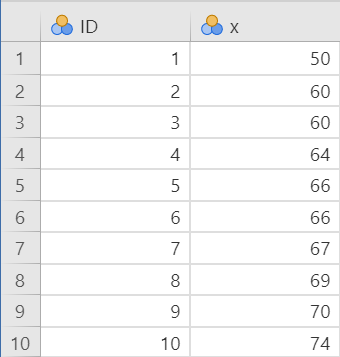
\includegraphics[width=0.8\linewidth]{images/07.1-one_sample_t-test/data} 

}

\caption{One-sample t-test data in jamovi}\label{fig:unnamed-chunk-1}
\end{figure}

\hypertarget{describe-the-data}{%
\subsubsection{Describe the data}\label{describe-the-data}}

Once we confirm our data is setup correctly in jamovi, we should look at our data using descriptive statistics and graphs. First, our descriptive statistics are shown below. Our overall data consists of 20 cases and the students in our dataset have a mean grade of 72.30 (\emph{SD} = 9.52). The minimum and maximum values look accurate; theoretically, student grades should range from 0-100. Lastly, the distribution of data looks possibly not normally distributed. Although we have a pretty small sample size, we can proceed with our analyses. First, though, we need to check our assumptions.

\begin{figure}

{\centering 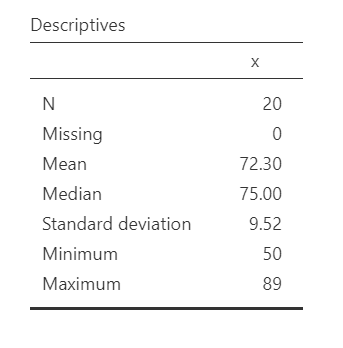
\includegraphics[width=0.8\linewidth]{images/07.1-one_sample_t-test/descriptives} 

}

\caption{Descriptive statistics}\label{fig:unnamed-chunk-2}
\end{figure}

\begin{figure}

{\centering 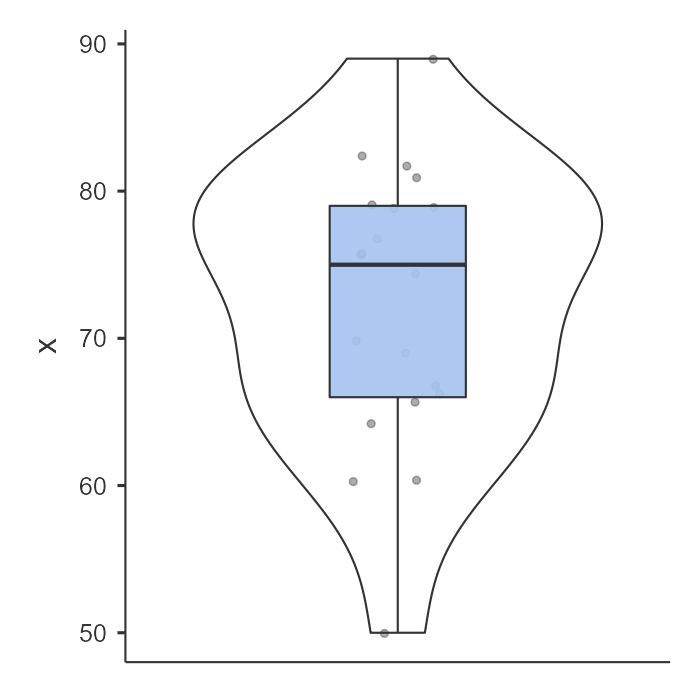
\includegraphics[width=0.8\linewidth]{images/07.1-one_sample_t-test/plot} 

}

\caption{Plot of the data}\label{fig:unnamed-chunk-3}
\end{figure}

\hypertarget{check-assumptions}{%
\subsection{Check assumptions}\label{check-assumptions}}

\hypertarget{assumptions}{%
\subsubsection{Assumptions}\label{assumptions}}

As a parametric test, the independent t-test has the same assumptions as other parametric tests:

\begin{enumerate}
\def\labelenumi{\arabic{enumi}.}
\item
  The dependent variable is \textbf{normally distributed}
\item
  The dependent variable is \textbf{interval or ratio} (i.e., continuous)
\item
  Scores are \textbf{independent} between groups
\end{enumerate}

We cannot test the second and third assumptions; rather, those are based on knowing your data.

However, we can and should test for the first assumption. Fortunately, the independent samples t-test in jamovi has two check boxes under ``Assumption Checks'' that lets us test for normality.

\hypertarget{checking-assumptions}{%
\subsubsection{Checking assumptions}\label{checking-assumptions}}

One thing to keep in mind in all statistical software is that we often check assumptions simultaneously to performing the statistical test. However, we should always check assumptions first before looking at and interpreting our results. Therefore, whereas the instructions for performing the test are below, we discuss checking assumptions here first to help ingrain the importance of always checking assumptions for interpreting results.

\hypertarget{testing-normality}{%
\paragraph{Testing normality}\label{testing-normality}}

jamovi easily allows us to check for normality using the Shapiro-Wilk test and the Q-Q plot. The Shapiro-Wilk test was not statistically significant (W = .96, \emph{p} = .586); therefore, this indicates the data is normally distributed. Furthermore, the lines are fairly close to the diagonal line in the Q-Q plot. We can conclude that we satisfy the assumption of normality.

\begin{figure}

{\centering 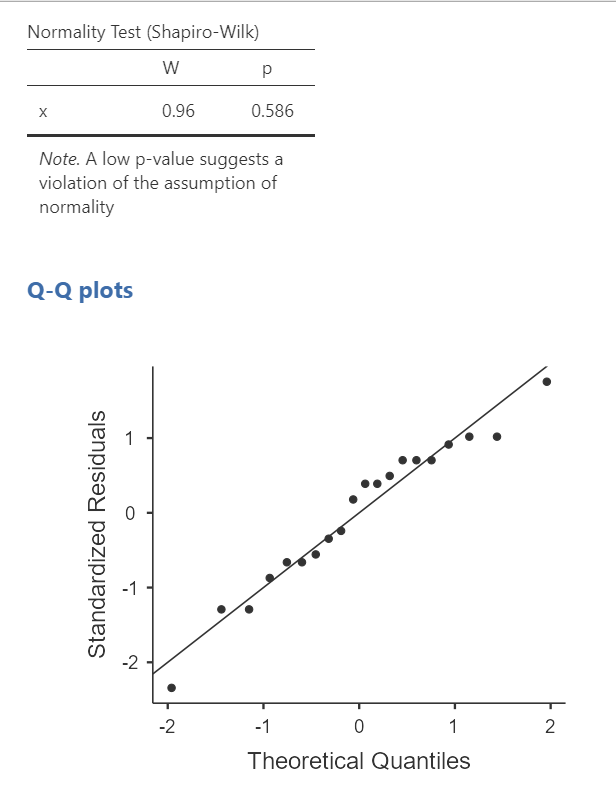
\includegraphics[width=1\linewidth]{images/07.1-one_sample_t-test/normality} 

}

\caption{Testing normality in jamovi}\label{fig:unnamed-chunk-4}
\end{figure}

Remember that we can also test for normality by \textbf{looking at our data} (e.g., a histogram or density plot, which you can see above) and by examining \textbf{skew and kurtosis}. However, you will need to view them using Exploration --\textgreater{} Descriptives, not in the t-tests menu. Here is our skew and kurtosis:

\begin{itemize}
\item
  \textbf{Skew}: \(-.53/.51 = -1.04\)
\item
  \textbf{Kurtosis}: \(.07/.99 = .07\)
\end{itemize}

Remember that we divide the value by its standard error to determine the z-score. If the absolute value of it is below 1.96 then we assume it is normally distributed. Both skew and kurtosis meet the assumption of normality. In addition, so did all our other pieces of evidence of normality: Shapiro-Wilk's, visual examination of the distribution, and the Q-Q plot. Therefore we can assume we met the assumption of normality.

\hypertarget{perform-the-test}{%
\subsection{Perform the test}\label{perform-the-test}}

Now that we've satisfied the assumptions, we can perform the one sample t-test. Here are the steps for doing so in jamovi:

\begin{enumerate}
\def\labelenumi{\arabic{enumi}.}
\item
  Go to the Analyses tab, click the T-Tests button, and choose ``One Sample T-Test''.
\item
  Move your dependent variable \texttt{x} to the Dependent Variables box.
\item
  Under Tests, select \texttt{Student\textquotesingle{}s}. We'll learn about Wilcoxon rank when we discuss violated assumptions.
\item
  Under Hypothesis, input the population mean. In our case, it is \texttt{67.5} (this is the mean given to us by Dr.~Zeppo). Also, select the hypothesis that matches your hypothesi. In our case, select \texttt{\textgreater{}\ Test\ value} because we believe psychology students have a higher mean than the test value (population mean).
\item
  Under Additional Statistics, select \texttt{Mean\ difference}, \texttt{Effect\ size}, \texttt{Descriptives}, and (optionally) \texttt{Descriptives\ plots}.
\item
  Under Assumption Checks, select both options: \texttt{Normality\ test} and \texttt{Q-Q\ plot}.
\end{enumerate}

When you are done, your setup should look like this:

\begin{figure}

{\centering 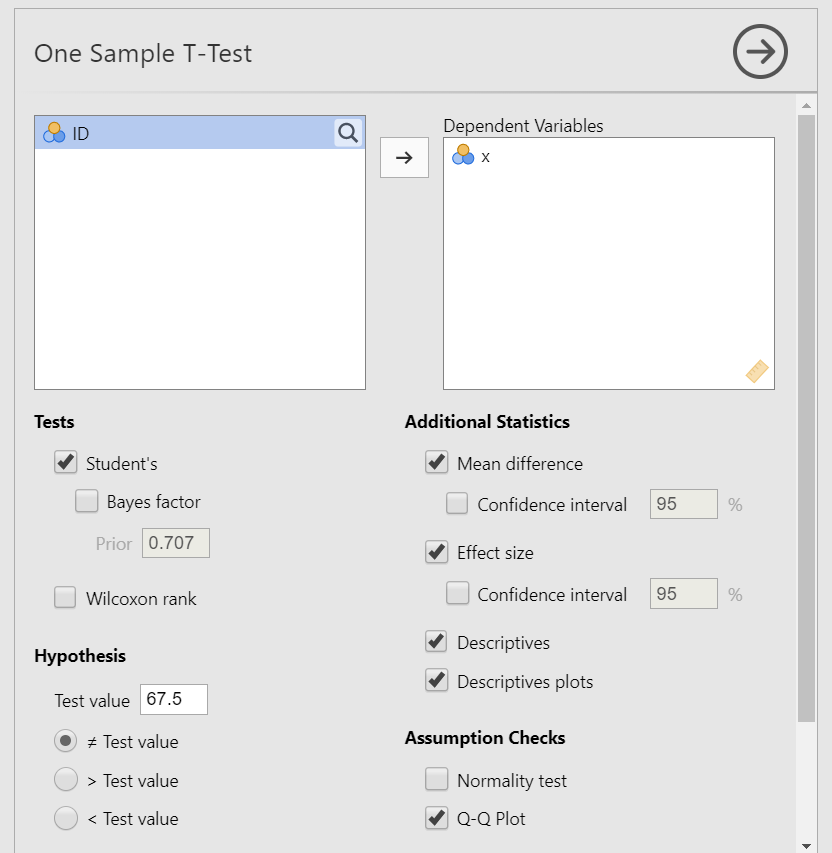
\includegraphics[width=0.8\linewidth]{images/07.1-one_sample_t-test/setup} 

}

\caption{One sample t-test setup in jamovi}\label{fig:unnamed-chunk-5}
\end{figure}

\hypertarget{interpret-results}{%
\subsection{Interpret results}\label{interpret-results}}

Once we are satisfied we have satisfied the assumptions for the independent t-test, we can interpret our results.

\begin{figure}

{\centering 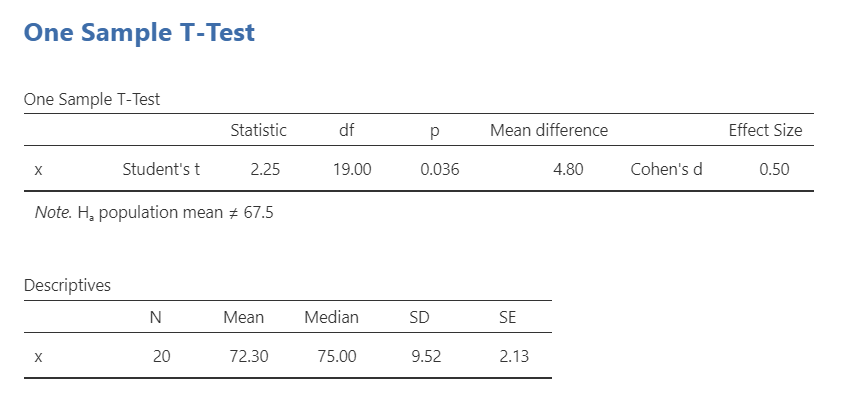
\includegraphics[width=1\linewidth]{images/07.1-one_sample_t-test/results} 

}

\caption{One sample t-test results in jamovi}\label{fig:unnamed-chunk-6}
\end{figure}

Our p-value is less than .05, so our results are statistically significant. Like most of the statistics we'll come across, the larger the t-statistic (or F-statistic, or chi-square statistic\ldots), the smaller the p-value will be. Therefore, we reject our null hypothesis that the population mean is less than or equal to the sample mean of psychology students.

\hypertarget{write-up-the-results-in-apa-style}{%
\subsubsection{Write up the results in APA style}\label{write-up-the-results-in-apa-style}}

When writing up the results of a statistical test, we should always include the following information:

\begin{enumerate}
\def\labelenumi{\arabic{enumi}.}
\tightlist
\item
  Description of your research question.
\item
  Description of your data. If you fail to meet assumptions, you should specify that and describe what test you chose to perform as a result.
\item
  The results of the inferential test, including what test was performed, the test value and degrees of freedom, p-value, and effect size.
\item
  Interpretation of the results, including any other information as needed.
\end{enumerate}

We can write up our results in APA something like this:

\begin{quote}
Dr.~Zeppo's psychology colleague hypothesized that his psychology students have a higher grade than the population of his students. Psychology students (\emph{M} = 72.30, \emph{SD} = 9.52, \emph{n} = 20) had significantly higher grades than the population of Dr.~Zeppo's students (\emph{M} = 67.50), \emph{t} (19) = 2.25, \emph{p} = .046, \emph{d} = .50.
\end{quote}

Let's analyze that against the 4 things we need to report:

\begin{quote}
\textbf{\#1} Dr.~Zeppo's psychology colleague hypothesized that his psychology students have a higher grade than the population of his students. \textbf{\#4} Psychology students \textbf{\#2} (\emph{M} = 72.30, \emph{SD} = 9.52, \emph{n} = 20) had significantly higher grades than the population of Dr.~Zeppo's students (\emph{M} = 67.50), \textbf{\#3} \emph{t} (19) = 2.25, \emph{p} = .046, \emph{d} = .50.
\end{quote}

Note that this is not the only way we can write up the results in APA format. The key is that we include all four pieces of information as specified above.

\hypertarget{visualize-the-results}{%
\subsubsection{Visualize the results}\label{visualize-the-results}}

By selecting \texttt{Descriptives\ plots} in the setup, you get the figure below. Personally, I don't think this is a very good plot. It's not very informative. It just provides the mean (circle), 95\% confidence interval (blue bars), and the median.

\begin{figure}

{\centering 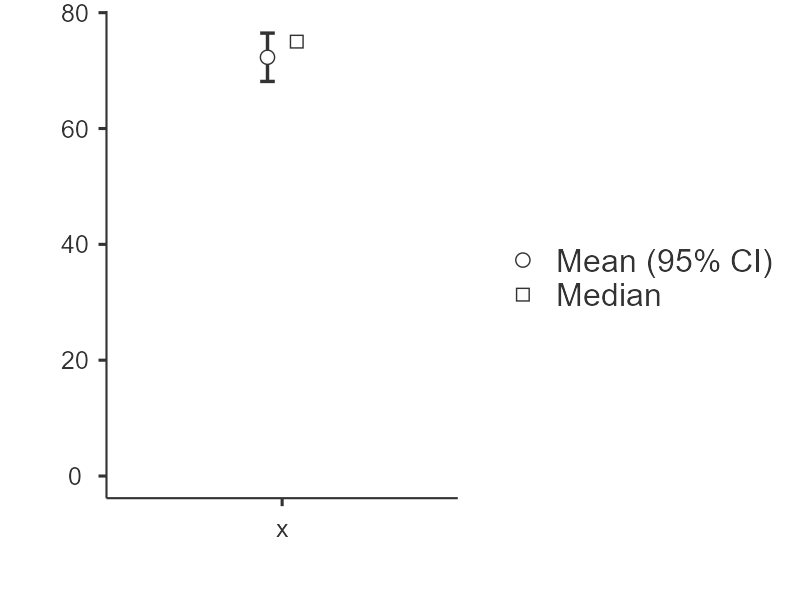
\includegraphics[width=1\linewidth]{images/07.1-one_sample_t-test/results-plot} 

}

\caption{One sample t-test descriptives plot}\label{fig:unnamed-chunk-7}
\end{figure}

Another default option in jamovi is via the Descriptives analysis. You can ask for the boxplot, violin plot, and data of your dependent variable split by your independent variable. This is a much better option. Not only does it show us our mean (black bars) and interquartile range (via the boxplot), but it also shows our distribution (violin plot) and data points (grey dots). This is much more informative. You can see this in the Look at your data section above.

\hypertarget{in-case-of-violated-assumptions}{%
\subsection{In case of violated assumptions}\label{in-case-of-violated-assumptions}}

If you fail to meet the assumption of normality, and no transformation fixes the data, then you can use the Wilcoxon W test.

The Wilcoxon W is not calculated based on the mean but rather the median. It has no assumptions about the distribution of data. Therefore, it is a non-parametric test. Here is what the output for the student's t-test and Wilcoxon W look like in jamovi:

\begin{figure}

{\centering 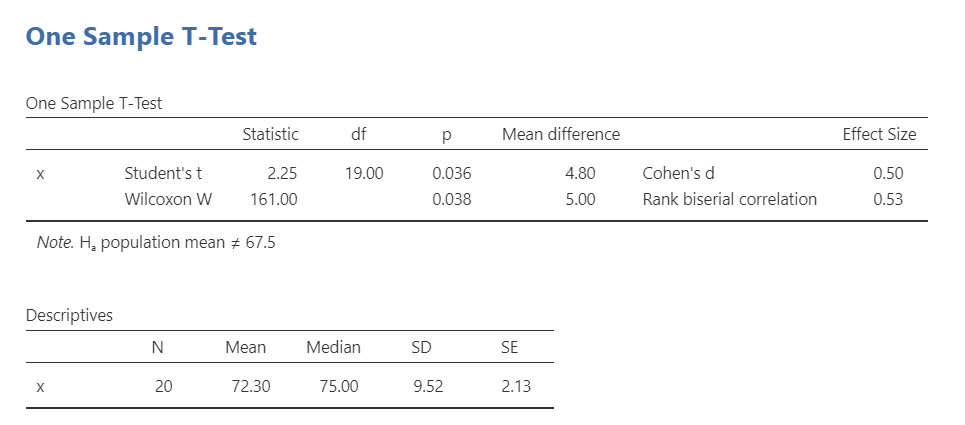
\includegraphics[width=1\linewidth]{images/07.1-one_sample_t-test/wilcoxon} 

}

\caption{All one sample t-test results in jamovi}\label{fig:unnamed-chunk-8}
\end{figure}

\hypertarget{wilcoxon-w-in-jamovi}{%
\paragraph{Wilcoxon W in jamovi}\label{wilcoxon-w-in-jamovi}}

To conduct this in jamovi, under Tests select \texttt{Wilcoxon\ W}. You will interpret the results similarly to the one sample t-test:

\begin{quote}
Dr.~Zeppo's psychology colleague hypothesized that his psychology students have a higher grade than the population of his students. Using a Wilcoxon W test, psychology students (\emph{Mdn} = 75.00, \emph{SD} = 9.52, \emph{n} = 20) had a higher grade than the population of Dr.~Zeppo's students (\emph{M} = 67.5), \emph{W} = 161, \emph{p} = .038, \(r_{bn}\) = .53.
\end{quote}

Note that we no longer report the mean but rather the median. That is because Wilcoxon W is based on the median, not the mean score.

\hypertarget{additional-information}{%
\subsection{Additional information}\label{additional-information}}

\hypertarget{positive-and-negative-t-values}{%
\subsubsection{Positive and negative t values}\label{positive-and-negative-t-values}}

Students often worry about positive or negative t-statistic values and are unsure how to interpret it. Positive or negative t-statistic values simply occur based on which group is listed first. Our t-statistic above is positive because we tested the difference between Anastasia and Bernadette: (Anastasia - Bernadette) = (74.53 - 69.06) = (5.48).

However, if we flipped it and tested the difference between Bernadette and Anastasia, our mean difference would be -5.48 and our t-statistic would be -2.12.

All that is to say, \emph{your positive or negative t-statistic is arbitrary}. So do not fret!

However, it is important the sign of your t-statistic matches what you report. For example, notice the difference:

\begin{quote}
\begin{enumerate}
\def\labelenumi{\arabic{enumi}.}
\tightlist
\item
  Anastasia's students had \textbf{higher} grades than Bernadette's, \emph{t} (31) = \textbf{2.12}, \emph{p} = .043, \emph{d} = \textbf{.74}.
\item
  Bernadette's students had \textbf{lower} grades than Anastasia's, \emph{t} (31) = \textbf{-2.12}, \emph{p} = .043, \emph{d} = \textbf{-.74}.
\end{enumerate}
\end{quote}

One last note: this positive or negative t-statistic is only relevant for the independent and dependent t-test. You will not get negative values for the F-statistic or chi-square tests!

\hypertarget{your-turn}{%
\subsection{Your turn!}\label{your-turn}}

Open the \texttt{Sample\_Dataset\_2014.xlsx} file that we will be using for all Your Turn exercises. You can find the dataset here: \href{https://github.com/danawanzer/stats-with-jamovi/blob/master/data/Sample_Dataset_2014.xlsx}{Sample\_Dataset\_2014.xlsx Download}

Perform one sample t-tests based on the following research questions. Think critically about whether you should be using a one-tailed or two-tailed hypothesis and check your assumptions so you know which test to use!

To get the most out of these exercises, try to first find out the answer on your own and then use the drop-down menus to check your answer.

\begin{enumerate}
\def\labelenumi{\arabic{enumi}.}
\item
  \textbf{Do the students in our dataset have a higher Writing score than passing (\emph{M} = 70)?}

  \begin{itemize}
  \item
    Should you use a one-tailed or two-tailed hypothesis? one-tailed two-tailed
  \item
    Which statistic should you use based on your assumptions? Student's one sample t-test Wilcoxon rank one sample t-test
  \item
    Do the students in our dataset have a higher Writing score than passing (\emph{M} = 70)? yes no
  \end{itemize}
\item
  \textbf{Do the students in our dataset have the same national average height of college students (\emph{M} = 68 inches)?}

  \begin{itemize}
  \item
    Should you use a one-tailed or two-tailed hypothesis? one-tailed two-tailed
  \item
    Which statistic should you use based on your assumptions? Student's one sample t-test Wilcoxon rank one sample t-test
  \item
    Do the students in our dataset have the same national average height of college students)? yes no
  \end{itemize}
\end{enumerate}

\hypertarget{independent-t-test}{%
\section{Independent t-test}\label{independent-t-test}}

\hypertarget{overview-1}{%
\subsection{Overview}\label{overview-1}}

The independent t-test is used to test the difference in our dependent variable between two different groups of observations. Our grouping variable is our independent variable. In other words, we use the independent t-test when we have a research question with a \textbf{continuous dependent variable} and a \textbf{categorical independent variable with two categories in which \underline{different} participants are in each category}.

The independent t-test is also called the independent samples t-test and the Student's t-test.

There are three different types of alternative hypotheses we could have for the independent t-test:

\begin{enumerate}
\def\labelenumi{\arabic{enumi}.}
\item
  \textbf{Two-tailed}

  \begin{itemize}
  \tightlist
  \item
    \(H_1\): Group 1 has a different mean than Group 2.
  \item
    \(H_0\): There is no difference in means between the two groups.
  \end{itemize}
\item
  \textbf{One-tailed}

  \begin{itemize}
  \tightlist
  \item
    \(H_1\): Group 1 has a greater mean than Group 2.
  \item
    \(H_0\): The mean for Group 1 is less than or equal to the mean for Group 2.
  \end{itemize}
\item
  \textbf{One-tailed}

  \begin{itemize}
  \tightlist
  \item
    \(H_1\): Group 1 has a smaller mean than Group 2.
  \item
    \(H_0\): The mean for Group 1 is greater than or equal to the mean for Group 2.
  \end{itemize}
\end{enumerate}

\hypertarget{look-at-the-data-1}{%
\subsection{Look at the data}\label{look-at-the-data-1}}

For this chapter, we're going to work with data from lsj-data. Open data from your Data Library in ``lsj-data''. Select and open ``Harpo''.This dataset is hypothetical data of 33 students taking Dr.~Harpo's statistics lectures. We have two tutors for the class, Anastasia (\emph{n} = 15) and Bernadette (\emph{n} = 18). Our research question is ``Which tutor results in better student grades?'' We don't have a hypothesis that one does better than the other. Therefore our hypotheses can be written up as such:

\begin{itemize}
\tightlist
\item
  \(H_1\): There is a difference in student grades between Anastasia's and Bernadette's classes.
\item
  \(H_0\): There is no difference in student grades between Anastasia's and Bernadette's classes.
\end{itemize}

\hypertarget{data-set-up-1}{%
\subsubsection{Data set-up}\label{data-set-up-1}}

To conduct the independent t-test, we first need to ensure our data is set-up properly in our dataset. This requires having two columns: one with our continuous dependent variable and one indicating which group the participant is in. Each row is a unique participant or unit of analysis.

Below is the first ten rows of our data from the Harpo dataset.

\begin{figure}

{\centering 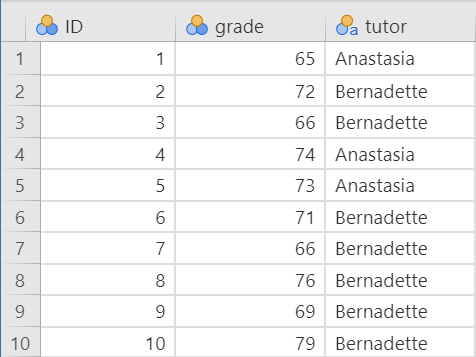
\includegraphics[width=0.8\linewidth]{images/02-independent_t-test/independent_t-test_data} 

}

\caption{Independent t-test data in jamovi}\label{fig:unnamed-chunk-1}
\end{figure}

In the data above, what is your \textbf{independent variable}? ID grade tutor

In the data above, what is your \textbf{dependent variable}? ID grade tutor

\hypertarget{describe-the-data-1}{%
\subsubsection{Describe the data}\label{describe-the-data-1}}

Once we confirm our data is setup correctly in jamovi, we should look at our data using descriptive statistics and graphs. First, our descriptive statistics are shown below. Our overall data consists of 33 cases and the students in our dataset have a mean grade of 71.55 (SD = 7.80). The minimum and maximum values look accurate; theoretically, student grades should range from 0-100. Lastly, the distribution of data looks nice and normally distributed. Although we have a pretty small sample size, especially within each group, we can proceed with our analyses. First, though, we need to check our assumptions.

\begin{figure}

{\centering 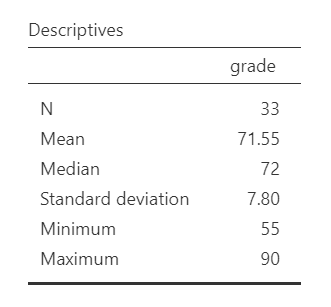
\includegraphics[width=0.8\linewidth]{images/02-independent_t-test/independent_t-test_descriptives_all} 

}

\caption{Descriptive statistics}\label{fig:unnamed-chunk-2}
\end{figure}

\begin{figure}

{\centering 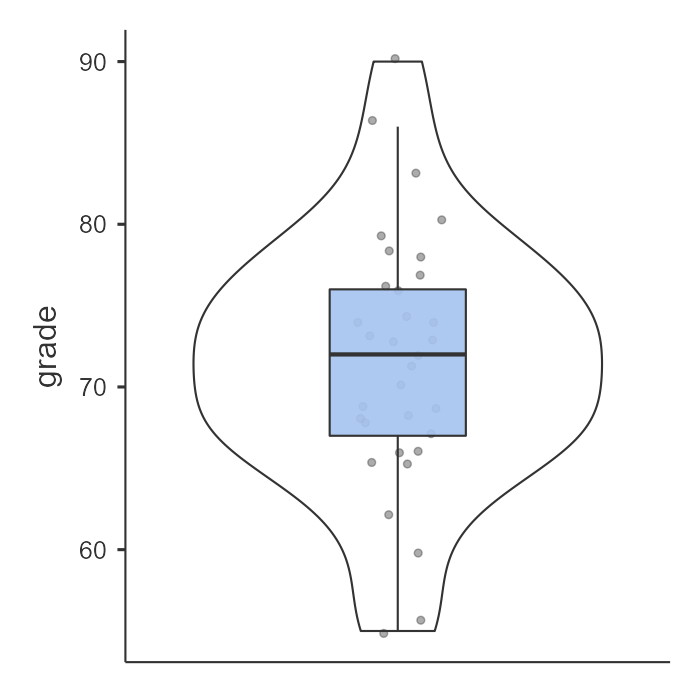
\includegraphics[width=0.8\linewidth]{images/02-independent_t-test/independent_t-test_plot_all} 

}

\caption{Plot of the data}\label{fig:unnamed-chunk-3}
\end{figure}

\hypertarget{check-assumptions-1}{%
\subsection{Check assumptions}\label{check-assumptions-1}}

\hypertarget{assumptions-1}{%
\subsubsection{Assumptions}\label{assumptions-1}}

As a parametric test, the independent t-test has the same assumptions as other parametric tests:

\begin{enumerate}
\def\labelenumi{\arabic{enumi}.}
\item
  The dependent variable is \textbf{normally distributed}
\item
  Variances in the two groups are roughly equal (i.e., \textbf{homogeneity of variances})
\item
  The dependent variable is \textbf{interval or ratio} (i.e., continuous)
\item
  Scores are \textbf{independent} between groups
\end{enumerate}

We cannot test the third and fourth assumptions; rather, those are based on knowing your data.

However, we can and should test for the first two assumptions. Fortunately, the independent samples t-test in jamovi has two check boxes under ``Assumption Checks'' that lets us test for both assumptions.

\hypertarget{checking-assumptions-1}{%
\subsubsection{Checking assumptions}\label{checking-assumptions-1}}

One thing to keep in mind in all statistical software is that we often check assumptions simultaneously to performing the statistical test. However, we should always check assumptions first before looking at and interpreting our results. Therefore, whereas the instructions for performing the test are below, we discuss checking assumptions here first to help ingrain the importance of always checking assumptions for interpreting results.

\hypertarget{testing-normality-1}{%
\paragraph{Testing normality}\label{testing-normality-1}}

jamovi easily allows us to check for normality using the Shapiro-Wilk test and the Q-Q plot. The Shapiro-Wilk test was not statistically significant (W = .98, \emph{p} = .827); therefore, this indicates the data is normally distributed. Furthermore, the lines are fairly close to the diagonal line in the Q-Q plot. We can conclude that we satisfy the assumption of normality.

\begin{figure}

{\centering 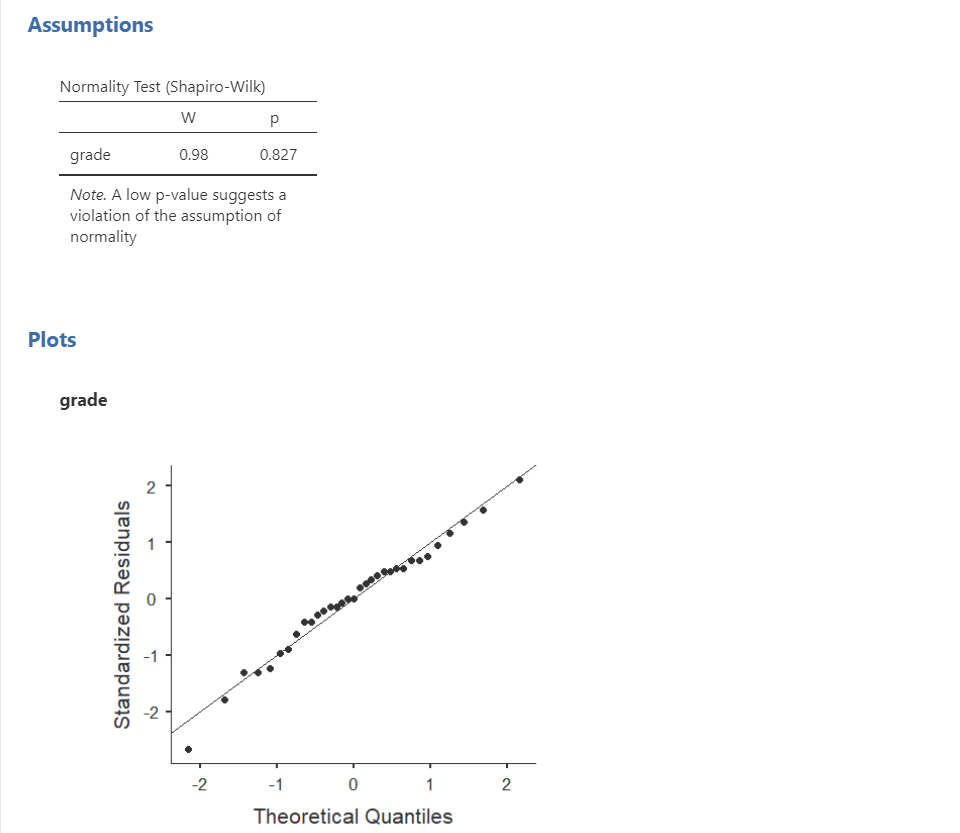
\includegraphics[width=1\linewidth]{images/02-independent_t-test/independent_t-test_normality} 

}

\caption{Testing normality in jamovi}\label{fig:unnamed-chunk-4}
\end{figure}

Remember that we can also test for normality by \textbf{looking at our data} (e.g., a histogram or density plot, which you can see above) and by examining \textbf{skew and kurtosis}. However, you will need to view them using Exploration --\textgreater{} Descriptives, not in the t-tests menu. Here is our skew and kurtosis:

\begin{itemize}
\item
  \textbf{Skew}: \(.06/.41 = .15\)
\item
  \textbf{Kurtosis}: \(.33/.80 = .41\)
\end{itemize}

Remember that we divide the value by its standard error to determine the z-score. If the absolute value of it is below 1.96 then we assume it is normally distributed. Both skew and kurtosis meet the assumption of normality. In addition, so did all our other pieces of evidence of normality: Shapiro-Wilk's, visual examination of the distribution, and the Q-Q plot. Therefore we can assume we met the assumption of normality.

\begin{figure}

{\centering 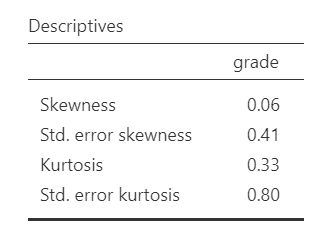
\includegraphics[width=0.8\linewidth]{images/02-independent_t-test/independent_t-test_skewkurtosis} 

}

\caption{Plot of the data}\label{fig:unnamed-chunk-5}
\end{figure}

\hypertarget{testing-homogeneity-of-variance}{%
\paragraph{Testing homogeneity of variance}\label{testing-homogeneity-of-variance}}

We test for homogeneity of variance using the Levene's test. The Levene's test was not statistically significant (\emph{F} {[}1, 31{]} = 2.49, \emph{p} = .125); therefore, this indicates our data satisfies the assumption of homogeneity of variance. However, I would add a caveat that we have a small sample of data (\emph{n} = 15 for Anastasia and \emph{n} = 18 for Bernadette) and the standard deviations are quite different from one another (SD = 9.00 vs 5.77, respectively). We should have tried to collect more data.

\begin{figure}

{\centering 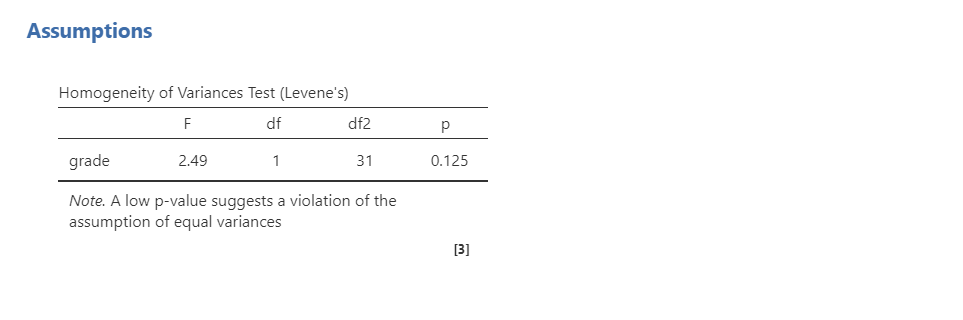
\includegraphics[width=1\linewidth]{images/02-independent_t-test/independent_t-test_homogeneity} 

}

\caption{Testing homogeneity of variance in jamovi}\label{fig:unnamed-chunk-6}
\end{figure}

\hypertarget{perform-the-test-1}{%
\subsection{Perform the test}\label{perform-the-test-1}}

Now that we've satisfied the assumptions, we can perform the independent t-test. Here are the steps for doing so in jamovi:

\begin{enumerate}
\def\labelenumi{\arabic{enumi}.}
\item
  Go to the Analyses tab, click the T-Tests button, and choose ``Independent Samples T-Test''.
\item
  Move your dependent variable \texttt{grade} to the Dependent Variables box and your independent variable \texttt{tutor} to the Grouping Variable box.
\item
  Under Tests, select \texttt{Student\textquotesingle{}s}. We'll learn about Welch's and Mann-Whitney U under the violated assumptions section.
\item
  Under Hypothesis, select the hypothesis that matches your research question. In our case, select \texttt{Group\ 1\ ≠\ Group\ 2} because we have a two-sided hypothesis.
\item
  Under Additional Statistics, select \texttt{Mean\ difference}, \texttt{Effect\ size}, \texttt{Descriptives}, and (optionally) \texttt{Descriptives\ plots}.
\item
  Under Assumption Checks, select all three options: \texttt{Homogeneity\ test}, \texttt{Normality\ test}, and \texttt{Q-Q\ plot}.
\end{enumerate}

When you are done, your setup should look like this

\begin{figure}

{\centering 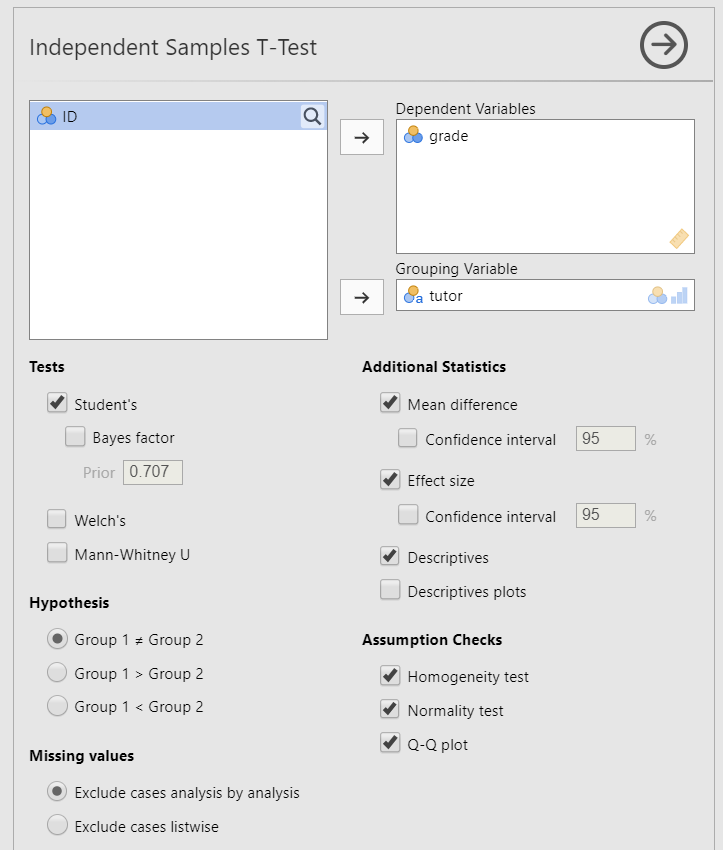
\includegraphics[width=0.8\linewidth]{images/02-independent_t-test/independent_t-test_setup} 

}

\caption{Independent t-test setup in jamovi}\label{fig:unnamed-chunk-7}
\end{figure}

\hypertarget{interpret-results-1}{%
\subsection{Interpret results}\label{interpret-results-1}}

Once we are satisfied we have satisfied the assumptions for the independent t-test, we can interpret our results.

\begin{figure}

{\centering 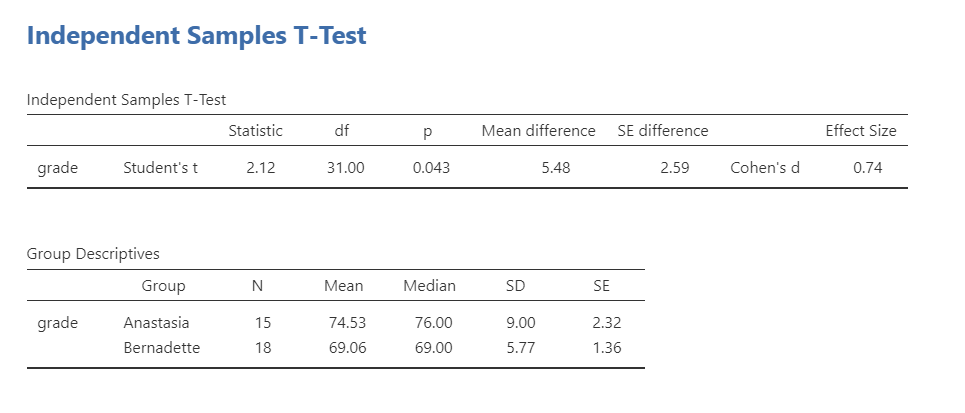
\includegraphics[width=1\linewidth]{images/02-independent_t-test/independent_t-test_ind-results} 

}

\caption{Independent t-test results in jamovi}\label{fig:unnamed-chunk-8}
\end{figure}

Our p-value is less than .05, so our results are statistically significant. Like most of the statistics we'll come across, the larger the t-statistic (or F-statistic, or chi-square statistic\ldots), the smaller the p-value will be. Therefore, we reject our null hypothesis that there is no difference between the two groups.

\hypertarget{write-up-the-results-in-apa-style-1}{%
\subsubsection{Write up the results in APA style}\label{write-up-the-results-in-apa-style-1}}

When writing up the results of a statistical test, we should always include the following information:

\begin{enumerate}
\def\labelenumi{\arabic{enumi}.}
\tightlist
\item
  Description of your research question.
\item
  Description of your data. If you fail to meet assumptions, you should specify that and describe what test you chose to perform as a result.
\item
  The results of the inferential test, including what test was performed, the test value and degrees of freedom, p-value, and effect size.
\item
  Interpretation of the results, including any other information as needed.
\end{enumerate}

We can write up our results in APA something like this:

\begin{quote}
The research question was whether there was a difference in student grades between Anastasia's and Bernadette's classes. Anastasia's students (\emph{M} = 74.53, \emph{SD} = 9.00, \emph{n} = 15) had significantly higher grades than Bernadette's students (\emph{M} = 69.06, \emph{SD} = 5.77, \emph{n}~= 18), \emph{t} (31) = 2.12, \emph{p} = .043, \emph{d} = .74.
\end{quote}

Let's analyze that against the 4 things we need to report:

\begin{quote}
\textbf{\#1:} The research question was whether there was a difference in student grades between Anastasia's and Bernadette's classes. \textbf{\#4} Anastasia's students \textbf{\#2} (\emph{M} = 74.53, \emph{SD} = 9.00, \emph{n} = 15) had significantly higher grades than Bernadette's students \textbf{\#2} (\emph{M} = 69.06, \emph{SD} = 5.77, \emph{n}~= 18), \textbf{\#3} \emph{t} (31) = 2.12, \emph{p} = .043, \emph{d} = .74.
\end{quote}

Sometimes, people like to put the statistics inside a parentheses. In that case, you need to change the parentheses around the degrees of freedom as brackets. Here's another example write-up of the results in APA style:

\begin{quote}
\textbf{\#1} I tested the difference in grades between Anastasia's students \textbf{\#2} (\emph{M} = 74.53, \emph{SD} = 9.00, \emph{n} = 15) and Bernadette's students (\emph{M} = 69.06, \emph{SD} = 5.77, \emph{n}~= 18). \textbf{\#3} An independent samples t-test showed that the 5.48 mean difference between the tutor's student was statistically significant (\emph{t} {[}31{]} = 2.12, \emph{p} = .043, \emph{d} = .74). \textbf{\#4} Therefore, we reject the null hypothesis that there is no difference in grades between the two classes.
\end{quote}

Note that these are not the only way we can write up the results in APA format. The key is that we include all four pieces of information as specified above.

\hypertarget{visualize-the-results-1}{%
\subsubsection{Visualize the results}\label{visualize-the-results-1}}

By selecting \texttt{Descriptives\ plots} in the setup, you get the figure below. Personally, I don't think this is a very good plot. It's not very informative. It just provides the mean (circle), 95\% confidence interval (blue bars), and the median.

\begin{figure}

{\centering 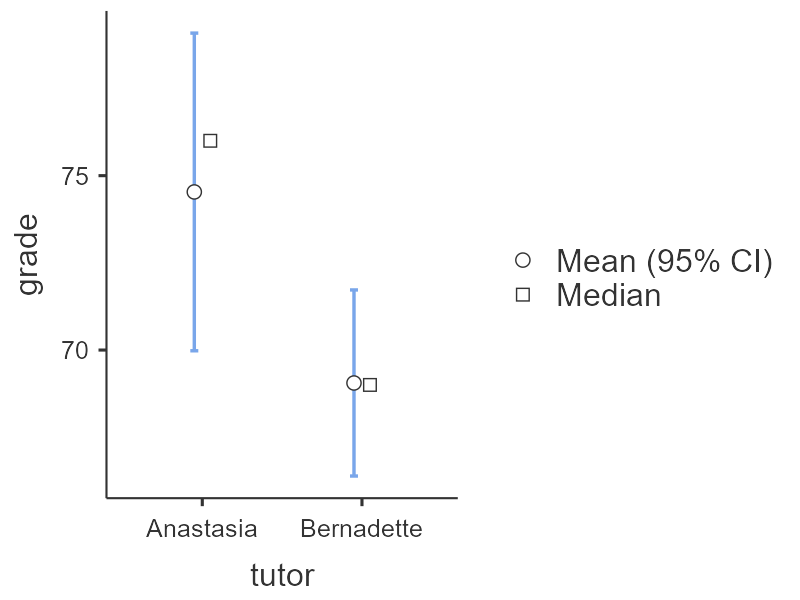
\includegraphics[width=1\linewidth]{images/02-independent_t-test/independent_t-test_plot2} 

}

\caption{Independent t-test descriptives plot}\label{fig:unnamed-chunk-9}
\end{figure}

Another default option in jamovi is via the Descriptives analysis. You can ask for the boxplot, violin plot, and data of your dependent variable split by your independent variable. This is a much better option. Not only does it show us our mean (black bars) and interquartile range (via the boxplot), but it also shows our distribution (violin plot) and data points (grey dots). This is much more informative.

\begin{figure}

{\centering 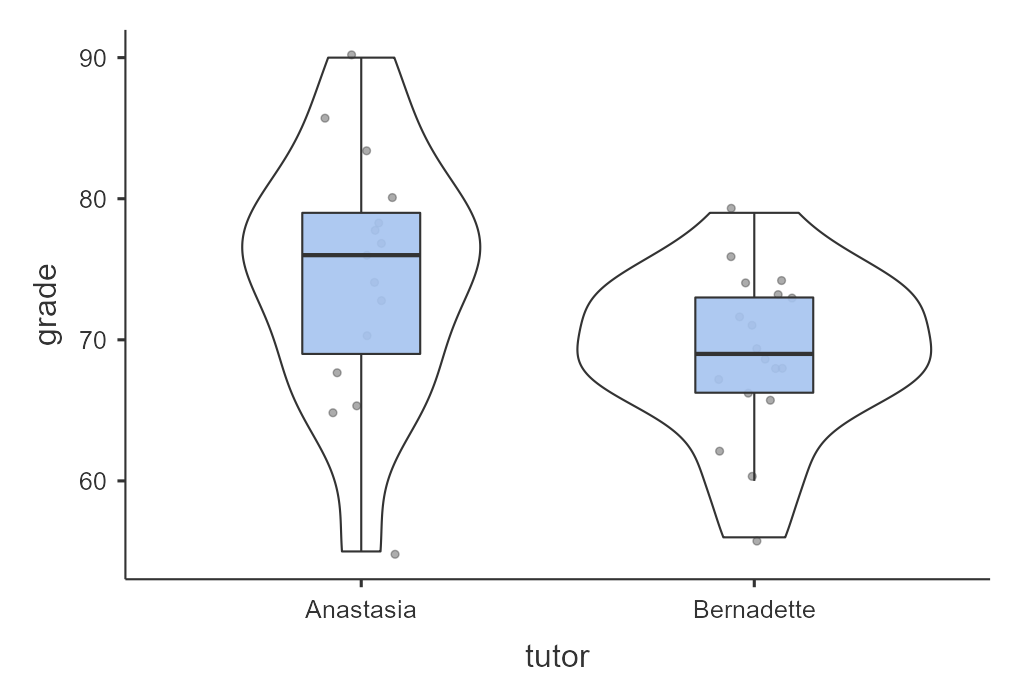
\includegraphics[width=1\linewidth]{images/02-independent_t-test/independent_t-test_plot} 

}

\caption{Independent t-test descriptives plot}\label{fig:unnamed-chunk-10}
\end{figure}

Oftentimes, people display results in a simple bar chart, often adding error bars (either 95\% CI or SE error bars). But this is also not a great chart because it lacks information about the underlying distribution of data. Therefore, for the independent t-test I recommend the visualization shown above.

\hypertarget{in-case-of-violated-assumptions-1}{%
\subsection{In case of violated assumptions}\label{in-case-of-violated-assumptions-1}}

If you fail to meet one or both of the assumptions of normality (and no transformations fixed your data) and homogeneity of variances, jamovi has the alternative statistics easily built in. Here's what statistic you should choose based on satisfying assumptions:

\begin{longtable}[]{@{}lll@{}}
\caption{Independent t-test to perform based on assumptions}\tabularnewline
\toprule
& \textbf{Normality: satisfied} & \textbf{Normality: not satisfied}\tabularnewline
\midrule
\endfirsthead
\toprule
& \textbf{Normality: satisfied} & \textbf{Normality: not satisfied}\tabularnewline
\midrule
\endhead
\textbf{Homogeneity of Variance: satisfied} & Student's t-test & Mann-Whitney U\tabularnewline
\textbf{Homogeneity of Variance: not satisfied} & Welch's t-test & Mann-Whitney U\tabularnewline
\bottomrule
\end{longtable}

The Welch's t-test has three main differences from the independent samples t-test: (a) the standard error (SE) is not a pooled estimate, (b) the degrees of freedom are calculated very different (not \emph{N} - 2), and (c) it does not have an assumption of homogeneity of variance. Note that Welch's t-test is \emph{not} a non-parametric test because it still has the assumption of a normal distribution.

The Mann-Whitney U is not calculated based on the mean but rather the median and compares ranks of values across the two groups: it has no assumptions about the distribution of data or homogeneity of variances. Therefore, it is a non-parametric test. Here is what the output for all three tests look like:

\begin{figure}

{\centering 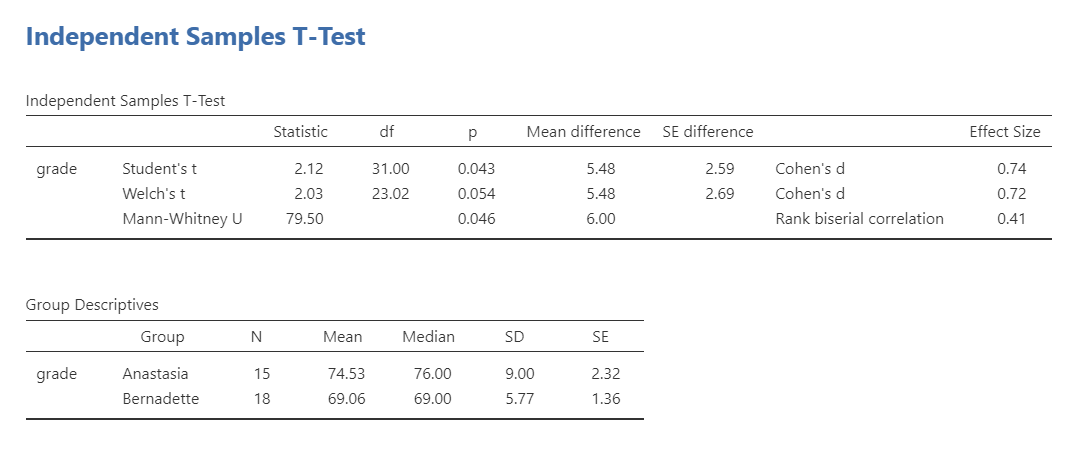
\includegraphics[width=1\linewidth]{images/02-independent_t-test/independent_t-test_full-results} 

}

\caption{All independent t-test results in jamovi}\label{fig:unnamed-chunk-11}
\end{figure}

\hypertarget{welchs-t-test}{%
\subsubsection{Welch's t-test}\label{welchs-t-test}}

To conduct this in jamovi, under Tests select \texttt{Welch\textquotesingle{}s}. You will interpret the results similarly to the independent t-test:

\begin{quote}
Using a Welch's t-test, there was not a statistically significant difference in grades between Anastasia's students (\emph{M} = 74.53, \emph{SD} = 9.00, \emph{n} = 15) and Bernadette's students (\emph{M} = 69.06, \emph{SD} = 5.77, \emph{n} = 18), \emph{t} (23.02) = 2.03, \emph{p} = .054, \emph{d} = .72.
\end{quote}

Why is it no longer statistically significant? Which result should you trust? In reality, the difference in \emph{p}-values is likely due to chance. However, the independent t-test and Welch's test have different strengths and weaknesses. If the two populations really do have equal variances, then the independent t-test is slightly more powerful (lower Type II error rate) than the Welch's test. However, if they \emph{don't} have the same variances, then the assumptions of the independent t-test are violated and you may not be able to trust the results; you may end up with a higher Type I error rate. So it's a trade-off.

Which should you use? I tend to prefer always using Welch's t-test because if the variances are equal, then there will be practically no difference between the independent and Welch's t-test. But if the variances are not equal, then Welch's t-test will outperform the independent t-test. For that reason, defaulting to the Welch's t-test makes most sense to me.

\hypertarget{mann-whitney-u-test}{%
\subsubsection{Mann-Whitney U test}\label{mann-whitney-u-test}}

If you do not satisfy the assumption of normality (regardless of whether you satisfy the assumption of homogeneity of variance), you should either try to transform your data to be normally distributed or you will need to use a non-parametric test. In this case, if you originally wanted to perform an independent t-test, the non-parametric equivalent test is the Mann-Whitney U test.

I will not go into specifics, but the idea behind the Mann-Whitney U test is that you take all the values (regardless of group) and rank them. You then sum the ranks across groups and calculate your U statistic and p-value. You interpret the p-value like you normally would, but there are differences in how we report the results because this statistic is based on the \emph{median} not the \emph{mean}.

\begin{quote}
Using the Mann-Whitney U test, there was a statistically significant difference in grades between Anastasia's students (\emph{Mdn} = 76, \emph{n} = 15) and Bernadette's students (\emph{Mdn} = 69, \emph{n}~= 18), \emph{U = 79.50}, \emph{p} = .054, \(r_{pb}\) = .41.
\end{quote}

\hypertarget{your-turn-1}{%
\subsection{Your turn!}\label{your-turn-1}}

Open the \texttt{Sample\_Dataset\_2014.xlsx} file that we will be using for all Your Turn exercises. You can find the dataset here: \href{https://github.com/danawanzer/stats-with-jamovi/blob/master/data/Sample_Dataset_2014.xlsx}{Sample\_Dataset\_2014.xlsx Download}

Perform independent t-tests based on the following research questions. Think critically about whether you should be using a one-tailed or two-tailed hypothesis and check your assumptions so you know which test to use!

To get the most out of these exercises, try to first find out the answer on your own and then use the drop-down menus to check your answer.

\begin{enumerate}
\def\labelenumi{\arabic{enumi}.}
\item
  \textbf{Does height differ by gender (Gender: male = 0, female = 1)?}

  \begin{itemize}
  \item
    Should you use a one-tailed or two-tailed hypothesis? one-tailed two-tailed
  \item
    Which statistic should you use based on your assumptions? independent t-test Welch's t-test Mann Whitney U
  \item
    Does height differ by gender? yes no
  \end{itemize}
\item
  \textbf{Do athletes (Athlete: athletes = 1, non-athlete = 0) have faster sprint times than non-athletes?}

  \begin{itemize}
  \item
    Should you use a one-tailed or two-tailed hypothesis? one-tailed two-tailed
  \item
    Which statistic should you use based on your assumptions? independent t-test Welch's t-test Mann Whitney U
  \item
    Do athletes have faster sprint times than non-athletes? yes no
  \end{itemize}
\item
  \textbf{Do students who live on campus (LiveOnCampus: on campus = 1, off campus = 0) have higher English scores than students who live off campus?}

  \begin{itemize}
  \item
    Should you use a one-tailed or two-tailed hypothesis? one-tailed two-tailed
  \item
    Which statistic should you use based on your assumptions? independent t-test Welch's t-test Mann Whitney U
  \item
    Does students who live on campus have higher English scores? yes no
  \end{itemize}
\item
  \textbf{Does athletic status relate to math scores?}

  \begin{itemize}
  \item
    Should you use a one-tailed or two-tailed hypothesis? one-tailed two-tailed
  \item
    Which statistic should you use based on your assumptions? independent t-test Welch's t-test Mann Whitney U
  \item
    Does athletic status relate to math scores? yes no
  \end{itemize}
\end{enumerate}

\hypertarget{dependent-t-test}{%
\section{Dependent t-test}\label{dependent-t-test}}

\hypertarget{overview-2}{%
\subsection{Overview}\label{overview-2}}

The dependent t-test is used to test the difference in our dependent variable between two categories in which participants are the \emph{same} across categories. Our category variable is our independent variable. In other words, we use the dependent t-test when we have a research question with a \textbf{continuous dependent variable} and a \textbf{categorical independent variable with two categories in which the \underline{same} participants are in each category}.

The dependent t-test is also called a dependent samples t-test or paired samples t-test.

There are three different types of alternative hypotheses we could have for the dependent t-test:

\begin{enumerate}
\def\labelenumi{\arabic{enumi}.}
\item
  \textbf{Two-tailed}

  \begin{itemize}
  \tightlist
  \item
    \(H_1\): There is a difference in means between the two time points or conditions.
  \item
    \(H_0\): There is no difference in means between the two time points or conditions.
  \end{itemize}
\item
  \textbf{One-tailed}

  \begin{itemize}
  \tightlist
  \item
    \(H_1\): The mean at time 1 or condition 1 is greater than the mean at time 2 or condition 2.
  \item
    \(H_0\): The mean at time 1 or condition 1 is less than or equal to the mean at time 2 or condition 2.
  \end{itemize}
\item
  \textbf{One-tailed}

  \begin{itemize}
  \tightlist
  \item
    \(H_1\): The mean at time 1 or condition 1 is smaller than the mean at time 2 or condition 2.
  \item
    \(H_0\): The mean at time 1 or condition 1 is greater than or equal to the mean at time 2 or condition 2.
  \end{itemize}
\end{enumerate}

\hypertarget{look-at-the-data-2}{%
\subsection{Look at the data}\label{look-at-the-data-2}}

For this chapter, we're going to work with data from lsj-data. Open data from your Data Library in ``lsj-data''. Select and open ``Chico''. This dataset is hypothetical data from Dr.~Chico's class in which students took two tests: one early in the semester and one later in the semester. Dr.~Chico thinks that the first test is a ``wake up call'' for students. When they realise how hard her class really is, they'll work harder for the second test and get a better mark. Is she right? First, let's determine our hypotheses:

What is Dr.~Chico's alternative hypothesis? test 1 scores are different from test 2 scores test 1 scores are greater than test 2 scores test 1 scores are less than test 2 scores

\hypertarget{data-set-up-2}{%
\subsubsection{Data set-up}\label{data-set-up-2}}

To conduct the dependent t-test, we first need to ensure our data is set-up properly in our dataset. This requires having two columns: one is our dependent variable score for the participant in one category and the other column is our dependent variable score for the participant in the other category. Each row is a unique participant or unit of analysis.

\begin{figure}

{\centering 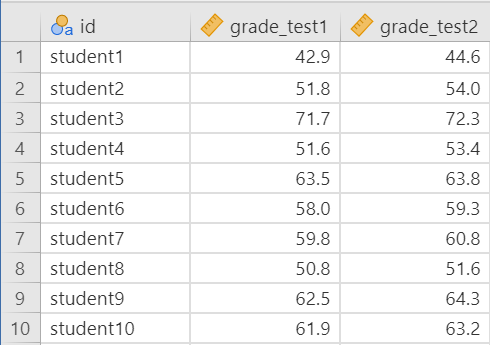
\includegraphics[width=0.8\linewidth]{images/03_dependent_t-test/dependent_data} 

}

\caption{Dependent t-test data in jamovi}\label{fig:unnamed-chunk-1}
\end{figure}

In the data above, what is your \textbf{independent variable}? id grade test score grade\_test1 grade\_test2

In the data above, what is your \textbf{dependent variable}? id grade test score grade\_test1 grade\_test2

\hypertarget{describe-the-data-2}{%
\subsubsection{Describe the data}\label{describe-the-data-2}}

Once we confirm our data is setup correctly in jamovi, we should look at our data using descriptive statistics and graphs. First, our descriptive statistics are shown below. Our overall data consists of 20 cases (students) and the average grade is 56.98 (\emph{SD} = 6.62) at the first test and 58.38 (\emph{SD} = 6.41) at the second test. We have no missing cases, and our minimum and maximum values look accurate; theoretically, student grades should range from 0-100. Lastly, the distribution of data looks fairly normally distributed, although I'm personally a little worried about our small sample size. Before we can proceed with our analyses, we'll need to check our assumptions.

\begin{figure}

{\centering 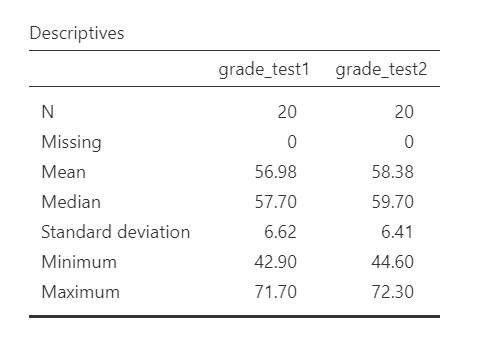
\includegraphics[width=0.8\linewidth]{images/03_dependent_t-test/dependent_descriptives} 

}

\caption{Descriptive statistics}\label{fig:unnamed-chunk-2}
\end{figure}

\begin{figure}

{\centering 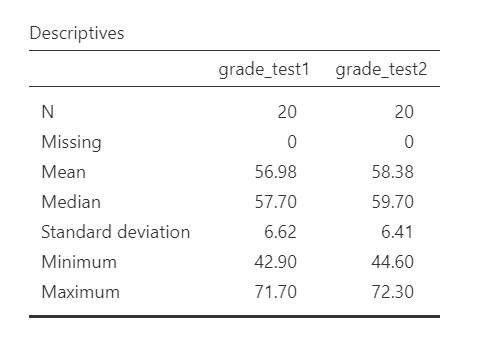
\includegraphics[width=0.8\linewidth]{images/03_dependent_t-test/dependent_descriptives} 

}

\caption{Descriptive statistics}\label{fig:unnamed-chunk-3}
\end{figure}

\begin{figure}

{\centering 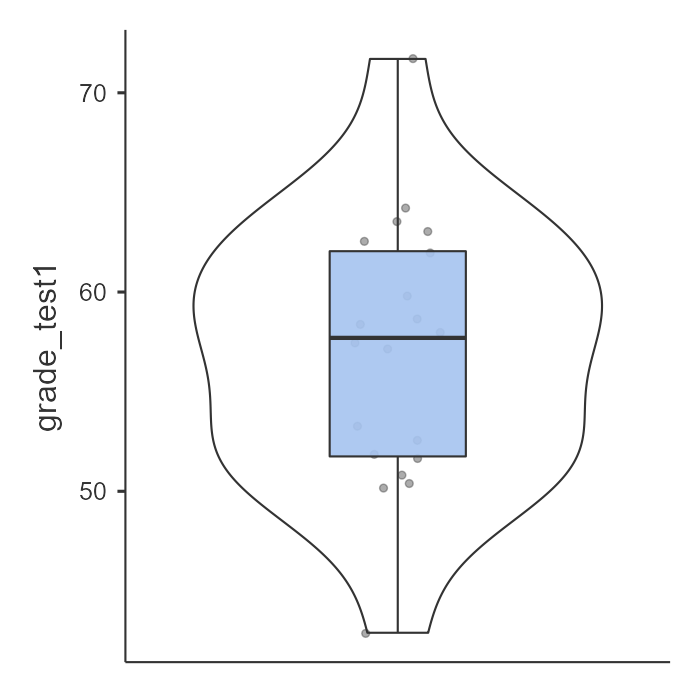
\includegraphics[width=0.49\linewidth]{images/03_dependent_t-test/dependent_plot1} 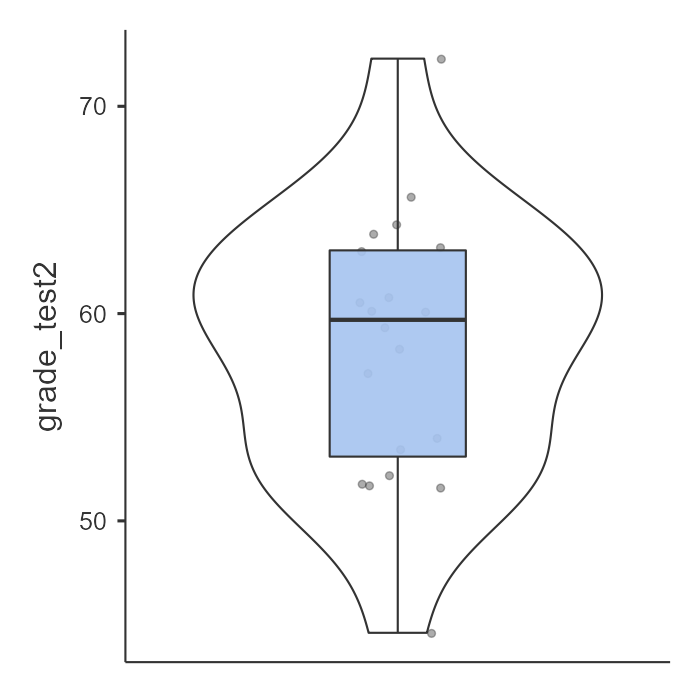
\includegraphics[width=0.49\linewidth]{images/03_dependent_t-test/dependent_plot2} 

}

\caption{Plots of the data}\label{fig:unnamed-chunk-4}
\end{figure}

\hypertarget{check-assumptions-2}{%
\subsection{Check assumptions}\label{check-assumptions-2}}

\hypertarget{assumptions-2}{%
\subsubsection{Assumptions}\label{assumptions-2}}

As a parametric test, the dependent t-test has the same assumptions as other parametric tests minus the homogeneity of variance assumption because we are dealing with the same people across categories

\begin{enumerate}
\def\labelenumi{\arabic{enumi}.}
\item
  The \emph{differences in scores} in the dependent variable are \textbf{normally distributed}
\item
  The dependent variable is \textbf{interval or ratio} (i.e., continuous)
\item
  Scores are \textbf{independent} \emph{across participants}
\end{enumerate}

We cannot \emph{test} the second and third assumptions; rather, those are based on knowing your data.

However, we can and should test for the first assumption. Fortunately, the dependent samples t-test in jamovi has two check boxes under ``Assumption Checks'' that lets us test normality.

\hypertarget{checking-assumptions-2}{%
\subsubsection{Checking assumptions}\label{checking-assumptions-2}}

One thing to keep in mind in all statistical software is that we often check assumptions simultaneously to performing the statistical test. However, we should always check assumptions first before looking at and interpreting our results. Therefore, whereas the instructions for performing the test are below, we discuss checking assumptions here first to help ingrain the importance of always checking assumptions for interpreting results.

\hypertarget{testing-normality-2}{%
\paragraph{Testing normality}\label{testing-normality-2}}

Notice how our dependent variable is really the difference in scores, and therefore that is what we are testing for normality. We test for normality using the Shapiro-Wilk test and the Q-Q plot. The Shapiro-Wilk test was not statistically significant (W = .97, \emph{p} = .678); therefore, this indicates the data is normally distributed. Furthermore, the lines are fairly close to the diagonal line in the Q-Q plot (although it's a bit hard to tell because our sample size is small). We can conclude that we satisfy the assumption of normality.

\begin{figure}

{\centering 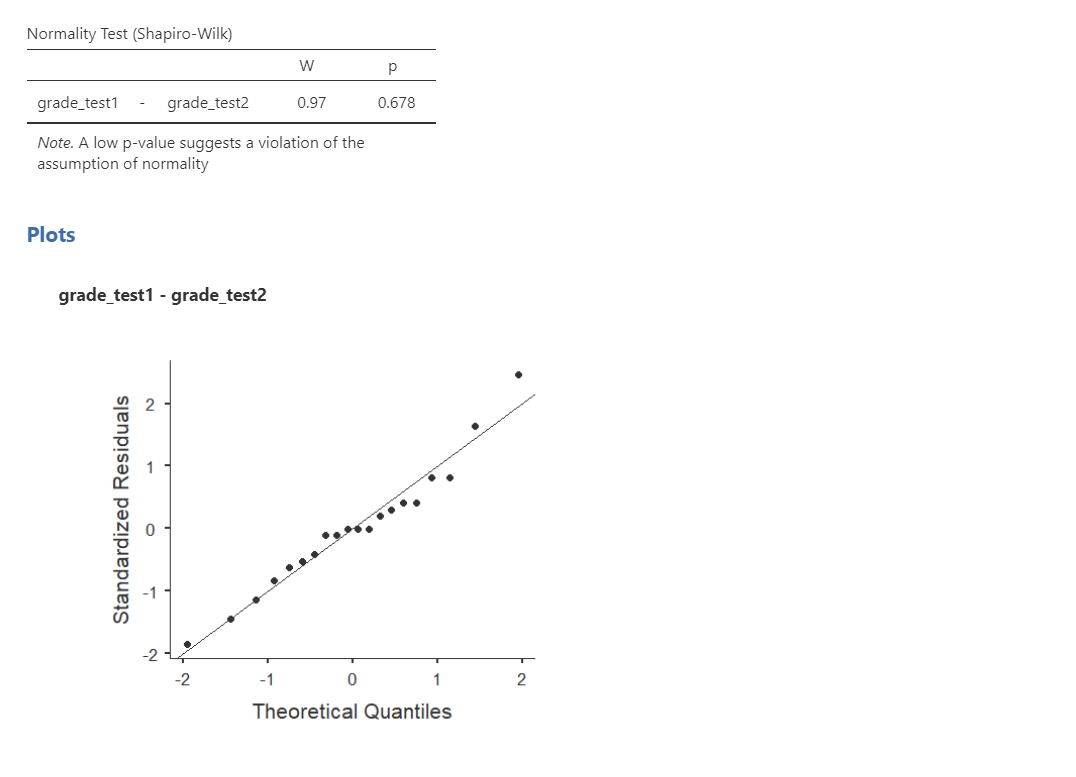
\includegraphics[width=1\linewidth]{images/03_dependent_t-test/dependent_normality} 

}

\caption{Testing normality in jamovi}\label{fig:unnamed-chunk-5}
\end{figure}

\hypertarget{perform-the-test-2}{%
\subsection{Perform the test}\label{perform-the-test-2}}

Now that we've satisfied the assumptions, we can perform the dependent t-test. Here are the steps for doing so in jamovi:

\begin{enumerate}
\def\labelenumi{\arabic{enumi}.}
\item
  Go to the Analyses tab, click the T-Tests button, and choose ``Paired Samples T-Test''.
\item
  Move both measurements of your dependent variable (\texttt{grade\_test1} and \texttt{grade\_test2}) to the Paired Variables box.
\item
  Under Tests, select \texttt{Student\textquotesingle{}s}. We'll learn more about the Wilcoxon rank option, which is an option if you fail to meet the assumption of normality.
\item
  Under Hypothesis, choose the correct hypothesis: Measure 1 is not equal to Measure 2 Measure 1 \textgreater{} Measure 2 Measure 1 \textless{} Measure 2
\item
  Under Additional Statistics, select \texttt{Mean\ difference}, \texttt{Effect\ size}, \texttt{Descriptives}, and (optionally) \texttt{Descriptives\ plots}.
\item
  Under Assumption Checks, select both options: \texttt{Normality\ test} and \texttt{Q-Q\ plot}. You'll check these assumptions first, which is discussed above.
\end{enumerate}

When you are done, your setup should look like this

\begin{figure}

{\centering 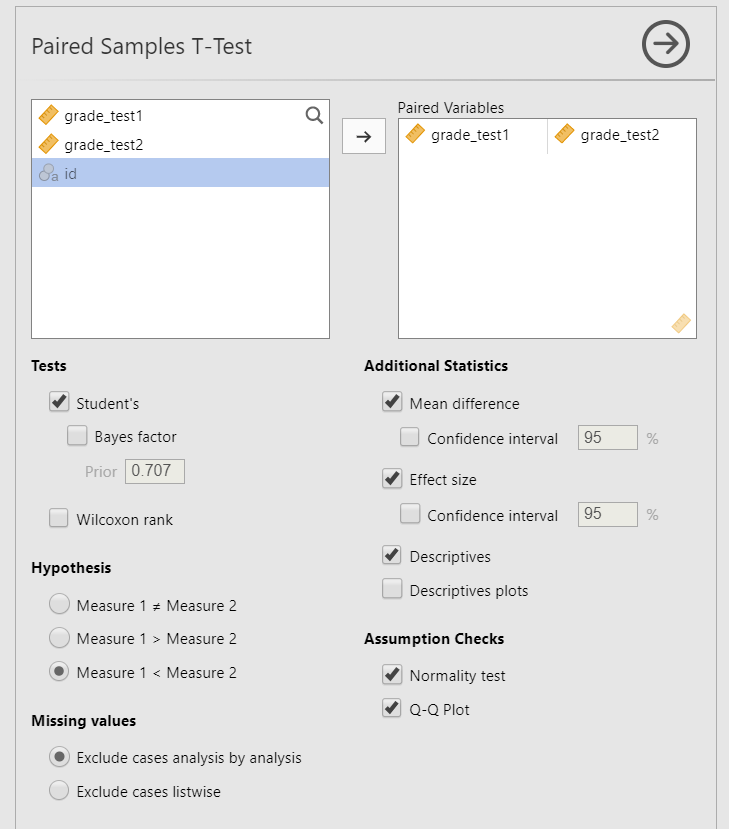
\includegraphics[width=0.8\linewidth]{images/03_dependent_t-test/dependent_setup} 

}

\caption{Dependent t-test setup in jamovi}\label{fig:unnamed-chunk-6}
\end{figure}

\hypertarget{interpreting-results}{%
\subsection{Interpreting results}\label{interpreting-results}}

Once we are satisfied we have satisfied the assumptions for the dependent t-test, we can interpret our results.

\begin{figure}

{\centering 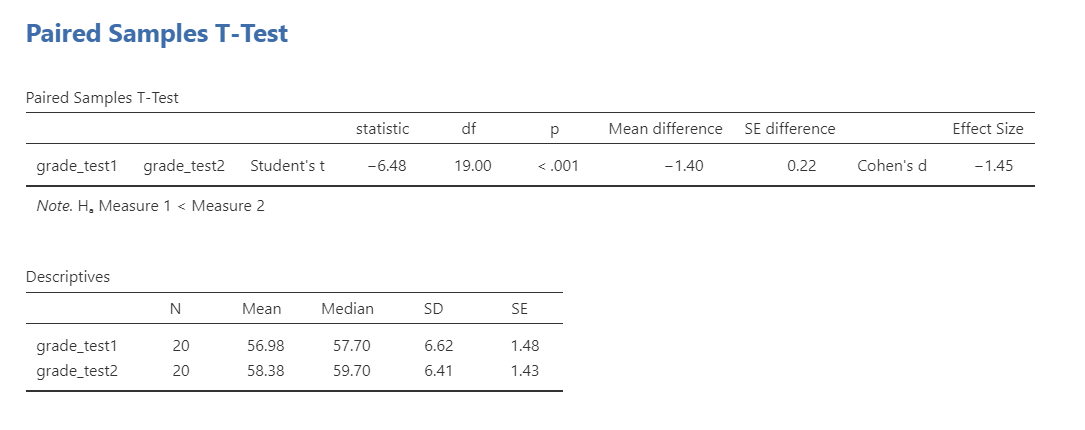
\includegraphics[width=1\linewidth]{images/03_dependent_t-test/dependent_results} 

}

\caption{Dependent t-test results in jamovi}\label{fig:unnamed-chunk-7}
\end{figure}

Our p-value is less than .05, so our results are statistically significant. Therefore, we reject the null hypothesis that there is no difference between the two groups.

\hypertarget{write-up-the-results-in-apa-style-2}{%
\subsubsection{Write up the results in APA style}\label{write-up-the-results-in-apa-style-2}}

When writing up the results of a statistical test, we should always include the following information:

\begin{enumerate}
\def\labelenumi{\arabic{enumi}.}
\tightlist
\item
  Description of your research question.
\item
  Description of your data. If you fail to meet assumptions, you should specify that and describe what test you chose to perform as a result.
\item
  The results of the inferential test, including what test was performed, the test value and degrees of freedom, p-value, and effect size.
\item
  Interpretation of the results, including any other information as needed.
\end{enumerate}

We can write up our results in APA something like this:

\begin{quote}
Dr.~Chico tested whether students performed better on the second test compared to the first test. The 20 students in performed better on the second test (\emph{M} = 58.38, \emph{SD} = 6.41) than they did on the first test (\emph{M} = 56.98, \emph{SD} = 6.62), \emph{t}(19) = 6.48, \emph{p} \textless{} .001, \emph{d} = 1.45.
\end{quote}

Remember in the previous chapter that our t-test can be negative but we can always flip the interpretation.

\hypertarget{visualize-the-results-2}{%
\subsubsection{Visualize the results}\label{visualize-the-results-2}}

By selecting \texttt{Descriptives\ plots} in the setup, you get the figure below. Personally, I don't think this is a very good plot. It's not very informative. It just provides the mean (circle), 95\% confidence interval (blue bars), and the median.

\begin{figure}

{\centering 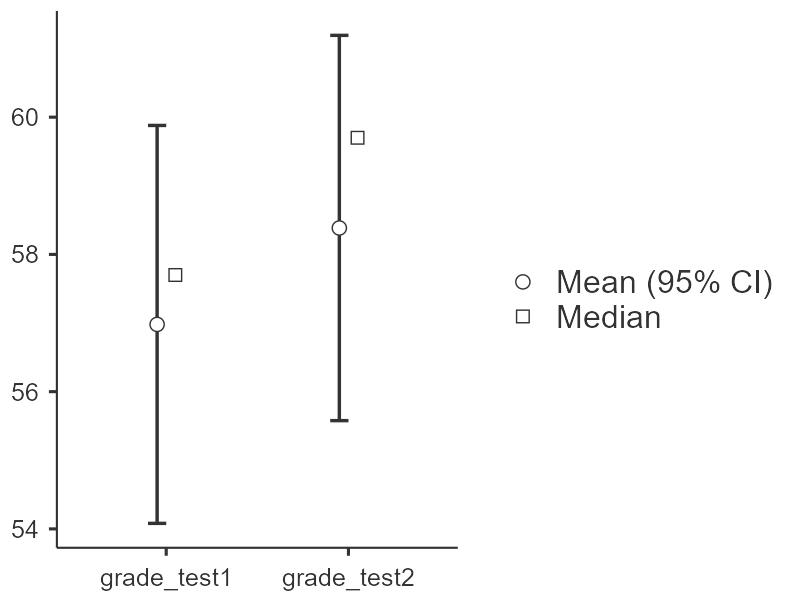
\includegraphics[width=1\linewidth]{images/03_dependent_t-test/dependent_results_plot} 

}

\caption{Dependent t-test descriptives plot}\label{fig:unnamed-chunk-8}
\end{figure}

Another option is to use the Descriptives plots available in jamovi, which we see above in the Look at the data section above. I wish there were a way to combine them into one graph, but unfortunately there isn't within jamovi. Instead, you'll have to go into the Rj editor and use R code to reshape the data from wide format to long format and then call the descriptives syntax to produce the plot. You \emph{could} copy-paste the data into a new dataset, but I always try to avoid manual work when doing analyses because something \emph{always} goes wrong.

Here's what this looks like in jamovi:

\begin{figure}

{\centering 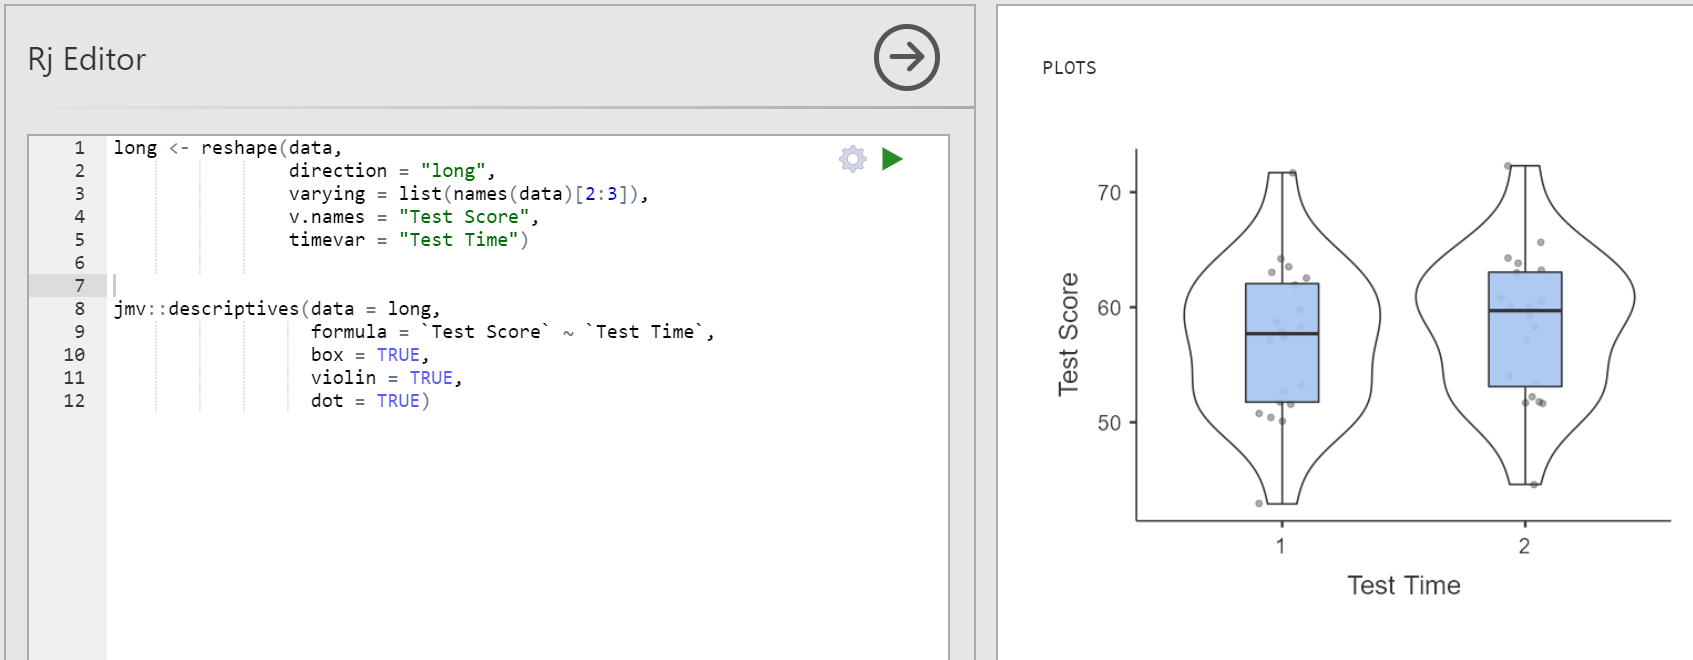
\includegraphics[width=1\linewidth]{images/03_dependent_t-test/dependent_results_plot2} 

}

\caption{Revised plot using the Rj editor}\label{fig:unnamed-chunk-9}
\end{figure}

To make our lives a bit easier, here is the code in the Rj editor that you can copy-paste (that kind of copy-pasting I allow!) into your own jamovi. You'll need to edit things like the list of names in line 3, the name of your DV (line 4), the name of your IV (line 5), and re-specify those names in line 9.

\begin{Shaded}
\begin{Highlighting}[]
\NormalTok{long }\OtherTok{\textless{}{-}} \FunctionTok{reshape}\NormalTok{(data, }
                \AttributeTok{direction =} \StringTok{"long"}\NormalTok{, }
                \AttributeTok{varying =} \FunctionTok{list}\NormalTok{(}\FunctionTok{names}\NormalTok{(data)[}\DecValTok{2}\SpecialCharTok{:}\DecValTok{3}\NormalTok{]),}
                \AttributeTok{v.names =} \StringTok{"Test Score"}\NormalTok{,}
                \AttributeTok{timevar =} \StringTok{"Test Time"}\NormalTok{)}


\NormalTok{jmv}\SpecialCharTok{::}\FunctionTok{descriptives}\NormalTok{(}\AttributeTok{data =}\NormalTok{ long,}
                  \AttributeTok{formula =} \StringTok{\textasciigrave{}}\AttributeTok{Test Score}\StringTok{\textasciigrave{}} \SpecialCharTok{\textasciitilde{}} \StringTok{\textasciigrave{}}\AttributeTok{Test Time}\StringTok{\textasciigrave{}}\NormalTok{,}
                  \AttributeTok{box =} \ConstantTok{TRUE}\NormalTok{,}
                  \AttributeTok{violin =} \ConstantTok{TRUE}\NormalTok{,}
                  \AttributeTok{dot =} \ConstantTok{TRUE}\NormalTok{)}
\end{Highlighting}
\end{Shaded}

\hypertarget{in-case-of-violated-assumptions-2}{%
\subsection{In case of violated assumptions}\label{in-case-of-violated-assumptions-2}}

If you violated the assumption of normality and no transformation fixed your data, then you can perform the non-parametric version of the dependent t-test called the Wilcoxon Rank test. As a reminder, non-parametric tests do not make assumptions about the distribution of data because it deals with the \emph{median} not the \emph{mean}.

Here is the output for both the dependent t-test and the Wilcoxon rank test:

\begin{figure}

{\centering 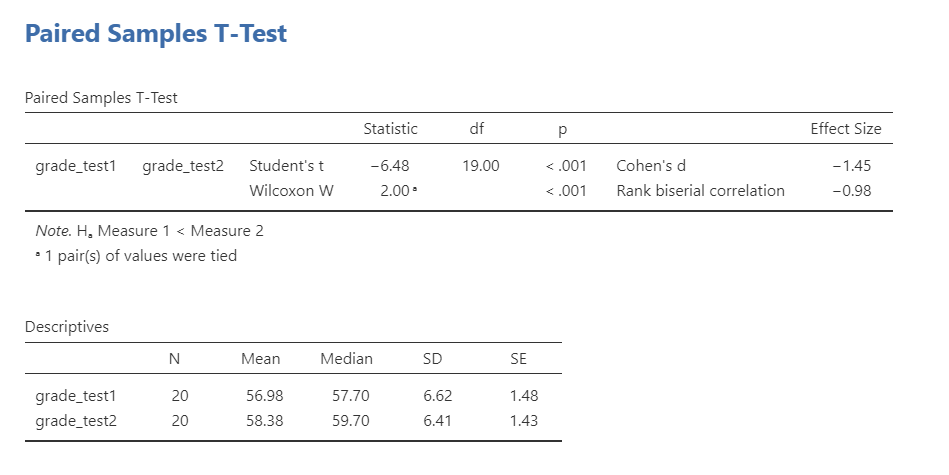
\includegraphics[width=1\linewidth]{images/03_dependent_t-test/dependent_results_full} 

}

\caption{All dependent t-test results in jamovi}\label{fig:unnamed-chunk-11}
\end{figure}

\hypertarget{wilcoxon-rank}{%
\subsubsection{Wilcoxon rank}\label{wilcoxon-rank}}

To conduct this in jamovi, under Tests select \texttt{Wilcoxon\ rank}. You will interpret the results similarly to the dependent t-test:

\begin{quote}
Using Wilcoxon rank test, students' test scores were significantly higher at the second test (\emph{Mdn} = 59.70) than at the first test (\emph{Mdn} = 57.70), W = 2.00, \emph{p} \textless{} .001.
\end{quote}

The note about tied values is not necessary to discuss. It is just telling us one participant had identical values for both test1 and test2 (student15). You can check this yourself in the dataset

\hypertarget{your-turn-2}{%
\subsection{Your turn!}\label{your-turn-2}}

Open the \texttt{Sample\_Dataset\_2014.xlsx} file that we will be using for all Your Turn exercises. You can find the dataset here: \href{https://github.com/danawanzer/stats-with-jamovi/blob/master/data/Sample_Dataset_2014.xlsx}{Sample\_Dataset\_2014.xlsx Download}

Perform dependent t-tests based on the following research questions. Think critically about whether you should be using a one-tailed or two-tailed hypothesis and check your assumptions so you know which test to use!

To get the most out of these exercises, try to first find out the answer on your own and then use the drop-down menus to check your answer.

\textbf{Note}: Technically, none of our data is suitable for a dependent t-test in this dataset. We will pretend that the four test score variables (\texttt{English}, \texttt{Reading}, \texttt{Math}, and \texttt{Writing}) are really four measurements of the same underlying test. In reality, we would analyze this data using correlation.

\begin{enumerate}
\def\labelenumi{\arabic{enumi}.}
\item
  \textbf{Do students perform better on the English test than they do the Writing test?}

  \begin{itemize}
  \item
    Should you use a one-tailed or two-tailed hypothesis? one-tailed two-tailed
  \item
    Which statistic should you use based on your assumptions? dependent t-test Wilcoxon rank
  \item
    Do students perform better on the English test than they do the Writing test? yes no
  \end{itemize}
\item
  \textbf{Does students' English scores relate to their Reading scores?}

  \begin{itemize}
  \item
    Should you use a one-tailed or two-tailed hypothesis? one-tailed two-tailed
  \item
    Which statistic should you use based on your assumptions? dependent t-test Wilcoxon rank
  \item
    Does students' English scores relate to their Reading scores? yes no
  \end{itemize}
\end{enumerate}

\hypertarget{chi-square}{%
\chapter{Chi-Square}\label{chi-square}}

The chi-quare is a categorical data analysis which is simply data analysis with categorical data. It's usually nominal data, although there are a couple tests we may use with ordinal data. There are two basic types of chi-square tests we'll be covering:

\begin{enumerate}
\def\labelenumi{\arabic{enumi}.}
\item
  \(\chi^2\) \textbf{goodness-of-fit}: used with one variable to find if the observed frequencies match the expected frequencies
\item
  \(\chi^2\) \textbf{test of independence (or association)}: used with two variables to find if the observed frequencies match the expected frequencies. In other words, are the two nominal variables independent or associated with one another?

  \begin{enumerate}
  \def\labelenumii{\arabic{enumii}.}
  \item
    \textbf{Fisher's exact test}: This is an alternative to the \(\chi^2\)test of independence that we use when our frequencies are small.
  \item
    \textbf{McNemar's test}: This is an alternative to the \(\chi^2\)test of independence that we have a 2x2 repeated-measures design. For example, perhaps we examine pass/fail rates before and after a training.
  \end{enumerate}
\end{enumerate}

Notice how we don't have an assumption about a normal distribution. For that reason, these are all \emph{non-parametric statistics}.

\hypertarget{chi-square-goodness-of-fit}{%
\section{Chi-Square Goodness-of-Fit}\label{chi-square-goodness-of-fit}}

\hypertarget{overview-3}{%
\subsection{Overview}\label{overview-3}}

The \(\chi^2\) (chi-square) goodness-of-fit tests whether an observed frequency distribution of a nominal variable matches an expected frequency distribution. Our hypotheses for the chi-square goodness-of-fit test is as follows:

\begin{itemize}
\item
  \(H_0\): The observed frequencies match the expected frequencies.
\item
  \(H_1\): At least one observed frequency doesn't match the expected frequency.
\end{itemize}

For example, if we have a deck of cards and want to see if people don't choose cards randomly, the null hypothesis would be that there is a 25\% probability of getting each hearts, clubs, spades, and diamonds.

\hypertarget{look-at-the-data-3}{%
\subsection{Look at the data}\label{look-at-the-data-3}}

\hypertarget{data-set-up-3}{%
\subsubsection{Data set-up}\label{data-set-up-3}}

Our data set-up for a chi-square goodness-of-fit test is pretty simple, We just need a single column with the nominal category that each participant is in.

\hypertarget{describe-your-data}{%
\subsubsection{Describe your data}\label{describe-your-data}}

\hypertarget{check-assumptions-3}{%
\subsection{Check assumptions}\label{check-assumptions-3}}

The chi-square goodness-of-fit test has the following assumptions:

\begin{enumerate}
\def\labelenumi{\arabic{enumi}.}
\item
  \textbf{Expected frequencies are sufficiently large}, which is usually greater than 5. If you violate this assumption, you can use Fisher's exact test.
\item
  Data are independent of one another, meaning each case contributes to only one cell of the table. If you violate this assumption, you may be able to use the McNemar test.
\end{enumerate}

\hypertarget{perform-the-test-3}{%
\subsection{Perform the test}\label{perform-the-test-3}}

Let's run an example with data from lsj-data. Open data from your Data Library in ``lsj-data''. Select and open ``randomness''. This dataset has participants pull two cards from a deck. For now, let's just work with \texttt{choice\_1}.

\begin{enumerate}
\def\labelenumi{\arabic{enumi}.}
\item
  From the `Analyses' toolbar select `Frequences' - `One sample proportion tests - N outcomes'.
\item
  Move \texttt{choice\_1} into the Variable box.
\item
  Select \texttt{Expected\ counts}.
\end{enumerate}

When you are done, your setup should look like this

\begin{figure}

{\centering 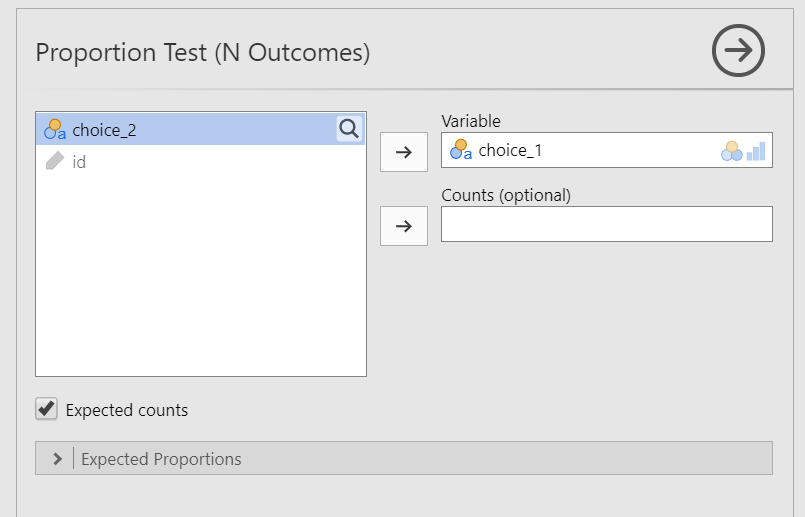
\includegraphics[width=0.8\linewidth]{images/09-chi-square/chi-square_setup} 

}

\caption{Chi-square goodness-of-fit setup in jamovi}\label{fig:unnamed-chunk-1}
\end{figure}

\hypertarget{interpret-results-2}{%
\subsection{Interpret results}\label{interpret-results-2}}

\begin{figure}

{\centering 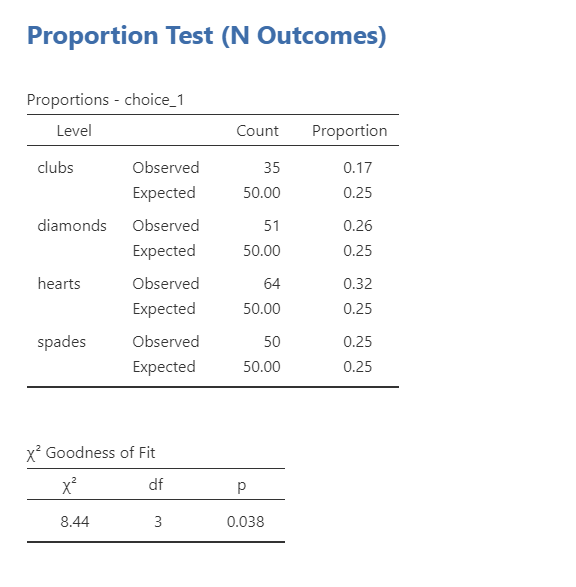
\includegraphics[width=1\linewidth]{images/09-chi-square/chi-square_results} 

}

\caption{Chi-square goodness-of-fit results in jamovi}\label{fig:unnamed-chunk-2}
\end{figure}

The first table shows us our observed frequencies (our data) and expected frequencies (N/k = 200/4 = 50). The second table gives us our results. Our p-value is less than .05 so we can reject the null hypothesis that the observed frequencies match our expected frequencies.

\hypertarget{write-up-the-results-in-apa-style-3}{%
\subsubsection{Write up the results in APA style}\label{write-up-the-results-in-apa-style-3}}

We can write up our results in APA something like this:

\begin{quote}
Of the 200 participants in the experiment, 64 selected hearts for their first choice, 51selected diamonds, 50 selected spades, and 35 selected clubs. A chi-square goodness-of-fit test was conducted to test whether the choice probabilities were identical for all four suits. The results were statistically significant (\(\chi^2\) (3) = 8.44; \emph{p} = .038), suggesting that people did not select suits purely at random.
\end{quote}

\hypertarget{visualize-the-results-3}{%
\subsubsection{Visualize the results}\label{visualize-the-results-3}}

\hypertarget{additional-information-1}{%
\subsection{Additional information}\label{additional-information-1}}

\hypertarget{different-expected-frequencies}{%
\subsubsection{Different Expected Frequencies}\label{different-expected-frequencies}}

As you can tell, jamovi automatically assumed equal proportions of frequencies. However, perhaps we think our deck is loaded or we have the actual population frequencies and want to see if our distribution matches the population distribution. We can use the \texttt{Expected\ Proportions} in the setup to specify different expected frequencies.

For example, maybe we think our deck is a little stacked in favor of red cards--or we think our participants are more likely to choose red cards than black cards. We can specify our expected proportions and then interpret the results. In this case, participants do not seem more likely to choose red cards based on the expected frequencies we provided.

\begin{figure}

{\centering 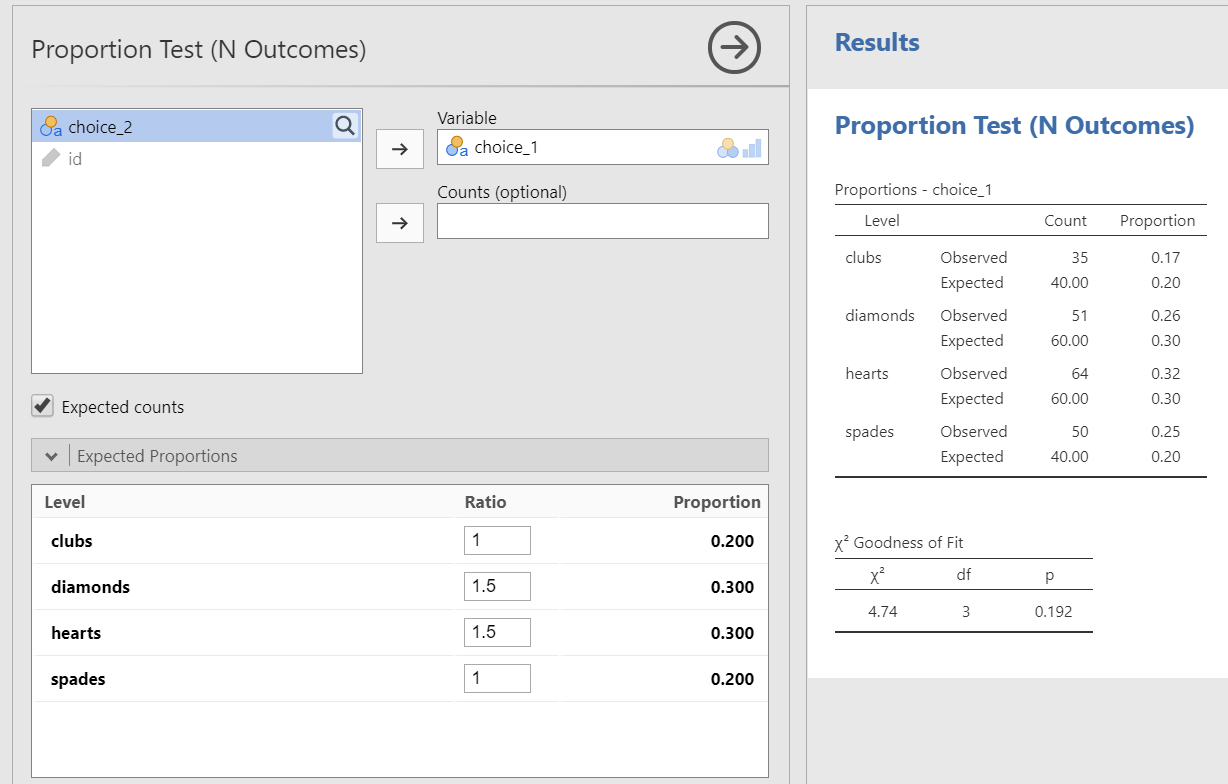
\includegraphics[width=1\linewidth]{images/09-chi-square/chi-square_results2} 

}

\caption{Chi-square goodness-of-fit - Different expected proportions}\label{fig:unnamed-chunk-3}
\end{figure}

\hypertarget{your-turn-3}{%
\subsection{Your turn!}\label{your-turn-3}}

Open the \texttt{Sample\_Dataset\_2014.xlsx} file that we will be using for all Your Turn exercises. You can find the dataset here: \href{https://github.com/danawanzer/stats-with-jamovi/blob/master/data/Sample_Dataset_2014.xlsx}{Sample\_Dataset\_2014.xlsx Download}

To get the most out of these exercises, try to first find out the answer on your own and then use the drop-down menus to check your answer.

\begin{enumerate}
\def\labelenumi{\arabic{enumi}.}
\item
  \textbf{Are there equal numbers of athletes and non-athletes?} (\texttt{Athlete} variable)

  \begin{itemize}
  \item
    Do you meet the assumptions? yes no, expected frequencies are too small no, data are not independent
  \item
    Are the observed frequencies similar to the expected frequencies? yes no
  \item
    What is your chi-square value, rounded to two decimal places:
  \end{itemize}
\item
  \textbf{I happen to know the school this data comes from has 40\% athletes and 60\% non-athletes. Does our data match the school population?}

  \begin{itemize}
  \item
    Change your Expected Proportions ratio to .6 for non-athletes and .4 for athletes.
  \item
    Are the observed frequencies similar to the expected frequencies? yes no
  \item
    What is your chi-square value, rounded to two decimal places:
  \end{itemize}
\item
  \textbf{Are there equal numbers of freshmen, sophomores, juniors, and seniors?} (\texttt{Rank} variable)

  \begin{itemize}
  \item
    Do you meet the assumptions? yes no, expected frequencies are too small no, data are not independent
  \item
    Are the observed frequencies similar to the expected frequencies? yes no
  \item
    What is your chi-square value, rounded to two decimal places:
  \end{itemize}
\end{enumerate}

\hypertarget{chi-square-test-of-independence}{%
\section{Chi-Square Test of Independence}\label{chi-square-test-of-independence}}

\hypertarget{overview-4}{%
\subsection{Overview}\label{overview-4}}

The \(\chi^2\) (chi-square) test of independence (or association) tests whether an observed frequency distribution of a nominal variable matches an expected frequency distribution, but unlike the goodness of fit test we are looking at the relationship, independence, or association between two variables. Our hypotheses for the chi-square goodness-of-fit test is as follows:

\begin{itemize}
\item
  \(H_0\): The observed frequencies match the expected frequencies.
\item
  \(H_1\): At least one observed frequency doesn't match the expected frequency.
\end{itemize}

For example, imagine we are watching a show about the planet \emph{Chapek 9}. On this planet, for someone to gain access to their capital city they must prove they're a robot, not a human. In order to determine whether or not a visitor is human, the natives ask whether the visitor prefers puppies, flowers, or large, properly formatted data files. Our alternative hypothesis would be that humans and robots have different preferences and our null is that they have the same preferences.

\hypertarget{look-at-the-data-4}{%
\subsection{Look at the data}\label{look-at-the-data-4}}

\hypertarget{data-set-up-4}{%
\subsubsection{Data set-up}\label{data-set-up-4}}

Our data set-up for a chi-square test of independence is pretty simple, We just need two columns of nominal data, with one row per participant. Here's our data for our example we'll be working with, which you can find in the lsj-data called \texttt{chapek9}:

\begin{longtable}[]{@{}lll@{}}
\toprule
ID & species & choice\tabularnewline
\midrule
\endhead
1 & robot & flower\tabularnewline
2 & human & data\tabularnewline
3 & human & data\tabularnewline
4 & human & data\tabularnewline
5 & robot & data\tabularnewline
6 & human & flower\tabularnewline
7 & human & data\tabularnewline
8 & robot & data\tabularnewline
9 & human & puppy\tabularnewline
10 & robot & flower\tabularnewline
\bottomrule
\end{longtable}

\hypertarget{describe-the-data-3}{%
\subsubsection{Describe the data}\label{describe-the-data-3}}

\hypertarget{check-assumptions-4}{%
\subsubsection{Check assumptions}\label{check-assumptions-4}}

\hypertarget{perform-the-test-4}{%
\subsection{Perform the test}\label{perform-the-test-4}}

Let's run an example with data from lsj-data. Open data from your Data Library in ``lsj-data''. Select and open ``chapek9''. This dataset indicates the ID number of the participant, the species (robot or human), and their preference of the three things (puppy, flower, or data).

\begin{enumerate}
\def\labelenumi{\arabic{enumi}.}
\item
  From the `Analyses' toolbar select `Frequencies' - `Independent Samples - \(\chi^2\) test of association'.
\item
  Move \texttt{choice} into rows and \texttt{species} into columns. Note that the placement in rows or columns doesn't really matter, but because we typically work with portrait pages I tend to prefer putting in rows whatever variable has more levels. In this case, choice has 3 levels and species only 2 so I like to put choice in rows and species in columns.
\item
  Under the Statistics tab, select \(\chi^2\) under Tests and \texttt{Phi\ and\ Cramer\textquotesingle{}s\ V} under Nominal.
\item
  Optionally, you can request under the Cells tab to show the expected counts and the row, column, and total percentages.
\end{enumerate}

When you are done, your setup should look like this

\begin{figure}

{\centering 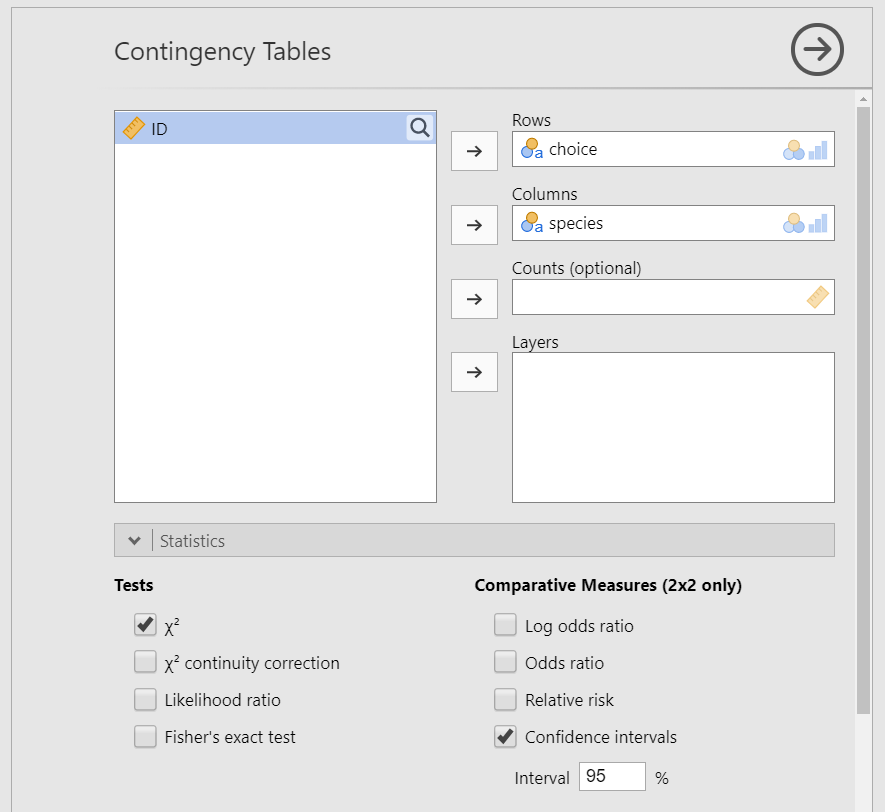
\includegraphics[width=0.8\linewidth]{images/11-independence/independence_setup} 

}

\caption{Chi-square test of independence setup in jamovi}\label{fig:unnamed-chunk-1}
\end{figure}

\hypertarget{interpreting-results-1}{%
\subsection{Interpreting results}\label{interpreting-results-1}}

\begin{figure}

{\centering 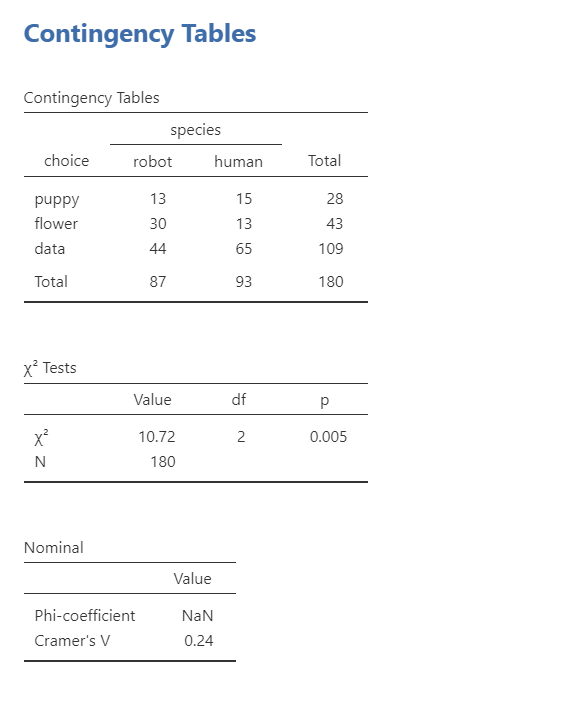
\includegraphics[width=1\linewidth]{images/11-independence/independence_results} 

}

\caption{Chi-square test of independence results in jamovi}\label{fig:unnamed-chunk-2}
\end{figure}

The first table shows us our observed frequencies. The second table gives us our results. Our p-value is less than .05 so we can reject the null hypothesis that the observed frequencies match our expected frequencies. jamovi also gives us our Cramer's V value.

\hypertarget{write-up-the-results-in-apa-style-4}{%
\subsubsection{Write up the results in APA style}\label{write-up-the-results-in-apa-style-4}}

We can write up our results in APA something like this:

\begin{quote}
Pearson's \(\chi^2\) test of independence showed a significant association between species and choice, \(\chi^2\) (2) = 10.72, \emph{p} = .005, Cramer's V = .24. Robots appeared to be more likely to say they prefer flowers and humans appeared to be more likely to say they prefer data.
\end{quote}

I would either write-up the observed frequencies above or, ideally, I would share the contingency table with my observed frequencies.

\hypertarget{visualize-the-results-4}{%
\subsubsection{Visualize the results}\label{visualize-the-results-4}}

\hypertarget{in-case-of-violated-assumptions-3}{%
\subsection{In case of violated assumptions}\label{in-case-of-violated-assumptions-3}}

\hypertarget{fishers-exact-test}{%
\subsubsection{Fisher's exact test}\label{fishers-exact-test}}

If you violate the assumption that there your expected frequencies are sufficiently large and you have a 2x2 table, you can still perform the \(\chi^2\) test of independence but instead of selecting \(\chi^2\)you'll select \texttt{Fisher\textquotesingle{}s\ exact\ test}. You'll interpret your results exactly the same but specify you used the Fisher's exact test.

\hypertarget{additional-information-2}{%
\subsection{Additional information}\label{additional-information-2}}

\hypertarget{ordinal-variables}{%
\subsubsection{Ordinal variable(s)}\label{ordinal-variables}}

If either of your variables are ordinal, instead of selecting \texttt{Phi\ and\ Cramer\textquotesingle{}s\ V} you should select \texttt{Gamma} or \texttt{Kendall\textquotesingle{}s\ tau-b}. Which do you choose? \texttt{Kendall\textquotesingle{}s\ tau-b} should only be chosen if you have a square table (e.g., 3x3, 4x4, 5x5) whereas \texttt{Gamma} can be done with any size table. \texttt{Kendall\textquotesingle{}s\ tau-b} will be a slightly more conservative estimate compared to \texttt{Gamma}.

\hypertarget{your-turn-4}{%
\section{Your turn!}\label{your-turn-4}}

Open the \texttt{Sample\_Dataset\_2014.xlsx} file that we will be using for all Your Turn exercises. You can find the dataset here: \href{https://github.com/danawanzer/stats-with-jamovi/blob/master/data/Sample_Dataset_2014.xlsx}{Sample\_Dataset\_2014.xlsx Download}

To get the most out of these exercises, try to first find out the answer on your own and then use the drop-down menus to check your answer.

\begin{enumerate}
\def\labelenumi{\arabic{enumi}.}
\item
  \textbf{Is Athlete related to Gender?}

  \begin{itemize}
  \item
    Do you meet the assumptions? yes no, expected frequencies are too small no, data are not independent
  \item
    Which test should you perform? Chi-square Fisher's exact test
  \item
    Are the observed frequencies similar to the expected frequencies? yes no
  \item
    What is your chi-square value, rounded to two decimal places:
  \end{itemize}
\item
  \textbf{Is Gender related to Rank?}

  \begin{itemize}
  \item
    Do you meet the assumptions? yes no, expected frequencies are too small no, data are not independent
  \item
    Which test should you perform? Chi-square Fisher's exact test
  \item
    Are the observed frequencies similar to the expected frequencies? yes no
  \item
    What is your chi-square value, rounded to two decimal places:
  \end{itemize}
\end{enumerate}

\hypertarget{mcnemars-test}{%
\section{McNemar's Test}\label{mcnemars-test}}

\hypertarget{overview-5}{%
\subsection{Overview}\label{overview-5}}

McNemar's test is based on the \(\chi^2\) (chi-square) test of independence (or association), but is used in a repeated measures or within-subjects design. Our hypotheses for the McNemar test is as follows:

\begin{itemize}
\item
  \(H_0\): The observed frequencies match the expected frequencies.
\item
  \(H_1\): At least one observed frequency doesn't match the expected frequency.
\end{itemize}

For example, suppose we're working with the \emph{Australian Generic Political Party} (AGPP) and your job is to find out how effective AGPP political advertisements are. You gather 100 people and ask them to watch the AGPP ads. You ask participants before and after viewing ads whether they intend to vote for the AGPP.

\hypertarget{look-at-the-data-5}{%
\subsection{Look at the data}\label{look-at-the-data-5}}

\hypertarget{data-set-up-5}{%
\subsubsection{Data set-up}\label{data-set-up-5}}

Our data set-up for McNemar's test is pretty simple. We just need two columns of nominal data, with one row per participant and each column being the same variable at two different time points. Here's our data for our example we'll be working with, which you can find in the lsj-data called \texttt{agpp}:

\begin{longtable}[]{@{}lll@{}}
\toprule
ID & response\_before & response\_after\tabularnewline
\midrule
\endhead
subj.1 & no & yes\tabularnewline
subj.2 & yes & no\tabularnewline
subj.3 & yes & no\tabularnewline
subj.4 & yes & no\tabularnewline
subj.5 & no & no\tabularnewline
subj.6 & no & no\tabularnewline
subj.7 & no & no\tabularnewline
subj.8 & no & yes\tabularnewline
subj.9 & no & no\tabularnewline
subj.10 & no & no\tabularnewline
\bottomrule
\end{longtable}

\hypertarget{describe-the-data-4}{%
\subsubsection{Describe the data}\label{describe-the-data-4}}

\hypertarget{perform-the-test-5}{%
\subsection{Perform the test}\label{perform-the-test-5}}

Let's run an example with data from lsj-data. Open data from your Data Library in ``lsj-data''. Select and open ``agpp''. This dataset indicates the ID number of the participant and whether they would vote for AGPP before and after viewing the ads.

\begin{enumerate}
\def\labelenumi{\arabic{enumi}.}
\item
  From the `Analyses' toolbar select `Frequencies' - `Paired Samples - McNemar test'.
\item
  Move \texttt{response\_before} into rows and \texttt{response\_after} into columns. Note that the placement in rows or columns doesn't really matter.
\item
  Under the Statistics tab, select \(\chi^2\) under Tests.
\item
  Optionally, you can request under to show the row and column percentages.
\end{enumerate}

When you are done, your setup should look like this

\begin{figure}

{\centering 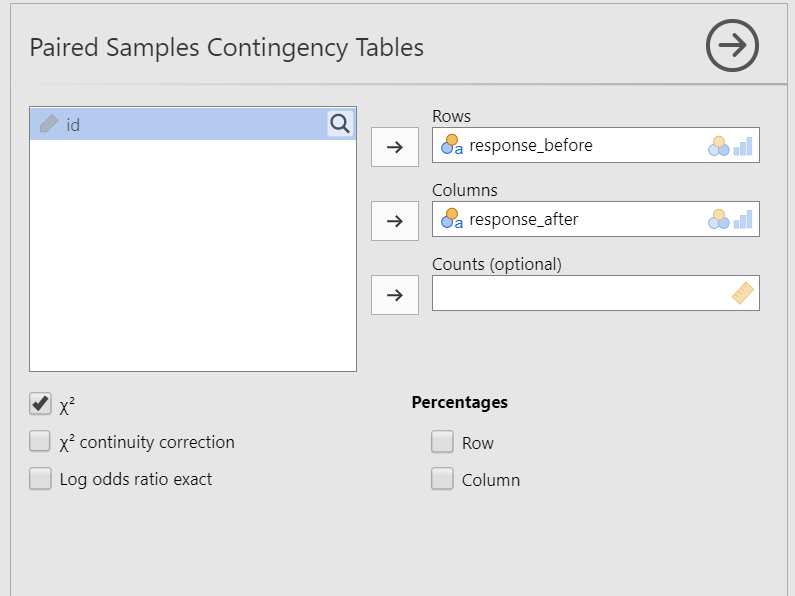
\includegraphics[width=0.8\linewidth]{images/12-mcnemar/mcnemar_setup} 

}

\caption{McNemar's test setup in jamovi}\label{fig:unnamed-chunk-1}
\end{figure}

\hypertarget{interpret-results-3}{%
\subsection{Interpret results}\label{interpret-results-3}}

\begin{figure}

{\centering 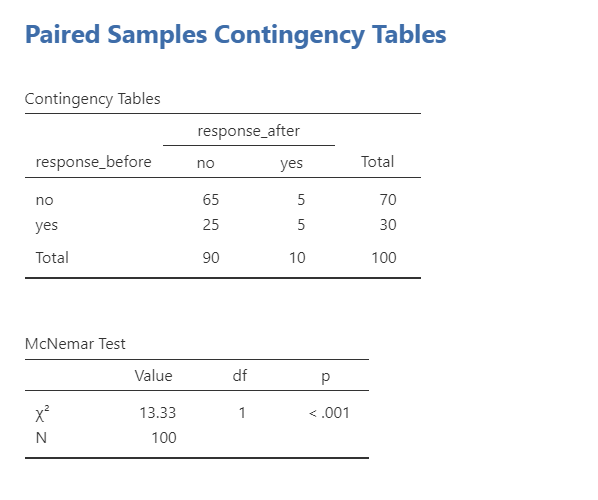
\includegraphics[width=1\linewidth]{images/12-mcnemar/mcnemar_results} 

}

\caption{McNemar's test results in jamovi}\label{fig:unnamed-chunk-2}
\end{figure}

The first table shows us our observed frequencies. The second table gives us our results. Our p-value is less than .05 so we can reject the null hypothesis that the observed frequencies match our expected frequencies. Unfortunately, looking at our table it also shows that the ads had a negative effect: people were less likely to vote AGPP after seeing the ads.

\hypertarget{write-up-the-results-in-apa-style-5}{%
\subsubsection{Write up the results in APA style}\label{write-up-the-results-in-apa-style-5}}

We can write up our results in APA something like this:

\begin{quote}
McNemar's test indicated that support for AGPP changed from before to after reviewing the AGPP advertisement, \(\chi^2\) (1) = 13.33, \emph{p} \textless{} .001. Most participants continued to not vote for AGPP after the ad (\emph{n} = 65) and a few continued to vote for AGPP after the ad (\emph{n} = 5). However, many participants who originally stated they would vote for AGPP changed to no longer voting for AGPP after the ad (\emph{n} = 25); only five people who originally would not vote for AGPP changed to vote for AGPP after the ad.
\end{quote}

\hypertarget{visualize-the-results-5}{%
\subsubsection{Visualize the results}\label{visualize-the-results-5}}

\hypertarget{anova}{%
\chapter{ANOVA}\label{anova}}

ANOVA stands for \textbf{AN}alysis \textbf{O}f \textbf{VA}riance. ANOVAs analyze the variation between and within groups. There are multiple types of ANOVAs based on the nature of the independent variable(s):

\begin{longtable}[]{@{}ll@{}}
\toprule
\textbf{Nature of IV(s)} & \textbf{Type of ANOVA}\tabularnewline
\midrule
\endhead
1 between-subjects IV & One-way ANOVA\tabularnewline
1 within-subjects IV & Repeated-measures ANOVA\tabularnewline
2+ between-subjects IVs & Independent factorial ANOVA\tabularnewline
2+ within-subjects IVs & Repeated measures factorial ANOVA\tabularnewline
2+ IVs mixed between/within & Mixed factorial ANOVA\tabularnewline
1+ IV with a continuous covariate & ANCOVA\tabularnewline
\bottomrule
\end{longtable}

Furthermore, there are ANOVAs for when there are multiple dependent variables (called the MANOVA or \textbf{M}ultiple \textbf{ANOVA}, as well as the MANCOVA or \textbf{M}ultiple \textbf{ANCOVA}) but we will not discuss them in this class.

\hypertarget{one-way-anova}{%
\section{One-way ANOVA}\label{one-way-anova}}

\hypertarget{overview-6}{%
\subsection{Overview}\label{overview-6}}

The one-way analysis of variance (ANOVA) is used to test the difference in our dependent variable between \underline{three or more} different groups of observations. Our grouping variable is our independent variable. In other words, we use the one-way ANOVA when we have a research question with a \textbf{continuous dependent variable} and a \textbf{categorical independent variable with three or more categories in which different participants are in each category}.

The one-way ANOVA is also known as an independent factor ANOVA.

One thing to keep in mind is the one-way ANOVA is an omnibus statistic that tests against the null hypothesis that the three or more means are the same. It does not tell us where the mean differences are (e.g., that 1 \textgreater{} 2); for that, we need planned contrasts or post-hoc procedures, which you'll learn about later. Therefore, the null and alternative hypotheses for the one-way ANOVA are as follows:

\begin{itemize}
\tightlist
\item
  \(H_0\): There is \textbf{no difference} in means between the groups. In other words, the means for the three or more groups are the \textbf{same}.
\item
  \(H_1\): There is \textbf{a difference} in means between the groups. In other words, the means for the three or more groups are \textbf{different}.
\end{itemize}

\hypertarget{why-not-multiple-t-tests}{%
\subsubsection{Why not multiple t-tests?}\label{why-not-multiple-t-tests}}

In the example above, we have three groups: fall, spring, and summer. We could just perform three separate t-tests: fall vs.~spring, fall vs.~summer, and spring vs.~summer.

However, the reason we do not perform multiple t-tests is to reduce our Type I error rate. If I had performed three separate t-tests, set my alpha (Type I error rate) at 5\%, and knew for a fact the effects do not actually exist, then each test has a probability of a Type I error rate of 5\%. Because we are running three tests, our alpha rate actually becomes 1 - (.95\textsuperscript{3})= 1 - .857 = 14.3\%! So now our \emph{familywise} or \emph{experimentwise} error rate is 14.3\%, not the 5\% we originally set alpha at.

With three groups, that's not so bad, but let's see what happens with more tests we perform:

\begin{itemize}
\tightlist
\item
  \textbf{1 test}: 1 - (.95\textsuperscript{1})= 1 - .95 = \textbf{5\%}
\item
  \textbf{2 tests}: 1 - (.95\textsuperscript{2})= 1 - .9025 = \textbf{9.8\%}
\item
  \textbf{3 tests}: 1 - (.95\textsuperscript{3})= 1 - .857 = \textbf{14.3\%}
\item
  \textbf{4 tests}: 1 - (.95\textsuperscript{4})= 1 - .814 = \textbf{18.6\%}
\item
  \textbf{5 tests}: 1 - (.95\textsuperscript{5})= 1 - .774 = \textbf{22.6\%}
\item
  \textbf{10 tests}: 1 - (.95\textsuperscript{10})= 1 - .598 = \textbf{40.1\%}
\item
  \textbf{20 tests}: 1 - (.95\textsuperscript{20})= 1 - .358 = \textbf{64.1\%}
\end{itemize}

Ouch! 10 tests would have a Type I error rate of 40\%! That means that if we performed 10 statistical tests (assuming the effect does not exist), then 40\% of the results would be statistically significant by chance alone and would be a false positive. That's not good!

Therefore, we use the one-way ANOVA as one test to see if there is a difference overall. We can also do things to control or limit our familywise error rate, which I'll get into later.

\hypertarget{look-at-the-data-6}{%
\subsection{Look at the data}\label{look-at-the-data-6}}

DATASET INFO

\hypertarget{data-set-up-6}{%
\subsubsection{Data set-up}\label{data-set-up-6}}

To conduct the one-way ANOVA, we first need to ensure our data is set-up properly in our dataset. This requires having two columns: one with our continuous dependent variable and one indicating which group the participant is in. Each row is a unique participant or unit of analysis.

INCLUDE DATASET HERE

In the data above, what is your \textbf{independent variable}? ID Semester TestScore

In the data above, what is your \textbf{dependent variable}? ID Semester TestScore

\hypertarget{describe-the-data-5}{%
\subsubsection{Describe the data}\label{describe-the-data-5}}

\hypertarget{anova-assumptions}{%
\subsection{Check assumptions}\label{anova-assumptions}}

\hypertarget{assumptions-3}{%
\subsubsection{Assumptions}\label{assumptions-3}}

As a parametric test, the one-way ANOVA has the same assumptions as other parametric tests:

\begin{enumerate}
\def\labelenumi{\arabic{enumi}.}
\item
  The dependent variable is \textbf{normally distributed}
\item
  Variances in the two groups are roughly equal (i.e., \textbf{homogeneity of variances})
\item
  The dependent variable is \textbf{interval or ratio} (i.e., continuous)
\item
  Scores are \textbf{independent} between groups
\end{enumerate}

We cannot \emph{test} the third and fourth assumptions; rather, those are based on knowing your data.

However, we can and should test for the first two assumptions. Fortunately, the one-way ANOVA in jamovi has three check boxes under ``Assumption Checks'' that lets us test for both assumptions.

\hypertarget{anova-is-robust-to-violations}{%
\subsubsection{ANOVA is robust to violations}\label{anova-is-robust-to-violations}}

Although we should meet the assumptions as much as possible, in general the F-statistic is \emph{robust} to violations of normality and homogeneity of variance. This means that you can still run the one-way ANOVA if you violate the assumptions, but \emph{only when group sizes are equal or nearly equal}. If you have vastly different variances (such as 2:1 ratio or greater) or vastly different group sizes (such as a 2:1 ratio or greater), and especially if one group is small (such as 10 or fewer cases), then your F-statistic is likely to be very wrong. For example, if your larger group has the larger variance, then your F-statistic is likely to be non-significant or smaller than it should be; however, if your larger group has smaller variance,then your F-statistic is likely to be significant or bigger than it should be!

\hypertarget{checking-assumptions-3}{%
\subsubsection{Checking assumptions}\label{checking-assumptions-3}}

We test for normality using the Shapiro-Wilk test and the Q-Q plot. The Shapiro-Wilk test was not statistically significant (W = .96, \emph{p} = .605); therefore, this indicates the data is normally distributed. Furthermore, the lines are fairly close to the diagonal line in the Q-Q plot. We can conclude that we satisfy the assumption of normality.

We test for homogeneity of variance using the Levene's test. The Levene's test was not statistically significant (\emph{F} {[}2, 15{]} = 1.45, \emph{p} = .266); therefore, this indicates our data satisfies the assumption of homogeneity of variance. However, I would add a caveat that we have a small sample of data (\emph{N} = 18); we should have tried to collect more data.

\begin{figure}

{\centering 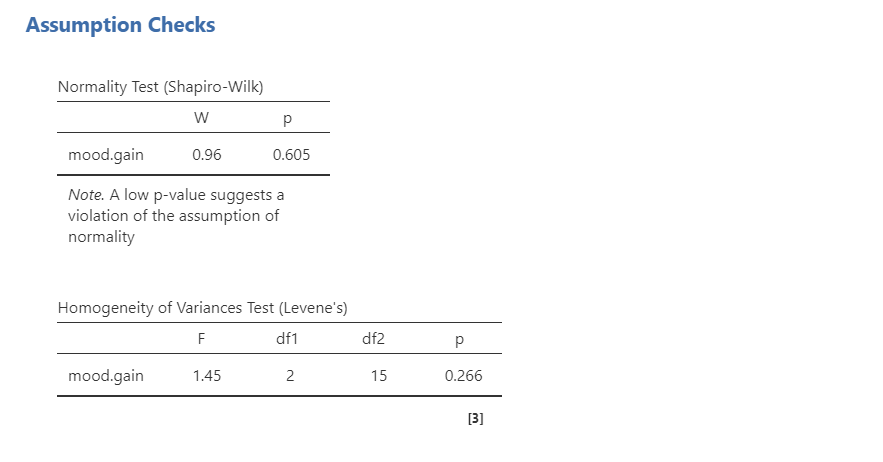
\includegraphics[width=1\linewidth]{images/04_one-way-anova/one-way_assumptions1} 

}

\caption{Testing assumptions in jamovi}\label{fig:unnamed-chunk-1}
\end{figure}

\begin{figure}

{\centering 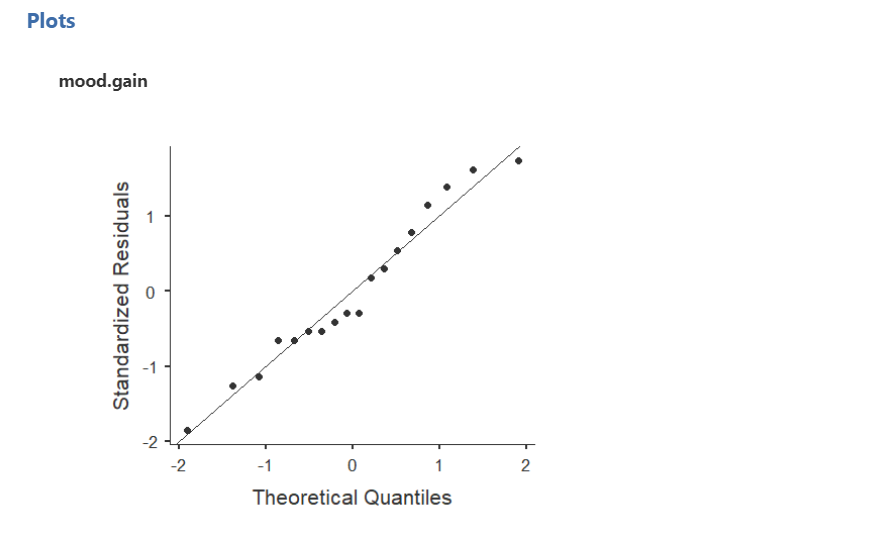
\includegraphics[width=1\linewidth]{images/04_one-way-anova/one-way_assumptions2} 

}

\caption{Testing assumptions in jamovi}\label{fig:unnamed-chunk-2}
\end{figure}

\hypertarget{perform-the-test-6}{%
\subsection{Perform the test}\label{perform-the-test-6}}

Let's run an example with data from lsj-data. Open data from your Data Library in ``lsj-data''. Select and open ``clinicaltrial''. This dataset is hypothetical data of a clinical trial in which you are testing a new antidepressant drug called \emph{Joyzepam}. In order to construct a fair test of the drug's effectiveness, the study involves three separate drugs to be administered. One is a placebo, and the other is an existing antidepressant / anti-anxiety drug called \emph{Anxifree}. A collection of 18 participants with moderate to severe depression are recruited for your initial testing. Because the drugs are sometimes administered in conjunction with psychological therapy, your study includes 9 people undergoing cognitive behavioral therapy (CBT) and 9 who are not. Participants are randomly assigned (doubly blinded, of course) a treatment, such that there are 3 CBT people and 3 no-therapy people assigned to each of the 3 drugs. A psychologist assesses the mood of each person after a 3 month run with each drug, and the overall improvement in each person's mood is assessed on a scale ranging from -5 to +5.

\textbf{Note}: Do not use the one-way ANOVA analysis in jamovi! The options there are too limited for our use. Instead, be sure you use ANOVA!

\begin{enumerate}
\def\labelenumi{\arabic{enumi}.}
\item
  To perform a one-way ANOVA in jamovi, go to the Analyses tab, click the \textbf{ANOVA} button, and choose ``ANOVA''. You might be asking why we aren't choosing ``One-Way ANOVA'' and that's because the options there are too limited.
\item
  Move your dependent variable \texttt{mood.gain} to the Dependent Variable box and your independent variable \texttt{drug} to the Fixed Factors box.
\item
  Select \(\omega^2\) (omega-squared) for your effect size.
\item
  Ignore the Model drop-down menu. If you are doing more complicated ANOVAs you will need this. We will ignore it.
\item
  In the Assumption Checks drop-down menu, select all three options: \texttt{Homogeneity\ test}, \texttt{Normality\ test}, and \texttt{Q-Q\ plot}.
\item
  Ignore the Contrasts and Post Hoc Tests drop-down menus for now. See below for more information on them.
\item
  In the Estimated Marginal Means drop-down menu, move your IV \texttt{drug} to the Marginal Means box and select \texttt{Marginal\ means\ plots}, \texttt{Marginal\ means\ tables}, and \texttt{Observed\ scores}, in addition to the pre-selected \texttt{Equal\ cell\ weights}.
\end{enumerate}

When you are done, your setup should look like this:

\begin{figure}

{\centering 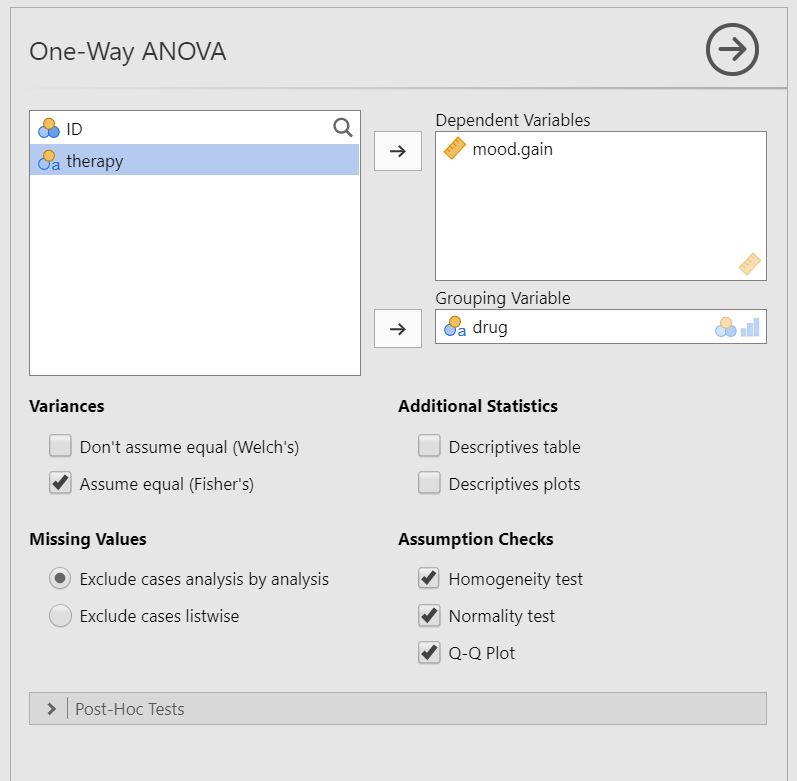
\includegraphics[width=0.8\linewidth]{images/04_one-way-anova/one-way_setup} 

}

\caption{One-way ANOVA setup in jamovi}\label{fig:unnamed-chunk-3}
\end{figure}

\hypertarget{interpret-results-4}{%
\subsection{Interpret results}\label{interpret-results-4}}

Once we are satisfied we have satisfied the assumptions for the one-way ANOVA, we can interpret our results.

\begin{figure}

{\centering 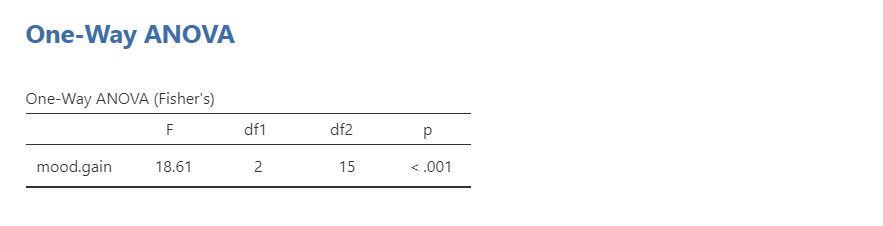
\includegraphics[width=1\linewidth]{images/04_one-way-anova/one-way_results} 

}

\caption{One-way ANOVA results in jamovi}\label{fig:unnamed-chunk-4}
\end{figure}

Our p-value is less than .05, so our results are statistically significant.

\hypertarget{write-up-the-results-in-apa-style-6}{%
\subsubsection{Write up the results in APA style}\label{write-up-the-results-in-apa-style-6}}

We can write up our results in APA something like this:

\begin{quote}
There is a significant difference in mood gain across the three drug conditions, \emph{F} (2, 15) = 18.61, \emph{p} \textless{} .001, \(\omega^2\) = .66.
\end{quote}

Sometimes, people like to put the statistics inside a parentheses. In that case, you need to change the parentheses around the degrees of freedom as brackets. Here's another example write-up of the results in APA style:

\begin{quote}
There is a significant difference in mood gain across the three drug conditions (\emph{F} {[}2, 15{]} = 18.61, \emph{p} \textless{} .001, \(\omega^2\) = .66).
\end{quote}

\hypertarget{visualize-the-results-6}{%
\subsubsection{Visualize the results}\label{visualize-the-results-6}}

\hypertarget{in-case-of-violated-assumptions-4}{%
\subsection{In case of violated assumptions}\label{in-case-of-violated-assumptions-4}}

The great news is that jamovi includes the Welch's F-statistic and the Kruskal-Wallis non-parametric test! The bad news is that you lose some functionality in jamovi when you use them. Just like with the Welch's t-statistic (for the independent t-test), it does not have the assumption of equal variances so it's appropriate to use if your data is normally distributed but does not have homogeneous variances. Similarly, the Kruskal-Wallis test is the non-parametric version of the one-way ANOVA and should be used if you do not satisfy the assumption of normality.

Here's what statistic you should choose based on satisfying assumptions:

\begin{longtable}[]{@{}lll@{}}
\toprule
& \textbf{Normality: satisfied} & \textbf{Normality: not satisfied}\tabularnewline
\midrule
\endhead
\textbf{Homogeneity of Variance: satisfied} & one-way ANOVA & Kruskal-Wallis\tabularnewline
\textbf{Homogeneity of Variance: not satisfied} & Welch's F-test & Kruskal-Wallis\tabularnewline
\bottomrule
\end{longtable}

\hypertarget{welchs-f-test}{%
\subsubsection{Welch's F-test}\label{welchs-f-test}}

To conduct this in jamovi, you will need to use the ``One-Way ANOVA'' test, not the ``ANOVA'' test. The unfortunate thing about this test is that it strangely does not provide effect sizes.

In jamovi, under Variances select \texttt{Don\textquotesingle{}t\ assume\ equal\ (Welch\textquotesingle{}s)}. Move \texttt{mood.gain} to the Dependent Variable box and \texttt{drug} to your Grouping Variable box. You will interpret the results similarly to the one-way ANOVA:

\begin{figure}

{\centering 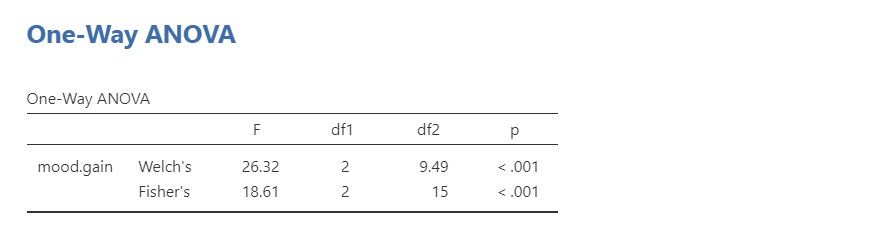
\includegraphics[width=1\linewidth]{images/04_one-way-anova/one-way_results_Welch} 

}

\caption{One-way ANOVA results in jamovi}\label{fig:unnamed-chunk-5}
\end{figure}

\begin{quote}
Using a Welch's F-test, there is a significant difference in mood gain across the three drug conditions, \emph{F} (2, 9.49) = 26.32, \emph{p} \textless{} .001.
\end{quote}

\hypertarget{kruskal-wallis-test}{%
\subsubsection{Kruskal-Wallis test}\label{kruskal-wallis-test}}

To perform the Kruskal-Wallis test in jamovi, you will need to select under the ANOVA button ``One-Way ANOVA, Kruskal Wallis'' towards the bottom of the list of options. Move \texttt{mood.gain} to the Dependent Variables box and \texttt{drug} to the Grouping Variable box. Select Effect size; if you need post hoc comparisons select DSCF pairwise comparisons (see section below on group differences). You will interpret the results similarly to the one-way ANOVA:

\begin{figure}

{\centering 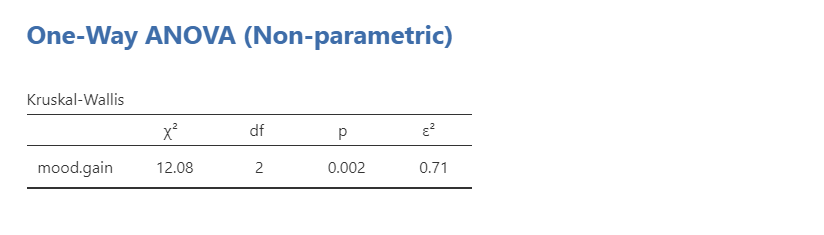
\includegraphics[width=1\linewidth]{images/04_one-way-anova/one-way_results_Kruskal} 

}

\caption{Kruskal-Wallis results in jamovi}\label{fig:unnamed-chunk-6}
\end{figure}

\begin{quote}
Using a Kruskal-Wallis test, there is a significant difference in mood gain across the three drug conditions, \(\chi^2\) (2) = 12.08, \emph{p} = .002, \(\epsilon^2\) = .71.
\end{quote}

Notice how in this case all three results converge and show there is a statistically significant difference in the results! The problem is\ldots{} differences in which groups?

\hypertarget{additional-information-3}{%
\subsection{Additional information}\label{additional-information-3}}

\hypertarget{relationship-between-anova-and-t-test}{%
\subsubsection{Relationship between ANOVA and t-test}\label{relationship-between-anova-and-t-test}}

An ANOVA with two groups is identical to the t-test. That means the F and t statistics are directly related, and you will get the same p-value. For example, imagine you run a t-test and get a t-statistic of \emph{t} (16) = -1.31, \emph{p} = .210. If you ran it as a one-way ANOVA, you would get an F-statistic of \emph{F} (1, 16) = 1.71, \emph{p} = .210.

\(F = t^2\)

\(t = \sqrt{F}\)

Just a fun little bit of trivia! So if you accidentally do an F-test with two groups, no need to go back and redo the analyses (although you should if you are sharing your code for reproducibility). You can just convert your F to a t statistic easily!

\hypertarget{a-note-on-one-tailed-vs.-two-tailed-tests}{%
\subsubsection{A note on one-tailed vs.~two-tailed tests}\label{a-note-on-one-tailed-vs.-two-tailed-tests}}

Unlike a t-test, we would not halve the p-value in an F-ratio because it is an omnibus test. Our planned contrasts or post-hoc tests can tell us where differences are, and we can provide directional hypotheses there if we so choose.

\hypertarget{your-turn-5}{%
\subsection{Your turn!}\label{your-turn-5}}

Open the \texttt{Sample\_Dataset\_2014.xlsx} file that we will be using for all Your Turn exercises. You can find the dataset here: \href{https://github.com/danawanzer/stats-with-jamovi/blob/master/data/Sample_Dataset_2014.xlsx}{Sample\_Dataset\_2014.xlsx Download}

Perform one-way ANOVAs based on the following research questions. Check your assumptions and ensure you are using the correct tests.

To get the most out of these exercises, try to first find out the answer on your own and then use the drop-down menus to check your answer.

\begin{enumerate}
\def\labelenumi{\arabic{enumi}.}
\item
  \textbf{Does students differ on English scores by rank (i.e., freshmen, sophomore, junior, senior)?}

  \begin{itemize}
  \item
    Do you satisfy the assumption of normality? yes no
  \item
    Do you satisfy the assumption of homogeneity of variance? yes no
  \item
    Which statistic should you use? one-way ANOVA Welch's F-test Kruskal-Wallis test
  \item
    Do students differ on English scores by rank? yes no
  \end{itemize}
\item
  \textbf{Does smoking status (Smoking: Nonsmoker = 0, Past smoker = 1, Current smoker = 2) relate to sprint time?}

  \begin{itemize}
  \item
    Do you satisfy the assumption of normality? yes no
  \item
    Do you satisfy the assumption of homogeneity of variance? yes no
  \item
    Which statistic should you use? one-way ANOVA Welch's F-test Kruskal-Wallis test
  \item
    Does smoking status relate to sprint time? yes no
  \end{itemize}
\end{enumerate}

\hypertarget{finding-group-differences}{%
\section{Finding Group Differences}\label{finding-group-differences}}

Often, we're not interested in just \emph{whether} there is a difference (which the F-statistic can tell us), but \emph{where} the differences are between groups (which the F-statistic cannot tell us). For that, we use either \underline{planned contrasts} when you have specific hypotheses you want to test or \underline{post-hoc comparisons} when you have no specific hypotheses.

\textbf{Note}: You \underline{do not} perform contrasts or post hoc comparisons if your overall \(F\) statistic is not statistically significant. You do not interpret group differences if you fail to reject the null hypothesis that there are no group differences!

\hypertarget{planned-contrasts}{%
\subsection{Planned Contrasts}\label{planned-contrasts}}

If you have before-analysis hypotheses of group differences in your data, you will use planned contrasts. You can find the planned contrasts in the ANOVA (but not the one-way ANOVA) setup as a drop-down menu. Note that while I show all six contrasts that jamovi provides, you do not normally do multiple contrasts. These are just shown for illustrative purposes:

\begin{enumerate}
\def\labelenumi{\arabic{enumi}.}
\tightlist
\item
  \textbf{Deviation}: compares the effect of each category (except the first category) to the overall experimental effect. The order of categories is alphabetical or numerical order. Notice how anxifree is considered the first category.
\end{enumerate}

\begin{figure}

{\centering 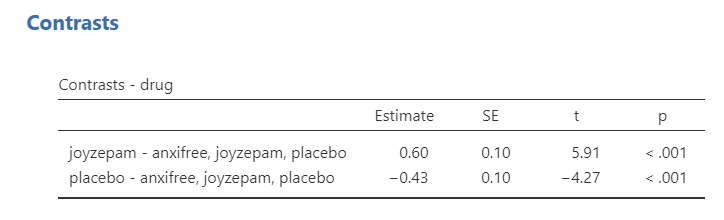
\includegraphics[width=1\linewidth]{images/04_one-way-anova/contrasts_deviation} 

}

\caption{Contrasts - Deviation}\label{fig:unnamed-chunk-1}
\end{figure}

\begin{enumerate}
\def\labelenumi{\arabic{enumi}.}
\setcounter{enumi}{1}
\tightlist
\item
  \textbf{Simple}: Each category is compared to the first category. The order of categories is alphabetical or numerical order. Notice how anxifree is considered the first category.
\end{enumerate}

\begin{figure}

{\centering 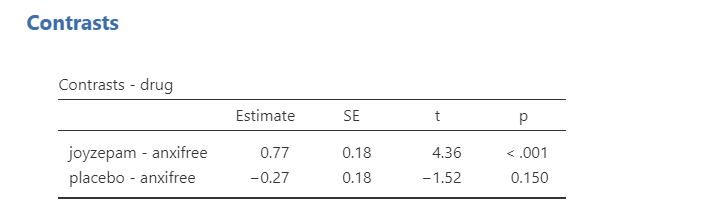
\includegraphics[width=1\linewidth]{images/04_one-way-anova/contrasts_simple} 

}

\caption{Contrasts - Simple}\label{fig:unnamed-chunk-2}
\end{figure}

\begin{enumerate}
\def\labelenumi{\arabic{enumi}.}
\setcounter{enumi}{2}
\tightlist
\item
  \textbf{Difference}: Each category (except the first) is compared to the mean effect of all previous categories.
\end{enumerate}

\begin{figure}

{\centering 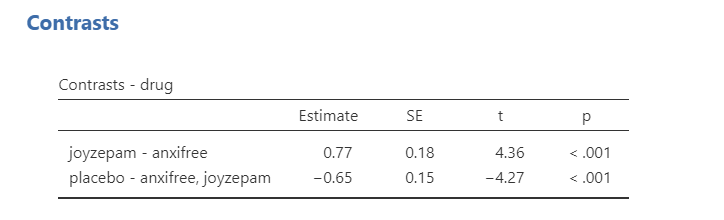
\includegraphics[width=1\linewidth]{images/04_one-way-anova/contrasts_difference} 

}

\caption{Contrasts - Difference}\label{fig:unnamed-chunk-3}
\end{figure}

\begin{enumerate}
\def\labelenumi{\arabic{enumi}.}
\setcounter{enumi}{3}
\tightlist
\item
  \textbf{Helmert}: Each category (except the last) is compared to the mean effect of all subsequent categories.
\end{enumerate}

\begin{figure}

{\centering 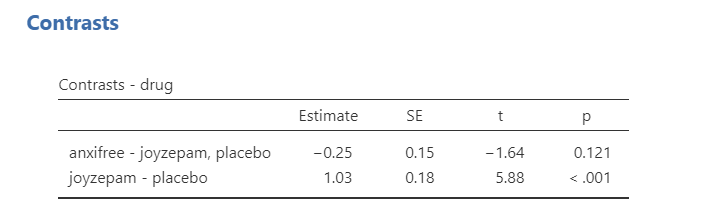
\includegraphics[width=1\linewidth]{images/04_one-way-anova/contrasts_helmert} 

}

\caption{Contrasts - Helmert}\label{fig:unnamed-chunk-4}
\end{figure}

\begin{enumerate}
\def\labelenumi{\arabic{enumi}.}
\setcounter{enumi}{4}
\tightlist
\item
  \textbf{Repeated}: Each category is compared to the last category.
\end{enumerate}

\begin{figure}

{\centering 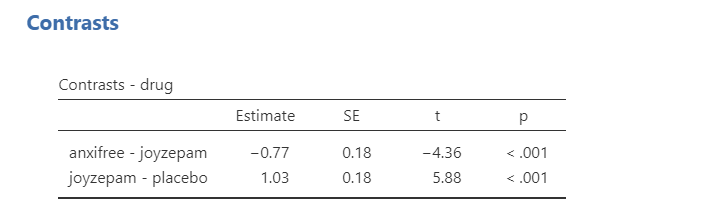
\includegraphics[width=1\linewidth]{images/04_one-way-anova/contrasts_repeated} 

}

\caption{Contrasts - Repeated}\label{fig:unnamed-chunk-5}
\end{figure}

\begin{enumerate}
\def\labelenumi{\arabic{enumi}.}
\setcounter{enumi}{5}
\tightlist
\item
  \textbf{Polynomial}: Tests trends in the data. It will examine the \emph{n-1}\textsuperscript{th} degree based on the number of groups. In this case, because we have 3 groups it is testing both a linear (\textsuperscript{1}) and quadratic (\textsuperscript{2}) trend. If we had 5 groups, it would test a linear (\textsuperscript{1}), quadratic (\textsuperscript{2}), cubic (\textsuperscript{3}), and quartic (\textsuperscript{4}) trend. Note that your factor levels must be ordinal for a polynomial contrast to make sense.
\end{enumerate}

\begin{figure}

{\centering 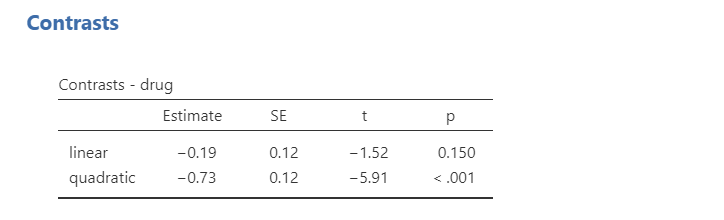
\includegraphics[width=1\linewidth]{images/04_one-way-anova/contrasts_polynomial} 

}

\caption{Contrasts - Polynomial}\label{fig:unnamed-chunk-6}
\end{figure}

\textbf{Test yourself!} Which contrast would make \underline{most sense} to test given that we want to know how our drug compares to the other two drugs? deviation simple difference helmert repeated polynomial

\hypertarget{write-up-planned-contrasts-in-apa-style}{%
\subsubsection{Write up planned contrasts in APA style}\label{write-up-planned-contrasts-in-apa-style}}

Here's some example write-ups of the above results.

\begin{quote}
There is a significant difference in mood gain across the three drug conditions, \emph{F} (2, 15) = 18.61, \emph{p} \textless{} .001. Repeated contrasts showed that \emph{Joyzepam} (\emph{M} = 1.48, \emph{SD} = .21) outperformed both \emph{Anxifree} (\emph{M} = .72, \emph{SD} = .39; \emph{p} \textless{} .001) and the placebo condition (\emph{M} = .45, \emph{SD} = .28; \emph{p} \textless{} .001).

(Note how this example makes no sense because our data is not ordinal) There is a significant difference in mood gain across the three drug conditions, \emph{F} (2, 15) = 18.61, \emph{p} \textless{} .001. There was not a significant linear trend across the drug conditions (\emph{p} = .150).
\end{quote}

\hypertarget{post-hoc-comparisons}{%
\subsection{Post hoc comparisons}\label{post-hoc-comparisons}}

Often, we do not have any \emph{a priori} (or planned) predictions or hypotheses about our group differences. In this case, we use post hoc procedures. These procedures do \underline{pairwise comparisons} among all of our groups, like t-tests across each of our groups. As we noted on the first page of this handout, this can be highly problematic for our Type I error rate! Therefore, we must perform corrections to control our familywise error rate.

jamovi currently supports five types of post-hoc tests; I generally only use Tukey or Bonferonni:

\begin{enumerate}
\def\labelenumi{\arabic{enumi}.}
\tightlist
\item
  \textbf{No correction}: This doesn't correct for a Type I error at all. Don't use this! I won't even show it. It's bad. Never use it. NEVER. You are warned!
\item
  \textbf{Tukey}: This is the post hoc test I use most often. It controls the Type I error rate well, but isn't as conservative of a control as the Bonferonni.
\item
  \textbf{Scheffe}: Honestly, I've never used it. I am not sure how it's calculated.
\item
  \textbf{Bonferroni}: This is the most conservative test. It's good if you only have a small number of comparisons to make or if you \emph{really} want to control your Type I error rate. If you have a lot of them to test , then you should use something else.
\item
  \textbf{Holm}: Honestly, I've never used it. I am not sure how it's calculated.
\end{enumerate}

Games-Howell for when you have unequal variances and Tukey for when you have equal variances. They will each calculate your p-values slightly differently but in a way to control for our Type I error rate as best it can. They are interpreted very similarly, so we will proceed with the Tukey's post hoc comparisons because we satisfied the assumption of equal variances.

To request post hoc tests from the one-way ANOVA, open the collapsed menu at the bottom of the setup menu. Select \texttt{Tukey\ (equal\ variances} under Post-Hoc Test and select \texttt{Mean\ difference}, \texttt{Report\ significance}, and \texttt{Flag\ significant\ comparisons} under Statistics. Optionally, you can request the \texttt{Test\ results\ (t\ and\ df)} although this is not necessary.

Below shows the post hoc test results for our one-way ANOVA. Notice the differences in p-values across the four post hoc tests and how all other values are the same. Notice how the Bonferroni is most conservative (i.e., has the largest p-values) and the Holm's is the least conservative (i.e., has the smallest p-values). Keep in mind you do not normally ask for multiple post hoc comparisons. Just pick one! Normally, I just pick Tukey's.

\begin{figure}

{\centering 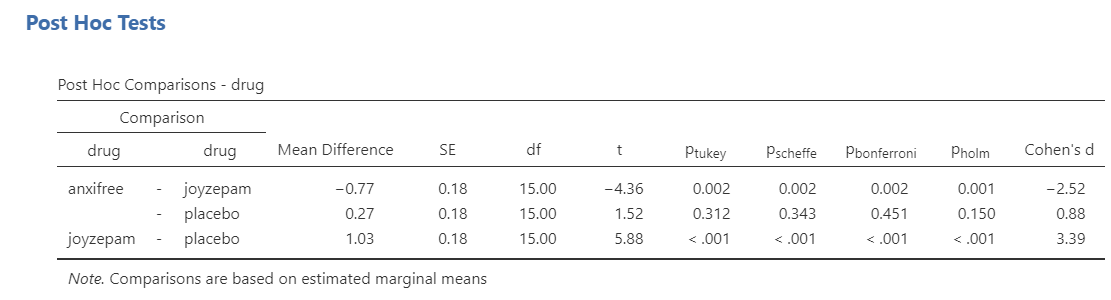
\includegraphics[width=1\linewidth]{images/04_one-way-anova/one-way_results_post-hoc} 

}

\caption{Post hoc test results in jamovi}\label{fig:unnamed-chunk-7}
\end{figure}

\hypertarget{write-up-post-hoc-results-in-apa-style}{%
\subsubsection{Write up post hoc results in APA style}\label{write-up-post-hoc-results-in-apa-style}}

The way we would write up each of the post hoc comparisons is very similar. Given that I usually use Tukey, here is a write-up for those results:

\begin{quote}
There is a significant difference in mood gain across the three drug conditions, \emph{F} (2, 15) = 18.61, \emph{p} \textless{} .001. Post hoc comparisons using Tukey's HSD revealed that our drug \emph{Joyzepam} (\emph{M} = 1.48, \emph{SD} = .21) outperformed both \emph{Anxifree} (\emph{M} = .72, \emph{SD} = .39; \emph{p} = .002) and the placebo condition (\emph{M} = .45, \emph{SD} = .28; \emph{p} \textless{} .001); there were no differences between \emph{Anxifree} and the placebo condition (\emph{p} = .312).
\end{quote}

Writing up results in APA style is both a science and an art. There's a science to what you need to report. For example, you always report the statistics exactly the same: \emph{F} (df\textsubscript{WG}, df\textsubscript{BG}) = X.XX, \emph{p} = .XXX. You also always report the group means (\emph{M}) and standard deviations (\emph{SD}), although you can report them in-text like I did above or in a descriptives table like you can ask from jamovi.

However, there's also an art to it. Notice how I wrote that up in a way to summarize the findings as succinctly as possible. I could have said there was a difference between \emph{anxifree} and \emph{joyzepam} and a difference between \emph{joyzepam} and the placebo, but that's a lot more words and isn't written in a way to focus on what I'm hoping to see: that my drug \emph{joyzepam} performed better than the competitor \emph{anxifree} and a placebo condition.

This is where you need to think creatively and be very critical in checking that what you say makes sense. Read your write-ups carefully! Have someone else read it. Can they understand what you mean?

\hypertarget{in-case-of-violated-assumptions-5}{%
\subsection{In case of violated assumptions}\label{in-case-of-violated-assumptions-5}}

If you are using Welch's F-test using the One-Way ANOVA in jamovi, you should select under Post-Hoc Tests \texttt{Games-Howell\ (unequal\ variances)}. These will be interpreted similarly to the post hoc comparisons above.

If you are using the Kruskal-Wallis test, you will select the check-box for \texttt{DSCF\ pairwise\ comparisons}. This stands for the Dwass-Steel-Critchlow-Fligner test. All you need to know is that they, too, are interpreted similarly to the post hoc comparisons above.

Unfortunately, you cannot perform contrasts with either the Welch's F-test or Kruskal-Wallis test.

\hypertarget{your-turn-6}{%
\subsection{Your turn!}\label{your-turn-6}}

Open the \texttt{Sample\_Dataset\_2014.xlsx} file that we will be using for all Your Turn exercises. You can find the dataset here: \href{https://github.com/danawanzer/stats-with-jamovi/blob/master/data/Sample_Dataset_2014.xlsx}{Sample\_Dataset\_2014.xlsx Download}

Perform one-way ANOVAs based on the following research questions. Check your assumptions and ensure you are using the correct tests.

To get the most out of these exercises, try to first find out the answer on your own and then use the drop-down menus to check your answer.

\textbf{Note}: These are the same questions as in the one-way ANOVA chapter, but now you focus on the group differences.

\begin{enumerate}
\def\labelenumi{\arabic{enumi}.}
\item
  \textbf{Does students differ on English scores by rank (i.e., freshmen, sophomore, junior, senior)?}

  \begin{itemize}
  \item
    Should you perform a planned contrast or post hoc comparison? planned contrast post hoc
  \item
    What are the results of the post hoc comparison? N/A - Don't perform Freshmen had higher English scores than sophomores, juniors, and seniors Freshmen and sophomores had higher English scores than juniors and seniors
  \end{itemize}
\item
  \textbf{Does smoking status (Smoking: Nonsmoker = 0, Past smoker = 1, Current smoker = 2) relate to sprint time?}

  \begin{itemize}
  \item
    Should you perform a planned contrast or post hoc comparison? planned contrast post hoc
  \item
    What are the results of the post hoc comparison? N/A - Don't perform Nonsmokers had significantly faster sprint times than current smokers Nonsmokers and past smokers had significantly faster spring times than current smokers Nonsmokers had significantly faster sprint times than both past and current smokers
  \end{itemize}
\end{enumerate}

\hypertarget{repeated-measures-anova}{%
\section{Repeated Measures ANOVA}\label{repeated-measures-anova}}

\hypertarget{overview-7}{%
\subsection{Overview}\label{overview-7}}

The repeated measures analysis of variance (ANOVA) is used to test the difference in our dependent variable between \underline{three or more} groups of observations in which all participants participate in all groups or levels. Our grouping variable is our independent variable. In other words, we use the one-way ANOVA when we have a research question with a \textbf{continuous dependent variable} and a \textbf{categorical independent variable with three or more categories in which the same participants are in each category}.

The repeated measures ANOVA is also sometimes called the one-way related ANOVA.

There are two ways we could have the repeated measures ANOVA. Perhaps the same group of participants are measured in the same dependent variable at three or more time points. In this case, our independent variable is time and our dependent variable is whatever is measured at each time point.

\begin{figure}

{\centering \includegraphics[width=0.8\linewidth]{images/05-repeated-measures-anova/Laerd1} 

}

\caption{Repeated measures ANOVA by Time}\label{fig:unnamed-chunk-1}
\end{figure}

The other way we might have the repeated measures ANOVA is if all our participants participate in all conditions of our study. In this case, our independent variable is the treatment or condition and the dependent variable is whatever is measured in each treatment or condition.

\begin{figure}

{\centering \includegraphics[width=0.8\linewidth]{images/05-repeated-measures-anova/Laerd2} 

}

\caption{Repeated measures ANOVA by Conditions}\label{fig:unnamed-chunk-2}
\end{figure}

\hypertarget{look-at-the-data-7}{%
\subsection{Look at the data}\label{look-at-the-data-7}}

Let's run an example with data from lsj-data. Open data from your Data Library in ``lsj-data''. Select and open ``broca''.

This dataset is hypothetical data in which six patients suffering from Broca's Aphasia (a language deficit commonly experienced following a stroke) complete three word recognition tasks. On the first (speech production) task, patients were required to repeat single words read out aloud by the researcher. On the second (conceptual) task, designed to test word comprehension, patients were required to match a series of pictures with their correct name. On the third (syntax) task, designed to test knowledge of correct word order, patients were asked to reorder syntactically incorrect sentences. Each patient completed all three tasks. The order in which patients attempted the tasks was counterbalanced between participants. Each task consisted of a series of 10 attempts. The number of attempts successfully completed by each patient are provided in the dataset.

\hypertarget{data-set-up-7}{%
\subsubsection{Data set-up}\label{data-set-up-7}}

To conduct the repeated measures ANOVA, we first need to ensure our data is set-up properly in our dataset. This requires having two columns: one with our continuous dependent variable and one indicating which group the participant is in. Each row is a unique participant or unit of analysis.

INCLUDE DATA SETUP HERE

In the data above, what is your \textbf{independent variable}? ID Semester TestScore

In the data above, what is your \textbf{dependent variable}? ID Semester TestScore

\hypertarget{describe-the-data-6}{%
\subsubsection{Describe the data}\label{describe-the-data-6}}

\hypertarget{check-assumptions-5}{%
\subsection{Check Assumptions}\label{check-assumptions-5}}

\hypertarget{assumptions-4}{%
\subsubsection{Assumptions}\label{assumptions-4}}

As a parametric test, the repeated measures ANOVA has the same assumptions as other parametric tests:

\begin{enumerate}
\def\labelenumi{\arabic{enumi}.}
\item
  The dependent variable is \textbf{normally distributed}
\item
  Variances in the two groups are roughly equal (i.e., \textbf{homogeneity of variances}); in repeated measures ANOVA this is called the assumption of \textbf{sphericity}
\item
  The dependent variable is \textbf{interval or ratio} (i.e., continuous)
\item
  \sout{Scores are \textbf{independent} between groups} (this assumption is not relevant because all participants participate in all conditions)
\end{enumerate}

We cannot \emph{test} the third and fourth assumptions; rather, those are based on knowing your data.

However, we can and should test for the first two assumptions. Fortunately, the one-way ANOVA in jamovi has three check boxes under ``Assumption Checks'' that lets us test for both assumptions.

\hypertarget{sphericity-assumption}{%
\paragraph{Sphericity Assumption}\label{sphericity-assumption}}

The sphericity assumption is essentially the repeated measures ANOVA equivalent of homogeneity of variances. Sphericity means there is equality of variances of the \emph{differences} between treatment levels. For example, if there are three groups, then the difference in all three pairs of differences (1-2, 1-3, 2-3) need to have approximately equal variances. You only need to care about sphericity when there are at least three conditions, which is why we did not talk about this with the dependent t-test.

Fortunately, like the other assumption checks, testing for sphericity is as simple as a checkbox in jamovi.

\hypertarget{checking-assumptions-4}{%
\subsubsection{Checking assumptions}\label{checking-assumptions-4}}

You'll notice there are no options to check for normality in the repeated measures ANOVA in jamovi. There's an \href{https://forum.jamovi.org/viewtopic.php?f=5\&t=1045}{interesting conversation} on the topic in the jamovi forums. Suffice to say, it's complicated and maybe someday they will implement it. For now, we just won't worry about it for the repeated measures ANOVA.

So what we need to worry about is testing our assumption of sphericity. You should have checked the box \texttt{Sphericity\ tests} under the Assumption Checks drop-down menu. That produces the following output:

\begin{figure}

{\centering \includegraphics[width=1\linewidth]{images/05-repeated-measures-anova/rm-anova_sphericity} 

}

\caption{Testing sphericity in jamovi}\label{fig:unnamed-chunk-3}
\end{figure}

Mauchly's test of sphericity tests the null hypothesis that the variances of the differences between the conditions are equal. Therefore, just like with our previous assumption checks, if Mauchly's test is non-significant (i.e., \emph{p} \textgreater{} .05, as is the case in this analysis) then it is reasonable to conclude that the variances of the differences are not significantly different. This means we satisfy the assumption of sphericity and can conclude that the variances of the differences are roughly equal.

If Mauchly's test had been statistically significant (\emph{p} \textless{} .05), then we would conclude that the assumption had \emph{not} been met. In this case, we should apply a correction to the \emph{F}-value obtained in the repeated measures ANOVA:

\begin{itemize}
\tightlist
\item
  If the Greenhouse-Geisser value in the ``Tests of Sphericity'' table is \textgreater{} .75 then you should use the Huynh-Feldt correction.
\item
  If the Greenhouse-Geisser value is \textless{} .75, then you should use the Greenhouse-Geisser correction.
\end{itemize}

You can select these corrections in the Assumption Checks drop-down menu.

\hypertarget{perform-the-test-7}{%
\subsection{Perform the test}\label{perform-the-test-7}}

\begin{enumerate}
\def\labelenumi{\arabic{enumi}.}
\item
  To perform a repeated measures ANOVA in jamovi, go to the Analyses tab, click the ANOVA button, and choose ``Repeated Measures ANOVA''.
\item
  Under ``Repeated Measures Factors'' name your independent variable. In this case you can name it ``Task''. Rename the three levels of Task: Speech, Conceptual, and Syntax.
\item
  Under ``Repeated Measures Cells'' move the given variable into the correct level. For example, you'll move Speech to the Speech cell.
\item
  Select Generalised \(\eta^2\) as your measure of effect size.
\item
  In the Assumption Checks drop-down menu, select \texttt{Sphericity\ tests}. You'll note that if you violate the assumption of sphericity, there are two corrections provided. These will be discussed later.
\item
  In the Post Hoc Tests drop-down menu, select \texttt{Tukey}. Remember that we only interpret these if the overall \emph{F} is statistically significant.
\item
  In the Estimated Marginal Means drop-down menu, move Task to the Marginal Means box, select \texttt{Marginal\ means\ tables}, and select \texttt{Observed\ scores} . Uncheck \texttt{Equal\ cell\ weights}.
\end{enumerate}

When you are done, your setup should look like this:

\begin{figure}

{\centering \includegraphics[width=0.8\linewidth]{images/05-repeated-measures-anova/rm-anova_setup1} 

}

\caption{Repeated Measures ANOVA setup in jamovi}\label{fig:unnamed-chunk-4}
\end{figure}

\begin{figure}

{\centering \includegraphics[width=0.8\linewidth]{images/05-repeated-measures-anova/rm-anova_setup2} 

}

\caption{Repeated Measures ANOVA setup in jamovi}\label{fig:unnamed-chunk-5}
\end{figure}

\hypertarget{interpret-results-5}{%
\subsection{Interpret results}\label{interpret-results-5}}

Once we are satisfied we have satisfied the assumptions for the repeated measures, we can interpret our results.

\begin{figure}

{\centering \includegraphics[width=1\linewidth]{images/05-repeated-measures-anova/rm-anova_results} 

}

\caption{One-way ANOVA results in jamovi}\label{fig:unnamed-chunk-6}
\end{figure}

You'll notice that jamovi provides you both a Within Subjects Effects table and Between Subjects Effects table. However, we only have a within-subjects effect (Task). Why did it give us a between-subjects table? With the repeated-measures ANOVA (which only has within-subjects IVs), this is just our \(SS_{BG}\). However, because we don't have one, it's not calculating anything. We can ignore it. It is only useful if we are conducting a mixed factorial ANOVA with both between-subjects and within-subjects effects.

Therefore, the Within Subjects Effects table is of most use to us. We can see that the overall effect of Task is statistically significant (\emph{p} = .013). Therefore we can look at our Post Hoc Tests results.

\begin{figure}

{\centering \includegraphics[width=1\linewidth]{images/05-repeated-measures-anova/rm-anova_tukey} 

}

\caption{One-way ANOVA results in jamovi}\label{fig:unnamed-chunk-7}
\end{figure}

The Tukey post hoc differences show that there was a significant difference between speech and syntax (\emph{p} = .011), but not between conceptual and both speech and syntax. Last, we can look at the Estimated Marginal Means - Task table to see the group means for reporting purposes. This shows us that participants recognized significantly more words in the speech task than in the syntax task.

\hypertarget{write-up-the-results-in-apa-style-7}{%
\subsubsection{Write up the results in APA style}\label{write-up-the-results-in-apa-style-7}}

We can write this up in APA style similar to the one-way ANOVA.

\begin{quote}
A repeated measures ANOVA was performed examining how three tasks affected word recognition in patients suffering from Broca's Aphasia. Task significantly affected word recall, \emph{F} (2, 10) = 6.93, \emph{p} = .013, \(\eta^2_G\) = .41. Tukey's post hoc difference tests indicated that participants recognized significantly more words in the speech task (\emph{M} = 7.17, \emph{SE} = .62) than participants in the syntax task (\emph{M} = 4.33, \emph{SE} = .62; \emph{p}~= .011). There were no differences between the conceptual task (\emph{M} = 6.17, \emph{SE} = .62) and both the speech and syntax tasks.
\end{quote}

\hypertarget{visualize-the-results-7}{%
\subsubsection{Visualize the results}\label{visualize-the-results-7}}

\hypertarget{in-case-of-violated-assumptions-6}{%
\subsection{In case of violated assumptions}\label{in-case-of-violated-assumptions-6}}

We have already discussed what to do if you violate the assumption of sphericity above; you select one of the two sphericity corrections.

If you violate the assumption of normality or if the dependent variable is ordinal, then you can use the Friedman test. You can select this using the Repeated Measures ANOVA - Friedman option under the ANOVA analysis.

\hypertarget{friedmans-test}{%
\subsubsection{Friedman's test}\label{friedmans-test}}

Friedman's test can only examine one within-subjects variable, so you will move all three conditions (Speech, Conceptual, and Syntax) to the Measures box. Select \texttt{Pairwise\ comparisons\ (Durbin-Conover} for post hoc comparisons and \texttt{Descriptives} for the Means and Medians. Optionally, you can select to plot either the Means or Medians. The Setup is shown below.

\begin{figure}

{\centering \includegraphics[width=0.8\linewidth]{images/05-repeated-measures-anova/rm-anova_friedman_setup} 

}

\caption{Repeated Measures ANOVA setup in jamovi}\label{fig:unnamed-chunk-8}
\end{figure}

Once you've set-up the analysis, you can interpret the results. Overall, we continue to see a statistically significant result and that there is only a significant difference between speech and syntax.

\begin{figure}

{\centering \includegraphics[width=1\linewidth]{images/05-repeated-measures-anova/rm-anova_friedman} 

}

\caption{Repeated Measures ANOVA setup in jamovi}\label{fig:unnamed-chunk-9}
\end{figure}

We can write up the results similarly as before:

\begin{quote}
Friedman's test was performed examining how three tasks affected word recognition in patients suffering from Broca's Aphasia. Task significantly affected word recall, \(\chi^2\) (2) = 6.64, \emph{p} = .036. Pairwise comparisons using Durbin-Conover indicated that participants recognized significantly more words in the speech task (\emph{M} = 7.17, \emph{Mdn} = 7.50) than participants in the syntax task (\emph{M} = 4.33, \emph{Mdn} = 6.50; \emph{p} = .006). There were no differences between the conceptual task (\emph{M} = 6.17, \emph{Mdn} = 6.50) and both the speech and syntax tasks.
\end{quote}

\hypertarget{your-turn-7}{%
\subsection{Your turn!}\label{your-turn-7}}

Open the \texttt{Sample\_Dataset\_2014.xlsx} file that we will be using for all Your Turn exercises. You can find the dataset here: \href{https://github.com/danawanzer/stats-with-jamovi/blob/master/data/Sample_Dataset_2014.xlsx}{Sample\_Dataset\_2014.xlsx Download}

Perform a repeated measures ANOVA based on the following research questions. Check your assumptions and ensure you are using the correct tests.

To get the most out of these exercises, try to first find out the answer on your own and then use the drop-down menus to check your answer.

\begin{enumerate}
\def\labelenumi{\arabic{enumi}.}
\item
  \textbf{Does students differ on their test scores (English, Reading, Math, Writing)?}

  \begin{itemize}
  \item
    Based on your understanding of the nature of the test scores, which statistic should you use? repeated measures ANOVA Friedman's test
  \item
    Should you apply a sphericity correction? If so, which one? N/A - using Friedman's test no, assumption satisfed yes, Greenhouse-Geisser yes, Huynh-Feldt
  \item
    Do students differ on their test scores? yes no
  \item
    Should you perform a planned contrast or post hoc comparison? yes no
  \item
    What are the results of the post hoc comparison? N/A - Don't perform All test scores were significantly different from one another All test scores were significantly different from one another except for English and Reading
  \end{itemize}
\end{enumerate}

\hypertarget{factorial-anova}{%
\section{Factorial ANOVA}\label{factorial-anova}}

\hypertarget{overview-8}{%
\subsection{Overview}\label{overview-8}}

Factorial ANOVA allows us to examine two or more independent variables (IVs) simultaneously. There are several types of factorial designs:

\begin{itemize}
\tightlist
\item
  \textbf{Independent factorial design}: several between-group (independent) IVs
\item
  \textbf{Repeated measures factorial design}: several within-group (repeated-measures) IVs
\item
  \textbf{Mixed factorial design}: some between-group and some within-group IVs
\end{itemize}

Furthermore, you may read about ANOVAs referred to as ``one-way'', ``two-way'', ``three-way'' or greater. This simply refers to how many independent variables there are. Factorial ANOVAs are sometimes also referenced by how many groups per IV there are; for example, a 2 x 3 ANOVA is a factorial ANOVA in which the first IV has two conditions and the second IV has three conditions. You would also specify which IVs are between-group and which are within-group. For example, you might write that your design is a 2 (between-subjects: gender) x3 (within-subjects: task) mixed factorial.

We won't be going into too much detail on the different factorial ANOVA designs. Instead, I will walk through illustrative cases so that if you want to apply them in the future you can mimic the procedures below.

\hypertarget{independent-factorial-anova}{%
\subsection{Independent Factorial ANOVA}\label{independent-factorial-anova}}

The independent factorial ANOVA has multiple between-group IVs. Let's run an example with data from lsj-data. Open data from your Data Library in ``lsj-data''. Select and open ``rtfm''. This data has two IVs: attend (whether or not the student turned up to lectures) and reading (whether or not the student actually read the textbook). 1 = they did and 0 = they did not.

Because we do not have a within-group IV, we will select the ANOVA analysis. Move grade to your Dependent Variable box and both attend and reading to your Fixed Factors. Select all the same options as you did for the one-way ANOVA (i.e., \(\omega^2\), assumption checks, Tukey's post hoc tests for the two variables attend and reading, estimated marginal means).

Let's go through the output (check that your output matches!) and then discuss how to write up the results in APA format. First, we need to check assumptions. The Levene's test and Shapiro-Wilk's test are shown below. We can see that we meet the assumption of normality but fail to meet the assumption of homogeneity of variance. Unfortunately, we cannot perform a Welch's F-test with more than one independent factorial so we will note this failed assumption and move on.

\begin{figure}

{\centering \includegraphics[width=1\linewidth]{images/06-factorial-anova/independent-factorial_assumptions} 

}

\caption{Assumption check results in jamovi}\label{fig:unnamed-chunk-1}
\end{figure}

Let's look at the main results next. We got three lines of results in addition to the typical residuals (error). The first two lines are our main effects of \texttt{attend} and \texttt{reading} on grades. The p-values for both are statistically significant indicating attend affects grades and reading affects grades. However, it also added an interaction term of \texttt{attend\ *\ reading}, which is not statistically significant. This means we do not have an interaction between attend and reading on grades. Interactions will be discussed in more detail in the next section.

\begin{figure}

{\centering \includegraphics[width=1\linewidth]{images/06-factorial-anova/independent-factorial_results} 

}

\caption{Independent factorial ANOVA results in jamovi}\label{fig:unnamed-chunk-2}
\end{figure}

Although we could simply look at the means to know whether attending or reading had higher grades than not attending or not reading because there are only two conditions, we can also look at the post hoc tests and definitely need to look at them if we have three or more conditions per IV. These are shown below. Because the mean differences are negative, we can determine that the second group had higher means than the second group. We can confirm that with the estimated marginal means (not shown here).

\begin{figure}

{\centering \includegraphics[width=1\linewidth]{images/06-factorial-anova/independent-factorial_posthoc} 

}

\caption{Post hoc results in jamovi}\label{fig:unnamed-chunk-3}
\end{figure}

Last, we can write-up our results!

\begin{quote}
We were interested in knowing how attendance and reading affected student grades. An independent factorial ANOVA showed that both attendance (\emph{F} {[}1, 4{]} = 18.25, \emph{p} = .013, \(\omega^2\) = .26) and reading (\emph{F} {[}1, 4{]} = 44.17, \emph{p} = .003, \(\omega^2\) = .64) affected student grades; there was no significant interaction between attendance and reading (\emph{F} {[}1, 4{]} = 8.00, \emph{p} = .660, \(\omega^2\) = -.01). Post hoc comparisons using Tukey's HSD show that students who attended lectures (\emph{M} = 75.50, \emph{SE} = 2.98) had higher grades than students who did not (\emph{M}~= 57.50, \emph{SE} = 2.98; \emph{p} = .003, \emph{d} = 4.70); furthermore, students who read (\emph{M} = 80.50, \emph{SE} = 2.98) had higher grades than students who did not (\emph{M} = 52.50, \emph{SE} = 2.98; \emph{p} = .013; \emph{d} = 3.02).
\end{quote}

\hypertarget{interactions}{%
\subsubsection{Interactions}\label{interactions}}

Interactions occur when the effect of one IV on the DV depends on the lvel of the other IV. If you did not want to test for interaction effects, you could remove them from the Model Terms in the Model drop-down menu.

However, by default they will include them. If you have 2-3 IVs, it may be reasonable to look at these interactions. However, 3-variable interactions (e.g., IV1 * IV2 * IV3) are pushing it and 4-variable interactions are highly implausible. Be critical in which interaction terms you include!

jamovi can provide a plot of your interaction, which can be helpful to help interpret your results. Below is the plot for our interaction of attendance on reading.

\begin{figure}

{\centering \includegraphics[width=1\linewidth]{images/06-factorial-anova/independent-factorial_plot} 

}

\caption{Interaction plot in jamovi}\label{fig:unnamed-chunk-4}
\end{figure}

The parallel lines that are sloping upward tell me there is a significant main effect for both IVs but no interaction. How do I know that? With two variables, there are only so many interaction shapes possible. \href{https://courses.washington.edu/smartpsy/interactions.htm}{This website} does a fantastic time showing you all 8 combinations of the three effects (2 main effects and 1 interaction effect). Spend some time looking through it and familiarizing yourself with the plots!

\hypertarget{repeated-measures-factorial-anova}{%
\subsection{Repeated Measures Factorial ANOVA}\label{repeated-measures-factorial-anova}}

This is also sometimes called the two-way (or three-way or n-way, depending on the \emph{n} of IVs you have) repeated measures ANOVA. Let's go through an example repeated measures factorial ANOVA. The dataset is courtesy of \href{https://www.real-statistics.com/anova-repeated-measures/two-within-subjects-factors/}{Real Statistics Using Excel}.

\begin{quote}
A company has created a new training program for their customer service staff. To test the effectiveness of the program they took a sample of 10 employees and assessed their performance in three areas: ~Product (knowledge of the company's products and services), Client (their ability to relate to the customer with politeness and empathy) and Action (their ability to take action to help the customer). They then had the same 10 employees take the training course and rated their performance after the program in the same three areas. -\href{A\%20company\%20has\%20created\%20a\%20new\%20training\%20program\%20for\%20their\%20customer\%20service\%20staff.\%20To\%20test\%20the\%20effectiveness\%20of\%20the\%20program\%20they\%20took\%20a\%20sample\%20of\%2010\%20employees\%20and\%20assessed\%20their\%20performance\%20in\%20three\%20areas:\%20Product\%20(knowledge\%20of\%20the\%20company’s\%20products\%20and\%20services),\%20Client\%20(their\%20ability\%20to\%20relate\%20to\%20the\%20customer\%20with\%20politeness\%20and\%20empathy)\%20and\%20Action\%20(their\%20ability\%20to\%20take\%20action\%20to\%20help\%20the\%20customer).\%20They\%20then\%20had\%20the\%20same\%2010\%20employees\%20take\%20the\%20training\%20course\%20and\%20rated\%20their\%20performance\%20after\%20the\%20program\%20in\%20the\%20same\%20three\%20areas.\%20Based\%20on\%20the\%20data\%20in\%20Figure\%201,\%20determine\%20whether\%20the\%20program\%20was\%20effective.}{Real Statistics Using Excel}
\end{quote}

You can find the dataset here to follow along: \href{https://github.com/danawanzer/stats-with-jamovi/blob/master/data/Repeated-measures-factorial-ANOVA.xlsx}{Repeated-measures-factorial-ANOVA.xlsx Download}

In jamovi, select Repeated Measures ANOVA under the ANOVA analysis option. Here are the general steps:

\begin{enumerate}
\def\labelenumi{\arabic{enumi}.}
\item
  In Repeated Measures Factors, you'll need to name both factors. Rename \texttt{RM\ Factor\ 1} to Time and \texttt{RM\ Factor\ 2} to Area. Under Time, specify two levels: Pre and Post. Under Area, specify three levels: Product, Client, and Action.
\item
  In Repeated Measures Cells, you'll now have six cells with the combinations of the 6 columns you have. Drag the variable from the left into the correct cell on the right. Be careful here! For example, you need to put the Pre-Product variable into the cell ``Pre, Product''.
\item
  Name your dependent variable label ``Performance'' and select `Generalised \(\eta^2\).
\item
  Under Assumption Checks, select Sphericity tests
\item
  Under Post Hoc Tests, move Area and Time over and select Tukey.
\item
  Under Estimated Marginal Means, move Time over into Term 1, Area into Term 2, and both Time and Area into Term 3. Select plots and tables, Observed scores, and Equal cell weights.
\end{enumerate}

Now let's go over selected output. First, we need to check our assumption of sphericity. All the Mauchly's W's are not statistically significant so we satisfy the assumption of sphericity and do not need to apply any sphericity corrections.

\begin{figure}

{\centering \includegraphics[width=1\linewidth]{images/06-factorial-anova/rm-factorial_assumption} 

}

\caption{Assumption testing in jamovi}\label{fig:unnamed-chunk-5}
\end{figure}

Next let's look at the within subjects effects table. Remember, we do not need to worry about the between subjects effects table because we do not have one; it will be used in the mixed factorial design below. Overall, we see a significant main effect of area, a significant main effect of time, and a significant interaction effect of both area and time. Neat!

\begin{figure}

{\centering \includegraphics[width=1\linewidth]{images/06-factorial-anova/rm-factorial_results} 

}

\caption{Repeated measures ANOVA in jamovi}\label{fig:unnamed-chunk-6}
\end{figure}

Next, we can look at post hoc comparisons because the main effects were all statistically significant. For area, we can see that client and action had significantly higher means than product, but there was no difference between client and action. Furthermore, post-intervention performance was significantly higher than pre-intervention.

\begin{figure}

{\centering \includegraphics[width=1\linewidth]{images/06-factorial-anova/rm-factorial_tukey} 

}

\caption{Post hoc tests in jamovi}\label{fig:unnamed-chunk-7}
\end{figure}

Last, let's look at the interaction to get a sense of what the interaction looks like. It appears that although there are no differences between pre- and post-intervention for product, there are significant differences from pre- to post-intervention for both client and action. To be more specific on where the statistically significant differences are, you can also ask for post hoc tests for the interaction term. This is where including a plot can be very helpful for your audience!

\begin{figure}

{\centering \includegraphics[width=1\linewidth]{images/06-factorial-anova/rm-factorial_interaction} 

}

\caption{Interaction plot in jamovi}\label{fig:unnamed-chunk-8}
\end{figure}

Now we have everything we need (in addition to the estimated marginal means) and can write-up our results.

\begin{quote}
We tested a 2 (time: pre- and post-intervention) x 3 (area: product, client, action) repeated measures factorial design to examine how both time and area affected performance. We satisfied the assumption of sphericity for all effects. There was a significant main effect of time (\emph{F} {[}1, 9{]} = 33.85, \emph{p} \textless{} .001, \(\eta^2_G\) = .25) such that performance at post-intervention (\emph{M} = 26.80, \emph{SE} = 1.84) was higher than at pre-intervention (\emph{M} = 19.37, \emph{SE} = 1.84). There was also a significant main effect of area (\emph{F} {[}2, 18{]} = 26.96, \emph{p} \textless{} .001, \(\eta^2_G\) = .36) such that both client (\emph{M} = 25.10, \emph{SE} = 1.95) and action (\emph{M} = 27.65, \emph{SE}~= 19.5) performance was higher than product performance (\emph{M} = 16.50, \emph{SE} = 1.95), but there was no difference between client and action performance. Lastly, there was a significant interaction between time and area such that there were no differences in product performance from pre- to post-intervention but there was for client and action performance (see Figure 1).
\end{quote}

\hypertarget{mixed-factorial-anova}{%
\subsection{Mixed Factorial ANOVA}\label{mixed-factorial-anova}}

You can find the dataset here to follow along: \href{https://github.com/danawanzer/stats-with-jamovi/blob/master/data/mixed-factorial.sav}{mixed-factorial.sav Download}

This dataset comes from a larger studying examining the effect of a delayed reward preference of three commodities (food, money, and music) on food cravings (as rated by the Food Craving Questionnaire {[}FCQ{]}) for each participant. Participants were in one of two conditions: the control condition did not do anything and the experimental condition had participants do the tasks while fasting.

Therefore, this study is a 2 (between-subjects: condition {[}control or fasting{]}) x 3 (within-subjects: reward {[}food, money, and music{]}) mixed factorial design.

To perform a mixed factorial ANOVA, we use the same procedures as the repeated measures ANOVA but we also need to add a between-subjects factor.

\begin{enumerate}
\def\labelenumi{\arabic{enumi}.}
\item
  To perform a mixed factorial ANOVA in jamovi, go to the Analyses tab, click the ANOVA button, and choose ``Repeated Measures ANOVA''.
\item
  Under ``Repeated Measures Factors'' name your independent variable. In this case you can name it ``Reward''. Rename the three levels of Task: Food, Money, and Music.
\item
  Under ``Repeated Measures Cells'' move the given variable into the correct level. For example, you'll move FQ\_1 to Food, FQ\_2 to Money, and FQ\_3 to Music.
\item
  Under ``Between Subject Factors'' add your between-subjects variable "condition.
\item
  Select Generalised \(\eta^2\) as your measure of effect size.
\item
  In the Assumption Checks drop-down menu, select \texttt{Sphericity\ tests}.
\item
  In the Post Hoc Tests drop-down menu, move your two independent variables over and select \texttt{Tukey}. Remember that we only interpret these if the overall \emph{F} is statistically significant.
\item
  In the Estimated Marginal Means drop-down menu, move Reward, Condition, and both reward and condition into the terms under Marginal Means. Select tables and plots, and select \texttt{Observed\ scores}. Uncheck \texttt{Equal\ cell\ weights}.
\end{enumerate}

Now let's go through the output!

First, as always we check our assumption of sphericity. Mauchly's W is not statistically significant (\emph{p} = .073) so we satisfy the assumption of sphericity. We do not need to apply a sphericity correction.

\begin{figure}

{\centering \includegraphics[width=1\linewidth]{images/06-factorial-anova/mixed_assumptions} 

}

\caption{Assumption checking in jamovi}\label{fig:unnamed-chunk-9}
\end{figure}

Next, we interpret out output! This time we interpret both our within subjects effects and between subjects effects tables. In the within subjects effects table, our main effect of reward is statistically significant. In the between subjects effects table, our main effect of condition is statistically significant. However, in the within subjects effects table, there is no statistically significant interaction effect of reward on condition.

\begin{figure}

{\centering \includegraphics[width=1\linewidth]{images/06-factorial-anova/mixed_results} 

}

\caption{Mixed factorial ANOVA in jamovi}\label{fig:unnamed-chunk-10}
\end{figure}

To understand where the differences lie between conditions or reward preferences, we look to our post hoc tests. For reward, it looks like there is only a significant difference between food and music (\emph{p} = .009). For condition, it looks like cravings were higher in the fasting group than in the control group. We can look at the estimated marginal means tables to find the actual Means of the conditions and see the plots.

\begin{figure}

{\centering \includegraphics[width=1\linewidth]{images/06-factorial-anova/mixed_posthoc} 

}

\caption{Post hoc tests in jamovi}\label{fig:unnamed-chunk-11}
\end{figure}

We can look at the interaction plot, but notice that the lines are parallel which is a good indication that there is no significant interaction.

\begin{figure}

{\centering \includegraphics[width=1\linewidth]{images/06-factorial-anova/mixed_interaction} 

}

\caption{Interaction plot in jamovi}\label{fig:unnamed-chunk-12}
\end{figure}

Lastly, we can write up the results in APA style!

\begin{quote}
To test how both condition (control or fasting) and reward preference (food, money, and music) affected food cravings, we performed a mixed factorial ANOVA. There was a significant main effect of condition (\emph{F} {[}2, 196{]} = 4.45, \emph{p} = .013, \(\eta^2_G\) = .00) and a significant main effect of reward (\emph{F} {[}1, 98{]} = 82.44, \emph{p} \textless{} .001, \(\eta^2_G\) = .43). However, there was no statistically significant interaction effect of reward on condition (\emph{F} {[}2, 196{]} = .66, \emph{p} = .519, \(\eta^2_G\) = .00).

For condition, participants who fasted (\emph{M} = 3.81, \emph{SE} = .11) reported significantly more food cravings than participants in the control condition (\emph{M} = 2.33, \emph{SE} = .11; \(p_{Tukey}\) \textless{} .001). For reward, the food reward (\emph{M} = 3.14, \emph{SE} = .09) led to significantly higher food cravings than the music reward (\emph{M} = 3.00, \emph{SE} = .09; \(p_{Tukey}\) = .009), but there was no differences between the money reward (\emph{M} = 3.07, \emph{SE} = .09) and both food (\(p_{Tukey}\) = .340) or music (\(p_{Tukey}\) = .258).
\end{quote}

\hypertarget{ancova}{%
\section{ANCOVA}\label{ancova}}

\hypertarget{overview-9}{%
\subsection{Overview}\label{overview-9}}

\textbf{ANCOVA} (\textbf{AN}alysis of \textbf{COVA}riance) examines the difference in means between \underline{three or more} groups, while controlling for or partialling out the effect of one or more continuous confounds or covariates.

\textbf{Some definitions}: A \emph{confounding} variable is a variable that affects or is related to both the independent and dependent variable. A \emph{covariate} variable is a variable that only affects or is only related to the dependent variable.

There are two main reasons for including covariates:

\begin{enumerate}
\def\labelenumi{\arabic{enumi}.}
\item
  \textbf{To reduce within-group error variance}: Remember that to get a larger F-statistic, we need to maximize between-groups variance and minimize within-groups variance. Adding covariates can sometimes minimize within-groups variance if that covariate helps \emph{explain} some of the within-group variance.
\item
  \textbf{Elimination of covariates}: Sometimes there are other variables that also explain our outcome variable. We want to look at the effect of another variable on the outcome while removing or eliminating the other variables (confounds) that also explain our outcome variable.
\end{enumerate}

\hypertarget{assumptions-5}{%
\subsection{Assumptions}\label{assumptions-5}}

In addition to the same assumptions of the one-way ANOVA (see \ref{anova-assumptions}), the ANCOVA has two additional assumptions:

\begin{enumerate}
\def\labelenumi{\arabic{enumi}.}
\item
  \textbf{Independence of the covariate and treatment effect}: When the covariate and treatment effect are related, then we can have incorrect F-statistic values. However, this is only important in experimental designs. In quasi-experimental designs, this is often violated and you just have to interpret results accordingly.

  \begin{itemize}
  \tightlist
  \item
    If you do have an experimental manipulation with a covariate, you can test this assumption by running a one-way ANOVA but with your experimental manipulation as your IV or group variable and your covariate as your DV. If there is a significant F-ratio, then you have violated this assumption.
  \end{itemize}
\item
  \textbf{Homogeneity of regression slopes}: The relationship between the covariate and the outcomes must be similar across groups.

  \begin{itemize}
  \tightlist
  \item
    To test this assumption, add an interaction term between the covariate and each independent variable in jamovi under the Model drop-down menu. Add the interactions as model terms.
  \end{itemize}
\end{enumerate}

\hypertarget{perform-the-test-8}{%
\subsection{Perform the test}\label{perform-the-test-8}}

Let's run an example with data from lsj-data. Open data from your Data Library in ``lsj-data''. Select and open ``ancova''. This data is fictional data from a health psychologist who was interested in the effect of routine cycling (1 = driving, 2 = cycling) and stress (1 = high, 2 = low) on happiness levels, with age as a covariate. Notice how this is a 2x2 independent factorial design with a covariate!

\begin{enumerate}
\def\labelenumi{\arabic{enumi}.}
\item
  To perform an ANCOVA in jamovi, select ANCOVA under the ANOVA analysis menu.
\item
  Move your dependent variable \texttt{happiness} to the Dependent Variable box, your independent variables \texttt{stress} and \texttt{commute} to the Fixed Factors box, and your covariate \texttt{age} to the Covariates box.
\item
  Select \(\omega^2\) as your effect size.
\item
  Under Assumption Checks, select all three assumption checks: \texttt{Homogeneity\ test}, \texttt{Normality\ test}, and \texttt{Q-Q\ Plot}.
\item
  Under Post Hoc Tests, move both of your independent variables over, select the \texttt{Tukey} correction and select \texttt{Cohen\textquotesingle{}s\ d} for your effect size.
\item
  Under Estimated Marginal Means, move each of your independent variables over into its own term box. Also include combinations of your independent variables if you have an interaction term in your model. Select both plots and tables, select \texttt{Observed\ scores}, and de-select \texttt{Equal\ cell\ weights}.
\end{enumerate}

First, let's check our assumptions in jamovi. Shapiro-Wilk's test was not statistically significant (\emph{p} = .735) and the Q-Q plot looks good; therefore, we've satisfied the assumption of normality. Levene's test was not statistically significant (\emph{p} = .925); therefore, we've satisfied the assumption of homogeneity of variance.

\begin{figure}

{\centering \includegraphics[width=1\linewidth]{images/07-ancova/ancova_assumptions} 

}

\caption{Assumption check results in jamovi}\label{fig:unnamed-chunk-1}
\end{figure}

However, we have two additional assumptions we need to check. Let's check the assumption of independence of the covariate and treatment effect. For that, we need to perform another ANOVA (not an ANCOVA) with our independent variables predicting age. Our results indicate we violate this assumption: both \texttt{stress} and the interaction of \texttt{stress\ *\ commute} are related to age. This suggests age is in fact a \emph{confounding} variable, not a covariate. We should be performing a mediation, but because we want to illustrate the ANCOVA we will continue.

\begin{figure}

{\centering \includegraphics[width=1\linewidth]{images/07-ancova/ancova_assumptions2} 

}

\caption{Assumption check results in jamovi}\label{fig:unnamed-chunk-2}
\end{figure}

The second additional assumption is that the relationship between the covariate and the dependent variable is similar for all levels of the independent variable (homogeneity of regression slopes). We can test this by adding an interaction term between the covariate and each independent variable in jamovi under the Model drop-down menu. If the interaction effect is not significant it can be removed. If it is significant then a different and more advanced statistical technique might be appropriate (which is beyond the scope of this class). In our case, the interactions between each IV and our covariate are not statistically significant so we can remove the interaction terms and move on.

\begin{figure}

{\centering \includegraphics[width=1\linewidth]{images/07-ancova/ancova_assumptions3} 

}

\caption{Assumption check results in jamovi}\label{fig:unnamed-chunk-3}
\end{figure}

Now it's time to interpret the results! The ANCOVA table shows that both independent variables (\texttt{stress} and \texttt{commute}), the interaction term (\texttt{stress\ *\ commute*}), and the covariate (\texttt{age}) are statistically significant. Therefore, we can look at our post hoc tests to find where the differences are.

\begin{figure}

{\centering \includegraphics[width=1\linewidth]{images/07-ancova/ancova_results} 

}

\caption{ANCOVA results in jamovi}\label{fig:unnamed-chunk-4}
\end{figure}

Technically, we don't need to look at the post hoc table much in this example. Because there are only two groups, we already know one group will have higher means than the other group if the F-test is significant. In fact, check this out: the square root of our F-statistic is equal to the t-statistic in our post hoc table. Neat!

Post hoc tests show that low stress had higher happiness than high stress, and that cycling had higher happiness than driving. We can also look to the estimated marginal means tables and plots for information for reporting.

\begin{figure}

{\centering \includegraphics[width=1\linewidth]{images/07-ancova/ancova_tukey} 

}

\caption{Post hoc results in jamovi}\label{fig:unnamed-chunk-5}
\end{figure}

Last, we can write-up our results! Reporting ANCOVA is very similar to reporting an ANOVA test (in this case an independent factorial ANOVA) except that we also report the effect of the covariate, as well. Here's an example write-up:

\begin{quote}
We conducted a study examining how stress and commute affect happiness levels in a 2 (stress: high or low) x 2 (commute: cycling or driving) independent factorial design. Furthermore, we collected data on age as a covariate of our study. We satisfied all assumptions of the ANCOVA except that age was in fact a confounding variable in that it relates to our independent variable of stress. Despite failing to meet this assumption, we proceeded with the ANCOVA analysis.

There was a significant main effect of stress on happiness such that participants in the low stress condition (\emph{M} = 68.45, \emph{SE} = 2.55) reported significantly greater happiness than participants in the high stress condition (\emph{M} = 39.85, \emph{SE} = 2.55), \emph{F} (1, 15) = 52.61, \emph{p} \textless{} .001, \(\omega^2\) = .39. There was also a significant main effect of commute on happiness such that participants who commuted via cycling (\emph{M} = 64.70, \emph{SE} = 2.29) reported significantly greater happiness than participants who commuted via driving (\emph{M} = 43.60, \emph{SE} = 2.29), \emph{F} (1, 15) = 42.33, \emph{p} \textless{} .001, \(\omega^2\) = .31. There was a significant interaction between stress and commute type such that happiness levels were similar in the low stress condition for both commute types, but happiness was significantly higher for participants who cycled versus those who drove in the high stress condition, \emph{F} (1, 15) = 14.15, \emph{p}~= .002, \(\omega^2\) = .10. Furthermore, age was a significant covariate of our dependent variable, \emph{F} (1, 15) = 6.39, \emph{p} = .023, \(\omega^2\) = .04.
\end{quote}

\begin{figure}

{\centering \includegraphics[width=1\linewidth]{images/07-ancova/ancova_interaction} 

}

\caption{Interaction in jamovi}\label{fig:unnamed-chunk-6}
\end{figure}

\hypertarget{correlation-and-regression}{%
\chapter{Correlation and regression}\label{correlation-and-regression}}

Correlations are the relationships between two (usually) continuous variables. Regressions have one or more predictor variables (usually at least one is a continuous variable) and a single continuous variable.

\hypertarget{correlation}{%
\section{Correlation}\label{correlation}}

\hypertarget{overview-10}{%
\subsection{Overview}\label{overview-10}}

Correlation (r) tests the relationship between two variables, which are usually continuous (i.e., ratio or interval) variables. The relationship between those two variables could be \emph{positively related}, \emph{negatively related}, or \emph{not related at all}.

\textbf{Note}: Remember that correlation does not always equal causation!

We will learn about other types of correlations, but mainly we are interested in the Pearson product moment correlation, which is often just called the Pearson correlation or just correlation. Other correlations are generally referred to by their specific name.

The strength of the correlation is determined by how closely the dots in the scatterplot matrix fit on the regression line. Correlations are really \emph{standardized covariances}. \underline{Covariance} is the extent to which the deviation of one variable from its mean matches the deviation of the other variable from its mean. We then standardize the covariance into the correlation which ranges from -1 to +1. Because correlations are standardized, they are considered effect sizes! Commonly, we describe values of ±.1 as a small effect size, ±.3 as medium, and ±.5 as large.

\begin{figure}

{\centering \includegraphics[width=1\linewidth]{images/08-correlation/correlation-examples} 

}

\caption{Scatter plots and correlation examples}\label{fig:unnamed-chunk-1}
\end{figure}

\textbf{Note}: Try your hand at guessing the correlation coefficient! Play at www.guessthecorrelation.com

\textbf{Note}: Another fun website to play around with is the interactive visualization website Interpreting Correlations by Kristoffer Magnusson. You can play around with what data looks like at various correlations. \url{https://rpsychologist.com/correlation/}

\hypertarget{look-at-the-data-8}{%
\subsection{Look at the data}\label{look-at-the-data-8}}

Let's run an example with data from lsj-data. Open data from your Data Library in ``lsj-data''. Select and open ``parenthood''. This dataset measures a new mother's\footnote{The dataset built into jamovi says the person's name is Dan, but they now go by Danielle. You can follow her on Twitter at \href{https://twitter.com/djnavarro}{@djnavarro}.} daily grumpiness very precisely, on a scale from 0 (not at all grumpy) to 100 (extremely grumpy). In addition, I am also tracking her sleeping patterns and her son's sleeping patterns across 100 days.

\hypertarget{data-set-up-8}{%
\subsubsection{Data set-up}\label{data-set-up-8}}

To conduct the correlation we first need to ensure our data is set-up properly in our dataset. This requires having two columns, one for each of our continuous variables. Each row is a unique participant or unit of analysis.

\hypertarget{describe-the-data-7}{%
\subsubsection{Describe the data}\label{describe-the-data-7}}

\hypertarget{check-assumptions-6}{%
\subsection{Check assumptions}\label{check-assumptions-6}}

\hypertarget{assumptions-6}{%
\subsubsection{Assumptions}\label{assumptions-6}}

The Pearson correlation has the three following assumptions:

\begin{enumerate}
\def\labelenumi{\arabic{enumi}.}
\item
  Both variables are \textbf{normally distributed}
\item
  Both variables are measured at the \textbf{interval or ratio} (i.e., continuous) level (however, we will see what we can do if we violate this)
\item
  The relationship between the two variables is \textbf{linear}
\end{enumerate}

We test for normal distribution using the Exploration-Descriptives analysis in jamovi, looking at Shapiro-Wilk's test, the Q-Q plot, a histogram or density plot, and skew and kurtosis z-scores.

The third assumption requires looking at a scatterplot of one variable on the x-axis and the other variable on the y-axis.

\hypertarget{checking-assumptions-5}{%
\subsubsection{Checking assumptions}\label{checking-assumptions-5}}

\hypertarget{testing-normality-3}{%
\paragraph{Testing normality}\label{testing-normality-3}}

By now we've had a lot of practice testing for normality. One of our data points (\texttt{day)} is strange because it's just a linear number 1-100, so we can ignore it. The Q-Q plot for \texttt{dan.sleep} looks a bit iffy, but the density plot, skew, kurtosis, and Shapiro-Wilk's tests look fine. We will say we met the assumption of normality. Below, you can see our density plots in the diagonal of our scatterplot matrix.

\begin{figure}

{\centering \includegraphics[width=1\linewidth]{images/08-correlation/correlation-plots} 

}

\caption{Testing linearity in jamovi}\label{fig:unnamed-chunk-2}
\end{figure}

\hypertarget{testing-linearity}{%
\paragraph{Testing linearity}\label{testing-linearity}}

There's nothing we can do here except look out our correlations! Do the underlying data in any of the scatterplots look like there is actually a non-linear (e.g., curvilinear) relationship? If so, you fail to meet this assumption.

The scatterplots above do not suggest a non-linear relationship, so we meet the assumption of linearity.

\hypertarget{perform-the-test-9}{%
\subsection{Perform the test}\label{perform-the-test-9}}

\begin{enumerate}
\def\labelenumi{\arabic{enumi}.}
\item
  First, you'll need to check your assumption of normality \emph{outside} of the correlations analysis. Go to Explorations and choose Descriptives and check whether you meet the assumption of normality.
\item
  To perform a correlation, go to Regression and select Correlation Matrix.
\item
  Move all four variables into the dialogue box on the right (\texttt{dan.sleep}, \texttt{baby.sleep}, \texttt{day}, and \texttt{dan.grump}).
\item
  Select Pearson under Correlation Coefficients. We'll go over the other two later.
\item
  Under Additional Options, select \texttt{Report\ significance}, \texttt{Flag\ significant\ correlations}, and, if you have missing data, \texttt{N} (we don't have missing data so we can ignore this).
\item
  Under Plot, select \texttt{Correlation\ matrix}. Alternatively, you can ask for \texttt{Densities\ for\ variables} to see the density plots for each variable and \texttt{Statistics} to have the correlation coefficient added to the plot.
\end{enumerate}

When you are done, your setup should look like this

\begin{figure}

{\centering \includegraphics[width=0.8\linewidth]{images/08-correlation/correlation-setup} 

}

\caption{Correlation setup in jamovi}\label{fig:unnamed-chunk-3}
\end{figure}

\hypertarget{interpreting-results-2}{%
\subsection{Interpreting results}\label{interpreting-results-2}}

Once we are satisfied we have satisfied the assumptions for the correlation, we can interpret our results.

\begin{figure}

{\centering \includegraphics[width=1\linewidth]{images/08-correlation/correlation-matrix} 

}

\caption{Correlation results in jamovi}\label{fig:unnamed-chunk-4}
\end{figure}

It looks like three of the variables are significantly (\emph{p} \textless{} .05) correlated with each other: \texttt{dan.sleep}, \texttt{baby.sleep}, and \texttt{dan.grump}. \texttt{day} does not seem to be significantly correlated with any of the other three variables.

\hypertarget{write-up-the-results-in-apa-style-8}{%
\subsubsection{Write up the results in APA style}\label{write-up-the-results-in-apa-style-8}}

We can write up our results in APA something like this:

\begin{quote}
Dan's grumpiness (\emph{M} = 63.71, \emph{SD} = 10.05) is negatively correlated with both Dan's quality of sleep (\emph{M} = 6.97, \emph{SD} = 1.02; \emph{r} = -.90, \emph{p} \textless{} .001) and the baby's quality of sleep (\emph{M} = 8.05, \emph{SD} = 2.07; \emph{r} = -.57, \emph{p} \textless{} .001). Furthermore, Dan's and the baby's quality of sleep are positively correlated (\emph{r} = .63, \emph{p} \textless{} .001).
\end{quote}

\hypertarget{visualize-the-results-8}{%
\subsubsection{Visualize the results}\label{visualize-the-results-8}}

\hypertarget{in-case-of-violated-assumptions-7}{%
\subsection{In case of violated assumptions}\label{in-case-of-violated-assumptions-7}}

If you violate any of the three assumptions, you can choose to perform Spearman's rank correlation instead of a Pearson correlation. Both Spearman's rho and Kendall's tau are non-parametric statistics based on rank order. To perform Spearman's correlation, change the check mark in jamovi from Pearson to Spearman. You will interpret just the same; however, instead of using the letter \emph{r} you can either use \(r_s\), \(r_{spearman}\), or \(\rho\) (the Greek letter rho).

What about Kendall's tau? It will likely give you the same results as Spearman's rho but it is interpreted slightly differently. We won't use it in this class.

\hypertarget{additional-information-4}{%
\subsection{Additional information}\label{additional-information-4}}

\hypertarget{r-squared}{%
\subsubsection{R-Squared}\label{r-squared}}

The cool thing about the correlation is that we can square \(r\) to get \(r^2\), which is the percentage of variance overlap. It is the percentage of variance in one variable that is shared by the other. You simply square the \(r\) correlation coefficient to find the \(r^2\). For example, our correlation above between Dan's grumpiness and Dan's quality of sleep is \(r\) = -.90; therefore, its \(r^2\) = .81 or 81\%. 81\% of the variance in Dan's grumpiness can be explained by Dan's quality of sleep!

\hypertarget{comparing-strengths-of-correlations}{%
\subsubsection{Comparing strengths of correlations}\label{comparing-strengths-of-correlations}}

Sometimes you want to compare two correlations to find out if one correlation is significantly stronger than another. You can use this calculator to calculate the p-value: \href{https://www.psychometrica.de/correlation.html}{Testing the Significance of Correlations}

Note that you use \#1 (Independent Samples) when the correlations come from different samples and \#2 (Dependent Samples) when the correlations come from the same sample. For example, to compare the correlation between English and Reading to the correlation between English and Writing, you would use \#2 (Dependent Samples). But to compare the correlations between English and Reading for men and women, you would use \#1 (Independent Samples).

Let's try them both with our \href{https://github.com/danawanzer/stats-with-jamovi/blob/master/data/Sample_Dataset_2014.xlsx}{Sample\_Dataset\_2014.xlsx}.

\begin{enumerate}
\def\labelenumi{\arabic{enumi}.}
\tightlist
\item
  \textbf{Comparison of correlations from independent samples}
\end{enumerate}

We want to test the correlations between English and Reading for men and women. We first need to gather those correlations in jamovi. We can do this through \textbf{filters}.

Let's first find the correlation for men. Go to the Data tab in jamovi, click Filters, and enter in the \(\int_x\) = Gender == 0. Next, go to the Analyses tab in jamovi, click Regression, and choose Correlation Matrix. Move our two variables over (\texttt{English} and \texttt{Reading}) and check the box for \texttt{N}. You should get \emph{r} = .36, \emph{p} \textless{} .001, \emph{n}~= 181.

Now let's find the correlation for women. Go back to the Data tab in jamovi, click Filters, and change the equation to \(\int_x\) = Gender == 1. Your results should automatically update because the filter changed. For women, you should get \emph{r} = .33, \emph{p} \textless{} .001, \emph{n} = 210.

Now we can compare the correlations in \href{https://www.psychometrica.de/correlation.html\#independent}{Testing the Significance of Correlations - Independent Samples}. In Correlation 1, put 181 in the n column and .36 in the r column. In Correlation 2, put 210 in the n column and .33 in the r column. The results are shown below. The z-score is not statistically significant (\emph{p} = .369) so there is no significant difference in correlation strength.

\begin{figure}

{\centering \includegraphics[width=1\linewidth]{images/08-correlation/compare-correlations-independent} 

}

\caption{Comparison of correlations from independent samples}\label{fig:unnamed-chunk-5}
\end{figure}

\begin{enumerate}
\def\labelenumi{\arabic{enumi}.}
\setcounter{enumi}{1}
\tightlist
\item
  \textbf{Comparison of correlations from dependent samples}
\end{enumerate}

Now let's test whether the correlation between English and Reading differs from the correlation between English and Writing.

Notice how we have three tests we are comparing: (1) English, (2) Reading, and (3) Writing. We can't use this test if we are testing the correlation between variables A and B and the correlation between variables C and D. There needs to be overlap.

If you still have your filter on in your dataset from the previous analysis, turn it off. Go to the Data tab, click Filters, and either select the X to delete it or toggle the active button so it's turned off. Return to your Correlation Matrix results and click on it to edit it. Add Writing to the box.

However, we have a problem! The \href{https://www.psychometrica.de/correlation.html\#dependent}{Testing the Significance of Correlations - Dependent Samples} webpage (\#2) wants a single N, but our correlation matrix has different Ns because of missing data. What can we do? We need to chain filters! Go back to your Data tab, click Filters, and add three filters like below (note: this is how you can get \emph{listwise deletion} in jamovi):

\begin{figure}

{\centering \includegraphics[width=1\linewidth]{images/08-correlation/correlation-filters} 

}

\caption{Advanced filters}\label{fig:unnamed-chunk-6}
\end{figure}

Our correlation matrix should have automatically updated and all the N's equal 370. Great! We now have all the information we need to input into our \href{https://www.psychometrica.de/correlation.html}{Testing the Significance of Correlations} webpage, \#2. For n we input 370. For \(r_{12}\) we enter the correlation between (1) English and (2) Reading. For \(r_{13}\) we enter the correlation between (1) English and (3) Writing. For \(r_{23}\) we enter the correlation between (2) Reading and (3) Writing. Our z-score is not statistically significant (\emph{p} = .213) so there is no significant difference in the correlation between English and Reading (\emph{r} = .32) with the correlation between English and Writing (\emph{r} = .37).

\begin{figure}

{\centering \includegraphics[width=1\linewidth]{images/08-correlation/compare-correlations-dependent} 

}

\caption{Comparison of correlations from dependent samples}\label{fig:unnamed-chunk-7}
\end{figure}

\hypertarget{your-turn-8}{%
\subsection{Your turn!}\label{your-turn-8}}

Open the \texttt{Sample\_Dataset\_2014.xlsx} file that we will be using for all Your Turn exercises. You can find the dataset here: \href{https://github.com/danawanzer/stats-with-jamovi/blob/master/data/Sample_Dataset_2014.xlsx}{Sample\_Dataset\_2014.xlsx Download}

Perform correlations based on the following research questions.

To get the most out of these exercises, try to first find out the answer on your own and then use the drop-down menus to check your answer.

\begin{enumerate}
\def\labelenumi{\arabic{enumi}.}
\item
  \textbf{Are there significant correlations among the four tests (English, reading, math, writing)?}

  \begin{itemize}
  \item
    Do you meet the assumption of normality for all four tests? yes no yes for all but maybe not writing
  \item
    Do you meet the assumption of linearity for all four tests? yes no
  \item
    Are the four tests significantly correlated among each other? yes no
  \item
    Round your answers to two decimal places:

    \begin{itemize}
    \item
      What is the correlation between reading and math?
    \item
      What is the correlation between writing and reading?
    \item
      What is the correlation between writing and English?
    \end{itemize}
  \end{itemize}
\end{enumerate}

\hypertarget{regression}{%
\section{Regression}\label{regression}}

\hypertarget{overview-11}{%
\subsection{Overview}\label{overview-11}}

Regression can examine multiple predictor variables simultaneously. Whereas the factorial ANOVA can only handle categorical variables (i.e., nominal or ordinal), regression can handle all types of predictor variables including both categorical and continuous.

There are three types of regression in general:

\begin{enumerate}
\def\labelenumi{\arabic{enumi}.}
\item
  \underline{Linear regression}: this looks at the effect of a single predictor (IV) on a single outcome (DV). This is equivalent to a t-test (dichotomous predictor), one-way ANOVA (ordinal predictor), or correlation (scale predictor).
\item
  \underline{Multiple regression}: this looks at the effect of multiple predictors (IVs) on a single outcome (DV).
\item
  \underline{Hierarchical regression}: this looks at the effect of multiple predictors (IVs) on a single outcome (DV), but there are multiple ``blocks'' or ``steps'' so that you can check the added predictability of new variables.
\end{enumerate}

Note that the linear regression is actually equivalent to a lot of the statistics we've learned. For example, the linear regression will produce the same results as a t-test when we have a dichotomous predictor, a one-way ANOVA when we have an ordinal predictor, and a correlation when we have a continuous predictor. We'll learn more about this at the end of the textbook when we wrap everything up.

\hypertarget{understanding-regression}{%
\subsubsection{Understanding regression}\label{understanding-regression}}

A linear regression model is basically a linear line, which many of us learned as y = mx + b, where y is our predicted outcome score, x is the IV, b is the intercept (the score in y when x = 0), and m is the slope (when you increase x-value by 1 unit, the y-value goes up by m units).

Let's imagine we have a dataset of dragons with a categorical predictor (whether they are spotted or striped) and a continuous predictor (height) and a continuous dependent variable (weight). We want to use this dataset to be able to predict the weight of future dragons. First, let's learn how to interpret the coefficients for our two predictor variables (images from \href{https://github.com/allisonhorst/stats-illustrations\#multiple-linear-regression-dragons-thread}{Allison Horst}).

\begin{figure}

{\centering \includegraphics[width=0.49\linewidth]{images/13-regression/dragon_categorical} \includegraphics[width=0.49\linewidth]{images/13-regression/dragons_continuous} 

}

\caption{Regression lines and residuals}\label{fig:unnamed-chunk-1}
\end{figure}

We determine our line equation from the scatterplot of scores by figuring out the line that fits closest to all data points. The regression line is the line with the \emph{smallest} residuals between the line and data points.

Let's visualize the regression line for how Dan's sleepiness affect Dan's grumpiness. On the left, we see the regression line (in purple) is very close to the data points and the residuals (the grey lines between the purple line and the data points) are smaller. On the right, we see the regression line is far from a lot of the data points and the residuals are larger.

\begin{figure}

{\centering \includegraphics[width=0.49\linewidth]{images/13-regression/good-regression-line} \includegraphics[width=0.49\linewidth]{images/13-regression/bad-regression-line} 

}

\caption{Regression lines and residuals}\label{fig:unnamed-chunk-2}
\end{figure}

Let's go back to our dragon example and input one of our dragons into the model to find out how residuals work. On the left, based on our dataset and the fact that our dragon is striped (spotted = 0) and has a height of 5.1 feet, we would expect our dragon to weigh 3.9 tons. However, when we actually weigh him, he weighs 4.2 tons! Therefore, the residual in this case would be .3 tons.

\begin{figure}

{\centering \includegraphics[width=0.49\linewidth]{images/13-regression/dragon_predict_mlr} \includegraphics[width=0.49\linewidth]{images/13-regression/dragon_residual} 

}

\caption{Regression lines and residuals}\label{fig:unnamed-chunk-3}
\end{figure}

One of our assumption checks is that our residuals are normally distributed, so we would take all our residuals and examine those for normality.

\begin{figure}

{\centering \includegraphics[width=0.49\linewidth]{images/13-regression/dragon_residual_distribution} 

}

\caption{Regression lines and residuals}\label{fig:unnamed-chunk-4}
\end{figure}

There is more math to regression, which is needed to calculate the \emph{F}-test you get for the overall model test and the t-tests you get for your model coefficients, but we won't get into that detail.

\hypertarget{look-at-the-data-9}{%
\subsection{Look at the data}\label{look-at-the-data-9}}

Let's run an example with data from lsj-data. Open data from your Data Library in ``lsj-data''. Select and open \texttt{parenthood}. This dataset includes the sleep quality of both Dan and Dan's baby, Dan's grumpiness, and the day of the data collection from 1-100.

\hypertarget{data-set-up-9}{%
\subsubsection{Data set-up}\label{data-set-up-9}}

Our data set-up for regression depends on the type of regression and type of data, but in general we'll have one column of our continuous DV and one or more columns of our IV(s).

For this chapter, we're going to return to the \texttt{parenthood} dataset from lsj-data. Remember that this dataset includes the sleep quality of both Dan and Dan's baby, Dan's grumpiness, and the day of the data collection from 1-100.

\hypertarget{describe-the-data-8}{%
\subsubsection{Describe the data}\label{describe-the-data-8}}

\hypertarget{check-assumptions-7}{%
\subsection{Check Assumptions}\label{check-assumptions-7}}

\hypertarget{assumptions-7}{%
\subsubsection{Assumptions}\label{assumptions-7}}

The regression has a lot of assumptions.

Some require no testing:

\begin{enumerate}
\def\labelenumi{\arabic{enumi}.}
\item
  \textbf{Variable types}: The DV is continuous and the IVs are either continuous, dichotomous, or ordinal.
\item
  \textbf{Independence}: All the outcome variable values are independent (e.g., come from a separate entity).
\end{enumerate}

Other assumptions require testing:

\begin{enumerate}
\def\labelenumi{\arabic{enumi}.}
\item
  \textbf{No outliers}: There shouldn't be any data in the dataset that is an outlier which would strongly influence your results.
\item
  \textbf{Normality of the \emph{residuals}}: Up to this point, we've examined the normality of the outcome variables. With regression, our variables can be non-normal as long as the residuals (i.e., error) are normally distributed.
\item
  \textbf{Linearity}: The relationship between each IV and DV is linear. Sometimes you may expect a curvilinear relationship between an IV and DV, in which case we square or cube the IV and use that variable as our predictor variable in the regression.
\item
  \textbf{Homogeneity of variance (homoscedasticity)}: At each level of the predictor variables, the variance of the residual terms should be constant.
\item
  \textbf{Independent residuals}: For any two observations, the residual terms should be uncorrelated (or independent). Our errors must be normally distributed \emph{and} uncorrelated.
\item
  \textbf{No multicollinearity}: There should be no perfect or near-perfect linear relationship between two or more of the predictors in your regression model. For example, you would not include ``heigh\_cm'' and ``heigh\_in'' in your model because they would be perfectly related to one another. We'll learn how to test for this.
\end{enumerate}

\hypertarget{checking-assumptions-6}{%
\subsubsection{Checking Assumptions}\label{checking-assumptions-6}}

\hypertarget{outliers}{%
\paragraph{Outliers}\label{outliers}}

Under Data Summary, you should have a table with Cook's distance. This is one way we can check for \emph{multivariate outliers}. This examines whether any one \emph{line}~of data is an outlier, not just one data \emph{point}. In general, Cook's distances greater than 1 indicate a multivariate outlier. Our Cook's distances are very small, so we do not have a problem with outliers.

\begin{figure}

{\centering \includegraphics[width=1\linewidth]{images/13-regression/regression-cooks} 

}

\caption{Checking for multivariate outliers in jamovi}\label{fig:unnamed-chunk-5}
\end{figure}

\hypertarget{normality-of-the-residuals}{%
\paragraph{Normality of the residuals}\label{normality-of-the-residuals}}

The regression analysis in jamovi allows us to check normality with the Shapiro-Wilk's test and the Q-Q plot of our residuals. We've seen this multiple times, so by now it should be well-ingrained that because Shapiro-Wilk's is not statistically significant and our data points fall along the diagonal line that we satisfy the assumption of normally distributed residuals.

\begin{figure}

{\centering \includegraphics[width=1\linewidth]{images/13-regression/regression-normality} 

}

\caption{Checking the normality of residuals in jamovi}\label{fig:unnamed-chunk-6}
\end{figure}

\hypertarget{linearity-homoscedasticity}{%
\paragraph{Linearity \& homoscedasticity}\label{linearity-homoscedasticity}}

To examine linearity and homoscedasticity, two of the assumptions of regression, we examine the Residuals Plots. You will get one plot of the overall model (Fitted) and one for each of your variables (DV and IV(s)). I've displayed the residuals plot for the Fitted values against the residuals below. In these plots, we want our data to look like a random scattering of dots even dispersed around zero on the y-axis.

\textbf{Linearity}: If the data points seem to have a curve in the graph, then that suggests you have failed the assumption of linearity. Our data doesn't seem to have any curve to it, so we satisfy the assumption of linearity.

\textbf{Homoscedasticity}: If the graph seems to funnel (e.g., widely dispersed on one end of the x-axis and narrowly dispersed on the other end), then that suggests you fail the assumption of homoscedasticity. Our data doesn't seem to be wider at any point, so we satisfy the assumption of homoscedasticity.

\begin{figure}

{\centering \includegraphics[width=0.49\linewidth]{images/13-regression/regression-residuals} 

}

\caption{Checking linearity and homoscedasticity residuals in jamovi}\label{fig:unnamed-chunk-7}
\end{figure}

\hypertarget{independence-of-residuals}{%
\paragraph{Independence of residuals}\label{independence-of-residuals}}

The Durbin-Watson test for autocorrelction tests for independence of residuals. We want the Durbin-Watson value to be as close to 2 as possible. Values less than 1 or greater than 3 are problematic and indicate we are violating this assumption. In our case, the DW test statistic is 2.12 and so very close to 2. Furthermore, they provide a p-value and the p-value is greater than .05 so the test statistic is not statistically significant, further supporting that we meet the assumption that our residuals are independent.

\begin{figure}

{\centering \includegraphics[width=1\linewidth]{images/13-regression/regression-durbinwatson} 

}

\caption{Checking independence of residuals in jamovi}\label{fig:unnamed-chunk-8}
\end{figure}

\hypertarget{multicollinearity}{%
\paragraph{Multicollinearity}\label{multicollinearity}}

Multicollinearity is a problem for three reasons:

\begin{enumerate}
\def\labelenumi{\arabic{enumi}.}
\tightlist
\item
  \textbf{Untrustworthy \emph{B}s}: As multicollinearity increases, so do the standard errors of the \emph{B} coefficient. We want smaller standard errors, so this is problematic.
\item
  \textbf{Limits the size of R}, and therefore the size of R\textsuperscript{2}, and we want to have the largest R or R\textsuperscript{2} possible, given our data.
\item
  \textbf{Importance of predictors}: When two predictors are highly correlated, it is very hard to determine which variable is more important than the other.
\end{enumerate}

Multicollinearity is simply that multiple variables are correlated. We can first just look for general \emph{collinearity}, or the correlations between all our predictors, using the correlation matrix in jamovi. Any correlations greater than .8 or .9 are problematic. You would either need to drop one variable or combine them into a mean composite variable.

However, to test for \emph{multicollinearity}, we examine the VIF and Tolerance values. VIF is actually a transformation of Tolerance (Tolerance = 1/VIF and VIF = 1/Tolerance). In general, we want values 10 or lower, which corresponds to Tolerance values greater than .2.

In our data, our VIF is 1.65 and Tolerance is .61, so we satisfy the assumption of no multicollinearity.

\begin{figure}

{\centering \includegraphics[width=1\linewidth]{images/13-regression/regression-multicollinearity} 

}

\caption{Checking multicollinearity in jamovi}\label{fig:unnamed-chunk-9}
\end{figure}

Now that we met all the assumptions, we can interpret our results!

\hypertarget{perform-the-test-10}{%
\subsection{Perform the test}\label{perform-the-test-10}}

\begin{enumerate}
\def\labelenumi{\arabic{enumi}.}
\item
  From the `Analyses' toolbar select `Regression' - `Linear regression'. Note that we select this option regardless of whether we are performing a linear regression, multiple regression, or hierarchical regression.
\item
  Move your dependent variable \texttt{dan.grump} into the Dependent Variable box and all your independent variables into either Covariates (if they are continuous variables) or Factors (if they are categorical variables). In this case, all our variables are continuous so move both \texttt{dan.sleep} and \texttt{baby.sleep} to the Covariates box.
\item
  If you are performing a hierarchical regression, you will use the Model Builder drop-down menu. More information on hierarchical regression will be discussed later.
\item
  If you have categorical predictors with more than two levels, you will use the Reference Levels drop-down menu to specify what you want your reference level to be and whether you want the intercept to be the reference level or the grand man. More information on categorical predictors will be discussed later.
\item
  Under Assumption Checks, check \emph{all} the boxes!
\item
  Under Model Fit, select \texttt{R}, \texttt{R-squared}, \texttt{Adjusted\ R-squared}, and \texttt{F\ test}. The other options (AIC, BIC, RMSE) are more useful when we are comparing models and will be discussed later in the Hierarchical regression section.
\item
  Under Model Coefficients, select \texttt{Standardized\ estimate}.
\item
  Optionally, you can ask for plots and tables of the estimated marginal means.
\end{enumerate}

I'm not going to show the set-up figure here because there's just too much to show.

\hypertarget{interpret-results-6}{%
\subsection{Interpret results}\label{interpret-results-6}}

\begin{figure}

{\centering \includegraphics[width=1\linewidth]{images/13-regression/regression-results} 

}

\caption{Regression results in jamovi}\label{fig:unnamed-chunk-10}
\end{figure}

The first table shows us our overall model results.

\textbf{R, R-squared, and adjusted R-squared}: We get our R and R-squared values (R-squared literally being R squared). Remember back to correlation: R-squared is the \emph{proportion} of variance in the dependent variable that can be accounted for by the predictor(s). In this case, Dan and the baby's sleep quality predict 82\% of the variance in Dan's grumpiness.

However, more commonly we report the adjusted R-squared value, which adjusts the R-squared value based on the number of predictors in the model. Adding more predictors to the model will \emph{always} cause R-squared to increase (or at least not decrease) so it's important that we control for that using an adjustment. It's interpreted basically the same, just adjusted for biased. I encourage you to use the adjusted R-squared, \emph{especially} if you have lots of predictors in your model.

\textbf{Overall Model Test}: We also get an \emph{F}-test for the overall model. If you want, you can get the full ANOVA test by selected ANOVA test under Model Coefficients. This is how we know if the overall model is statistically significant. In our case, our \emph{F}-test is statistically significant so we know that the set of predictors significantly predicts our dependent variable.

\textbf{Model coefficients}: Just like in ANOVA, we first examine if the model is significant (overall model test) and then look at individual factors, in this case being individual variables in our regression model. Each variable--our intercept and both independent variables--have an associated \emph{t}-test. In this case, Dan's sleep significantly predicts Dan's grumpiness, but the baby's sleep does not.

\textbf{Standardized coefficients}: We also asked for standardized estimates, which we get in the last column of our model coefficients table. These are \emph{standardized} so that we can compare them to other variables. They give us an idea of the \emph{strength} of the relationship between that IV on the DV. Larger values = bigger effects. The standardized estimate is called Beta (\(\beta\)) whereas the unstandardized estimate is just called that or B (the letter B, not Beta). We use the standardized estimates to compare the strength of the estimate to other IVs and we use unstandardized estimates to write our linear equations and predict the DV given values of the IV.

\emph{What about the intercept?} You might be wondering what we do with the intercept. Typically, nothing. We only use it to create our equation so that we can predict Dan's grumpiness based on Dan's sleep and the baby's sleep. For example, our equation from our data is such:

\(y = 125.97 - 8.95(dan.sleep) + .01(baby.sleep)\)

If Dan's sleep was 5 and baby's sleep was 8, then we'd expect Dan's grumpiness to be:

\(y = 125.97 - 8.95(5) + .01(8) = 125.97 - 44.75 + .08 = 81.3\)

\hypertarget{write-up-the-results-in-apa-style-9}{%
\subsubsection{Write up the results in APA style}\label{write-up-the-results-in-apa-style-9}}

We can write up our results in APA something like this:

\begin{quote}
Dan collected data on how many hours of sleep Dan and Dan's baby got, as well as Dan's grumpiness, for 100 days. Dan tested how the hours of sleep both Dan and the baby got affected Dan's grumpiness using a multiple regression. The combination of predictors were significantly related to Dan's grumpiness, \emph{F} (2, 97) = 215.24, \emph{p} \textless{} .001, adjusted \(R^2\) = .81. The number of hours of sleep Dan got significantly predicted Dan's grumpiness, \(\beta\) = -.90, \emph{t} (97)= -16.17, \emph{SE} = .55, \emph{p} \textless{} .001. However, the number of hours of sleep the baby got did not significantly relate to Dan's grumpiness, \(\beta\) = 0.00, \emph{t} (97)= .04, \emph{SE} = .27, \emph{p} = .969.
\end{quote}

Note that in many of these write-ups I did not include anything about assumption checking. I normally write up that information as part of my analytic plan in my methods section (e.g., ``I checked for multivariate outliers using Cook's distance.''). Included in this section, I explain what I will do if I do not meet various assumptions. Then, if I don't meet the assumption in the results section I explain that I did not meet the assumption, explain the results if necessary, explain what I did, and then give the results. In this case, we met all the assumptions (that presumably I described in my methods section) and therefore went straight to the results.

\hypertarget{additional-information-5}{%
\subsection{Additional information}\label{additional-information-5}}

\hypertarget{hierarchical-regression}{%
\subsubsection{Hierarchical regression}\label{hierarchical-regression}}

Hierarchical regression is exactly the same as multiple regression but now we have multiple models or blocks. You can specify hierarchical regression using the Model Builder drop-down menu in jamovi. Let's try an example where we have \texttt{baby.sleep} as Block 1 and \texttt{dan.sleep} as Block 2. In addition, using the Model Fit drop-down menu you should check \texttt{AIC} and \texttt{BIC} in addition to the previously selected options. Your setup should look something like this:

\begin{figure}

{\centering \includegraphics[width=1\linewidth]{images/13-regression/hierarchical-setup} 

}

\caption{Hierarchical regression setup in jamovi}\label{fig:unnamed-chunk-11}
\end{figure}

Our model results now change. We now have two lines for the Model Fit Measures and a Model Comparisons table. In addition, under Model Specific Results, we have a drop-down menu to specify which model we want to examine.

\begin{figure}

{\centering \includegraphics[width=1\linewidth]{images/13-regression/hierarchical-results} 

}

\caption{Hierarchical regression results in jamovi}\label{fig:unnamed-chunk-12}
\end{figure}

Let's interpret. Our first model (with just \texttt{baby.sleep} is significant), \emph{F} (1, 98) = 46.18, \emph{p} \textless{} .001, \emph{adjusted} \(R^2\) = .31. So is our second model (that has both \texttt{baby.sleep} and \texttt{dan.sleep}),~\emph{F} (2, 97) = 215.24, \emph{p} \textless{} .001, \emph{adjusted} \(R^2\) = .81. There was a significant improvement between model 1 and model 2, \(F_{change}\) (1, 97) = 261.52, \emph{p} \textless{} .001, \(\Delta R^2\) = .50. The significant improvement means that the predictors added to model 2 significantly predict our DV \emph{above and beyond} the predictors in model 1.

We might write-up these results as such:

\begin{quote}
Dan collected data on how many hours of sleep Dan and Dan's baby got, as well as Dan's grumpiness, for 100 days. Dan tested how the hours of sleep both Dan and the baby got affected Dan's grumpiness using hierarchical regression to find out how Dan's sleep predicted Dan's grumpiness above and beyond the baby's sleep.

First, the baby's sleep significantly predicted Dan's grumpiness\emph{, F} (1, 98) = 46.18, \emph{p} \textless{} .001, \emph{adjusted} \(R^2\) = .31. As the baby's hours of sleep increased, Dan's grumpiness decreased, \emph{t} (98) = -6.80, \emph{SE} = .40, \emph{p} \textless{} .001, \(\beta\) = -.57.

A second model was tested that added Dan's sleep. This model--comprised of both baby's sleep and Dan's sleep--significantly predicted Dan's grumpiness, \emph{F} (2, 97) = 215.24, \emph{p} \textless{} .001, \emph{adjusted} \(R^2\) = .81. There was a significant improvement between model 1 and model 2, \(F_{change}\) (1, 97) = 261.52, \emph{p} \textless{} .001, \(\Delta R^2\) = .50. In the second model, as Dan's sleep increased, Dan's grumpiness decreased, \emph{t} (97) = -16.17, \emph{SE} = .55, \emph{p} \textless{} .001, \(\beta\) = -.90. However, the baby's sleep did not significantly relate to Dan's grumpiness when controlling for Dan's sleep, \emph{t} (97) = .04, \emph{SE} = .27, \emph{p} = .969, \(\beta\) = .00.
\end{quote}

\hypertarget{categorical-predictors}{%
\subsubsection{Categorical Predictors}\label{categorical-predictors}}

Dummy coded variables (with values 0 or 1) are pretty easy to interpret in regression. If the Beta is positive, then the value of 1 would have a higher mean on the DV than the value of 0. If the Beta is negative, then the value of 0 would have a higher mean on the DV than the value of 1.

However, if we have a nominal variable with more than two categories, then we need to dummy code the data to analyze in a regression. Fortunately, jamovi can do this automatically for us!

The dataset we're using doesn't currently have a categorical variable, so I'm going to manually create one for demonstration purposes. I'm going to transform the \texttt{day} variable, which is the day of the data collection from 1 to 100, into a new variable that indicates whether the day is 1-32, 33-65, or 66-100, which is roughly 3 equal groups. You can see the transformation here:

\begin{figure}

{\centering \includegraphics[width=1\linewidth]{images/13-regression/transform} 

}

\caption{Transforming day into a categorical variable in jamovi}\label{fig:unnamed-chunk-13}
\end{figure}

Let's add that to our regression model and just make it a simple multiple regression model. Three independent variables (\texttt{dan.sleep}, \texttt{baby.sleep}, and our new \texttt{day\_3groups} variable) all in one block.

Now we need to go to the Reference Levels drop-down menu. We have two options:

\begin{enumerate}
\def\labelenumi{\arabic{enumi}.}
\tightlist
\item
  \textbf{Reference level (dummy coding)}: We can have our intercept be the mean of our reference level group, meaning that if all other variables were set to 0 this is the mean of our dependent variable for that group. For example, if we set day = 1 to be our reference level, then the intercept is the value of Dan's grumpiness when Dan's sleep is 0 and baby's sleep is 0 for the first 32 days. \emph{This is the option I normally choose.}
\item
  \textbf{Grand mean (simple coding)}: Alternatively, we can have our intercept be the grand mean, or the overall mean when all other variables were set to 0 and we ignored day. \emph{I am not sure when I would use this option, to be honest}.
\end{enumerate}

The other option you have is what is considered your reference level. It will default to your first level in your dataset (in this case, day\_3Groups = 1) but you can change to any other level in your variable. I set my reference level to be 1, the default, and I know that because the day variable compares both levels 2 and 3 to 1. Our intercept (126.02) then is the value of grumpiness if Dan and the baby slept 0 hours in the first 32 days of our data collection.

\begin{figure}

{\centering \includegraphics[width=1\linewidth]{images/13-regression/regression-categorical} 

}

\caption{Regression with a categorical predictor results in jamovi}\label{fig:unnamed-chunk-14}
\end{figure}

The first line of day - 3\_Groups (2 -- 1) is then the difference in Dan's grumpiness between the second 1/3 of days (days 33-65) and the first 1/3 of days (days 1-32). It is not statistically significant, so there is no difference in Dan's grumpiness between the first and second 1/3 of days. Because the estimate is negative, that indicates that the first 1/3 of days have a higher estimated mean of Dan's grumpiness, but again it's not statistically significant.

The second line of day - 3\_Groups (3 -- 1) is the difference in Dan's grumpiness between the third 1/3 of days (days 66-100) and the first 1/3 of days (days 1-32). It is not statistically significant, so there is no difference in Dan's grumpiness between the first and third 1/3 of days, either.

In this case, the Estimated Marginal Means can be very helpful for us to interpret the model coefficients. We can get the estimated marginal means of each group on the DV at the average levels of the other two variables.

\begin{figure}

{\centering \includegraphics[width=1\linewidth]{images/13-regression/regression-categorical-EMM} 

}

\caption{Regression with a categorical predictor results in jamovi}\label{fig:unnamed-chunk-15}
\end{figure}

\hypertarget{your-turn-9}{%
\subsection{Your turn!}\label{your-turn-9}}

Open the \texttt{Sample\_Dataset\_2014.xlsx} file that we will be using for all Your Turn exercises. You can find the dataset here: \href{https://github.com/danawanzer/stats-with-jamovi/blob/master/data/Sample_Dataset_2014.xlsx}{Sample\_Dataset\_2014.xlsx Download}

To get the most out of these exercises, try to first find out the answer on your own and then use the drop-down menus to check your answer.

\begin{enumerate}
\def\labelenumi{\arabic{enumi}.}
\item
  \textbf{Perform a multiple regression examining how \texttt{English}}, \textbf{\texttt{Reading} and \texttt{Writing}, as well as \texttt{Gender} relate to the dependent variable \texttt{Math}.}

  \begin{itemize}
  \item
    Do you have any significant outliers? yes no
  \item
    Are your residuals normally distributed? yes no
  \item
    Do you satisfy the assumption of linearity and homoscedasticity of your residuals (just check the Fitted residual plot)? yes no
  \item
    Do you meet the assumption of independent residuals? yes no
  \item
    Do you meet the assumption of no multicollinearity? yes no
  \item
    Can you perform a regression with this data? yes no
  \item
    What is your adjusted R-squared, rounded to two decimal places:
  \item
    Is the overall model statistically significant? yes no
  \item
    Is \texttt{English} statistically significant? yes no
  \item
    Is \texttt{Reading} statistically significant? yes no
  \item
    Is \texttt{Writing} statistically significant? yes no
  \item
    Is \texttt{Gender} statistically significant? yes no
  \item
    For \texttt{Gender}, do male (Gender = 0) or female (Gender = 1) students have higher math scores? male female
  \end{itemize}
\end{enumerate}

\hypertarget{general-linear-model}{%
\section{General Linear Model}\label{general-linear-model}}

\hypertarget{overview-12}{%
\subsection{Overview}\label{overview-12}}

The regression is a General Linear Model (GLM). Everything we've learned up to this point is also a general linear model. Pretty much everything we've learned in this class \emph{could} be performed as simple a regression. You may wonder why we have not just taught regression and none of the others. There are some who are indeed proponents of that! However, I believe teaching ``simpler'' statistics like the t-test and correlation first is easiest to understand. Most of the statistics you will perform from here on out---including in your careers---will be what we have already learned (i.e., t-test, ANOVA, chi-square, correlation). However, I present this information so you may begin to see how all of this is related.

If you'd like to learn more about this, there's a fantastic online book on the subject called \href{https://lindeloev.github.io/tests-as-linear/}{Common statistical tests are linear models (or: how to teach stats)}

Note that for all these examples I am using the Sample\_Dataset\_2014.sav dataset and I am only presenting the relevant output. I am also only going to cover the correlation, t-tests, and one-way ANOVA because they are the simplest to compare. You can run these yourself! You can find the dataset here: \href{https://github.com/danawanzer/stats-with-jamovi/blob/master/data/Sample_Dataset_2014.xlsx}{Sample\_Dataset\_2014.xlsx Download}

\hypertarget{correlation-as-a-regression}{%
\subsection{Correlation as a regression}\label{correlation-as-a-regression}}

Imagine we want to see how English and Reading are related. We would do a Pearson correlation, as seen on the top. However, we could also run a simple regression with English predicting Reading or vice versa, as seen on the bottom.

Notice how the Beta coefficient in the regression output is the \emph{standardized coefficient} and that the correlation is the \emph{standardized covariance}. Therefore, their values (and p-values) match identically!

\begin{figure}

{\centering \includegraphics[width=1\linewidth]{images/14-regression-wrap-up/correlation} 

}

\caption{Correlation as regression}\label{fig:unnamed-chunk-1}
\end{figure}

\hypertarget{independent-t-test-as-a-regression}{%
\subsection{Independent t-test as a regression}\label{independent-t-test-as-a-regression}}

Next let's look at how gender is related to reading scores. First, our t-statistic and p-value match directly from the independent t-test to the linear regression coefficient. Second, our unstandardized estimate in the regression \emph{is exactly the mean difference between the two genders}!

\begin{figure}

{\centering \includegraphics[width=1\linewidth]{images/14-regression-wrap-up/t-test} 

}

\caption{Independent t-test as regression}\label{fig:unnamed-chunk-2}
\end{figure}

\hypertarget{dependent-t-test-as-a-regression}{%
\subsection{Dependent t-test as a regression}\label{dependent-t-test-as-a-regression}}

The dependent t-test can't be performed as a regression in the base jamovi, but it can if we run it in the Rj editor using the stats package. The regression formula for a dependent t-test is \(y_1 -y_0 = 1\) and jamovi doesn't like it if there are not IVs, just an intercept. However, the stats package doesn't mind! Notice that our t-statistic, df, and p-value are exactly the same, and that the intercept estimate and SE match the mean difference in the paired samples t-test.

\begin{figure}

{\centering \includegraphics[width=1\linewidth]{images/14-regression-wrap-up/dependent_t-test} 

}

\caption{Dependent t-test as regression}\label{fig:unnamed-chunk-3}
\end{figure}

\hypertarget{one-way-anova-as-a-regression}{%
\subsection{One-way ANOVA as a regression}\label{one-way-anova-as-a-regression}}

The one-way ANOVA is the same as regression, too. Let's examine how rank (an ordinal variable from 1-4) relates to English scores. In the linear regression, we asked for the ANOVA test under Model Coefficients; notice how it directly matches the ANOVA table.

Although I did not directly ask for them, the estimated marginal means for the linear regression match that of the one-way ANOVA. However, I want to call attention to how the coefficients directly match. The intercept is the average English score when Rank = 1 (freshman). However, the estimate for 2 -- 1 is .68, but 81.93 + .68 = 82.61; it's not exact due to rounding errors, but it matches the mean for group 2 because in the linear equation if you set that value to 1 you are saying the other values are 0 so the group membership is Rank = 2 (sophomore). You can do this for all the groups and see how they match.

\begin{figure}

{\centering \includegraphics[width=0.49\linewidth]{images/14-regression-wrap-up/anova1} \includegraphics[width=0.49\linewidth]{images/14-regression-wrap-up/anova2} 

}

\caption{One-way ANOVA as a regression}\label{fig:unnamed-chunk-4}
\end{figure}

\hypertarget{references}{%
\chapter{References}\label{references}}

  \bibliography{book.bib,packages.bib}

\end{document}
